\documentclass[12pt, titlepage]{article}
\usepackage{palatino}
\usepackage[affil-it]{authblk}
\usepackage[left=1in, right=1in, top=1in]{geometry}
\usepackage{hyperref}
\usepackage{natbib}
\usepackage{fancyhdr}
\geometry{margin=1in}  %as per JSE instructions
\usepackage{setspace} 
\usepackage{lastpage}
\usepackage{graphicx}	% Including figure files
\usepackage{amsmath,mathtools}	% Advanced maths commands
\usepackage{amssymb,dsfont,bbm}	% Extra maths symbols
\usepackage[ruled,vlined]{algorithm}  % algorithm
\usepackage{xcolor}  % colors

\usepackage[utf8]{inputenc}
\usepackage[russian]{babel}

% setup headers and footers
\pagestyle{fancy}

%\rfoot{Page \thepage \hspace{1pt} of \pageref{LastPage}}
\lhead{\textit{Conceptual Introduction to MCMC}}
\rhead{Speagle 2020}

% Commands
\DeclareMathAlphabet\mathbfcal{OMS}{cmsy}{b}{n} % Bold Mathcal font
\DeclareMathOperator*{\argmin}{argmin}
\DeclareMathOperator*{\argmax}{argmax}

\newcommand{\sn}[2]{\ensuremath{#1 \times 10^{#2}}} % Scientific notation
\newcommand{\rom}[2]{\ensuremath{#1_{\rm #2}}} % Non-math subscript on term
\newcommand{\deriv}{\ensuremath{{\rm d}}}  % derivative

\newcommand{\emcee}{\texttt{emcee}}

\newcommand{\iid}{\ensuremath{{\rm iid}}}
\newcommand{\Unif}{\ensuremath{{\rm Unif}}}
\newcommand{\Expo}{\ensuremath{{\rm Expo}}}
\newcommand{\Beta}[2]{\ensuremath{{\rm Beta}\left({#1}, {#2}\right)}}

\newcommand{\Normal}[2]{\ensuremath{\mathcal{N}\left[{#1}, {#2} \right]}} % Normal

\newcommand{\mean}[1]{\ensuremath{\mathbb{E}\left[{#1}\right]}}
\newcommand{\meanwrt}[2]{\ensuremath{\mathbb{E}_{{#2}}\left[{#1}\right]}}
\newcommand{\variance}[1]{\ensuremath{\mathbb{V}\left[{#1}\right]}}
\newcommand{\stddev}[1]{\ensuremath{\sigma\left[{#1}\right]}}
\newcommand{\indicator}[1]{\ensuremath{\mathds{1}\left[{#1}\right]}}

\newcommand{\params}{\ensuremath{\boldsymbol\Theta}}
\newcommand{\data}{\ensuremath{\mathbf{D}}}
\newcommand{\model}{\ensuremath{M}}
\newcommand{\likelihood}{\ensuremath{\mathcal{L}}}
\newcommand{\prior}{\ensuremath{\pi}}
\newcommand{\posterior}{\ensuremath{\mathcal{P}}}
\newcommand{\proposal}{\ensuremath{\mathcal{Q}}}
\newcommand{\evidence}{\ensuremath{\mathcal{Z}}}
\newcommand{\bayesfactor}{\ensuremath{\mathcal{R}}}
\newcommand{\credible}{\ensuremath{\mathcal{C}}}
\newcommand{\ptform}{\ensuremath{\mathcal{T}}}
\newcommand{\uparams}{\ensuremath{\boldsymbol\Phi}}
\newcommand{\importance}{\ensuremath{\mathcal{I}}}
\newcommand{\stopping}{\ensuremath{\mathcal{S}}}
\newcommand{\cov}{\ensuremath{\mathbf{C}}}
\newcommand{\meanvec}{\ensuremath{\boldsymbol{\mu}}}

% Title
\title{A Conceptual Introduction to Markov Chain Monte Carlo Methods}

% Authors
\author[]{Joshua S. Speagle}

\affil[]{Center for Astrophysics\,\textbar\,Harvard \& Smithsonian, 60 Garden St., Cambridge, MA 02138, USA}

\date{jspeagle@cfa.harvard.edu}

\begin{document}

% Title again
\maketitle

% Abstract
\begin{abstract}
Методы Монте-Карло с цепью Маркова (MCMC) стали краеугольным
камнем многих современных научных анализов, поскольку обеспечивают простой
подход к численной оценке неопределенностей в параметрах модели
с использованием последовательности случайных выборок.
Эта статья представляет собой базовое введение в методы MCMC
, устанавливая четкое концептуальное понимание
того, какие проблемы пытаются решить
методы MCMC, почему мы хотим их использовать и
как они работают в теории и на практике.
Чтобы развить эти концепции, я излагаю основы байесовского вывода,
обсудите, как апостериорные распределения используются на практике,
изучите основные подходы к оценке величин, основанных на апостериорных данных, и
выведите их связь с выборкой по методу Монте-Карло и MCMC.
Затем, используя простую игрушечную задачу, я продемонстрирую, как эти концепции
могут быть использованы для понимания преимуществ и недостатков различных подходов MCMC.
Упражнения, предназначенные для освещения различных концепций, также включены в
статью.
\end{abstract}

% example code and solutions can be found {\color{blue} \hyperlink{https://github.com/joshspeagle/XXX}{online}}

%% Main body

\section{Introduction} \label{sec:intro}

Научный анализ обычно основывается на выводах о
лежащих в основе физических моделях из различных источников данных наблюдений.
За последние несколько десятилетий качество и количество этих
данных существенно возросли, поскольку их
сбор и хранение стали быстрее и дешевле. В то же время та же технология, которая
позволила собирать огромные объемы данных, также привела к
существенному увеличению вычислительной мощности и ресурсов, доступных для их анализа. 

В совокупности эти изменения позволили исследовать
все более сложные модели с использованием методов, которые
может использовать эти вычислительные ресурсы. Это привело к
резкому увеличению числа опубликованных работ, основанных на
методах Монте-Карло, которые используют
комбинацию численного моделирования и генерации случайных чисел
для изучения этих моделей.

Одно особенно популярное подмножество методов Монте-Карло известно как
\textbf{Цепочка Маркова Монте-Карло (MCMC)}. Методы MCMC привлекательны
тем, что они предоставляют простой, интуитивно понятный способ как моделировать значения
из неизвестного распределения, так и использовать эти смоделированные значения
для выполнения последующего анализа.
Это позволяет им применяться в самых разных областях.

Благодаря широкому использованию различные обзоры методов MCMC
распространены как в рецензируемых, так и в не рецензируемых источниках.
В целом, они, как правило, делятся на две группы: статьи, посвященные различным статистическим основам
методов MCMC, и статьи, посвященные внедрению и практическому использованию.
Читателям, заинтересованным в более подробном ознакомлении с любой из этих тем, рекомендуется
ознакомиться с \citet{brooks+11} и \citet{hoggforemanmackey18_alt} вместе с
соответствующими ссылками в них.

Вместо этого в этой статье представлен обзор методов MCMC, направленных
на формирование четкого концептуального понимания того, что, почему и как в MCMC, основанного на статистической интуиции.
В частности, в нем предпринята попытка систематически ответить на следующие вопросы:
\begin{enumerate}
\item \textit{Какие} проблемы пытаются решить методы MCMC?
\item \textit{Почему} мы заинтересованы в их использовании?
\item \textit{Как} они работают в теории и на практике?	
\end{enumerate}

Отвечая на эти вопросы, в этой статье обычно предполагается, что читатель в некоторой степени знаком с основами байесовского вывода в теории (например, роль априорных значений) и на практике (например, получение апостериорных значений), базовой статистикой (например, математические ожидания) и основными численными методами (например, суммы Римана). Никаких продвинутых статистических знаний не требуется. Для получения более подробной информации по этим темам, пожалуйста, смотрите \citet{gelman+13} и \citet{blitzsteinhwang14} вместе с соответствующими ссылками в них.

Схема статьи такова. 
В \S\ref{sec:bayes} я даю краткий обзор байесовского вывода
и апостериорных распределений. 
В \S\ref{sec:what} я обсуждаю, для чего используются апостериоры на практике,
уделяя особое внимание интеграции и маргинализации.
В \S\ref{sec:grid} я описываю базовую схему аппроксимации
этих апостериорных интегралов с использованием дискретных сеток.
В \S\ref{sec:montecarlo} я иллюстрирую, как методы Монте-Карло
становятся естественным продолжением подходов, основанных на сетке.
В \S\ref{sec:mcmc} я обсуждаю, как методы MCMC вписываются в
более широкий спектр возможных подходов и их преимущества и недостатки.
В \S\ref{sec:sampling} я исследую общие проблемы, с которыми сталкиваются методы MCMC.
В \S\ref{sec:example} я исследую, как эти концепции сочетаются
на практике, используя простой пример.
Я завершаю в \S\ref{sec:conc}.

\section{Bayesian Inference} \label{sec:bayes}

Во многих научных приложениях у нас есть доступ к некоторым \textbf{данным} $\data$, которые мы хотим использовать, чтобы делать выводы об окружающем нас мире. Чаще всего мы хотим интерпретировать эти данные в свете лежащего в их основе \textbf{model} $M$, который может делать прогнозы относительно данных, которые мы ожидаем увидеть, как функцию некоторых \textbf{параметров} $\params_M$ этой конкретной модели.

Мы можем объединить эти части вместе, чтобы оценить \textbf{вероятность} $P(\data|\params_M, M)$ что мы действительно увидим те данные $\data$, которые мы собрали \textit{условно} (т.е. предполагая) конкретного выбора параметров $\params_M$ из нашей модели $M$. Другими словами, если предположить, что наша модель $M$ верна и параметры $\params_M$ описывают данные, то какова \textbf{вероятность} $P(\data|\params_M, M)$ параметров $\params_M$ на основе наблюдаемых данных $\data$? Предполагая различные значения $\params_M$ дадут различные вероятности, говоря нам о том. какие варианты параметров лучше всего описывают наблюдаемые данные.

В байесовском выводе нас интересует вывод перевернутой величины, $P(\params_M|\data, M)$. Это описывает вероятность того, что лежащие в основе \textit{параметры} на самом деле являются $\params_M$, учитывая наши данные $\data$ и предполагая определенную модель $M$. Используя факторизацию вероятности, мы можем связать эту новую вероятность $P(\params_M|\data, M)$ с вероятностью $P(\data|\params_M, M)$, описанной выше, как
\begin{equation}
    P(\params_M | \data, M) P(\data | M) 
    = P(\params_M, \data | M)
    = P(\data | \params_M, M) P(\params_M | M)
\end{equation}
где $P(\params_M, \data | M)$ представляет собой совместную вероятность иметь базовый набор параметров $\params_M$, описывающих данные, и наблюдать конкретный набор данных $\data$. которые мы уже собрали.

Перестановка этого равенства в более удобную форму дает нам \textbf{теорему Бэйса}:
\begin{equation}
    P(\params_M | \data, M) 
    = \frac{P(\data | \params_M, M) P(\params_M | M)}{P(\data | M)}
\end{equation}
Теперь это уравнение точно описывает, как наши две вероятности соотносятся друг с другом.

$P(\params_M | M)$ часто упоминается как \textbf{предшествующий}. Это описывает вероятность наличия определенного набора значений $\params_M$ для нашей данной модели $M$ до обработки наших данных. Поскольку это не зависит от данных, этот термин часто интерпретируется как представляющий наши `предшествующие убеждения" о том, какими должны быть $\params_M$ на основе предыдущих измерений, физических проблем и других известных факторов. На практике это приводит к существенному "дополнению" данных другой информацией.

Знаменатель
\begin{equation}
    P(\data | M) = \int P(\data | \params_M, M) P(\params_M | M) \deriv \params_M
\end{equation}
называется \textbf{доказательством} или предельным правдоподобием для нашей модели $M$ \textbf{маргинально} (т.е. интегрировано) по всем возможным значениям параметров $\params_M$. В широком смысле, это попытка количественно оценить, насколько хорошо наша модель $M$ объясняет данные $\data$ после усреднения по всем возможным значениям $\params_M$ истинных базовых параметров. Другими словами, если наблюдения, предсказанные нашей моделью, похожи на данные $\data$, то $M$ - хорошая модель. Модели, в которых это верно чаще всего, также предпочтительнее моделей, которые дают отличное согласие время от времени, но большую часть времени расходятся. Поскольку в большинстве случаев мы принимаем $\data$ как данность, это часто оказывается константой.

Наконец, $P(\params_M | \data, M)$ представляет собой наше постериорное распределение. Это количественная оценка нашей веры в $\params_M$ после объединения нашей предварительной интуиции $P(\params_M|M)$ с текущими наблюдениями $P(\data|\params_M,M)$ и нормализации по общему доказательству $P(\data|M)$. Постериор будет представлять собой некоторый компромисс между предшествующим и вероятностью, причем точное сочетание зависит от силы и свойств предшествующего и качества данных, используемых для получения вероятности. Схематичная иллюстрация показана на {\color{red} \autoref{fig:bayes}}.

\begin{figure}
\begin{center}
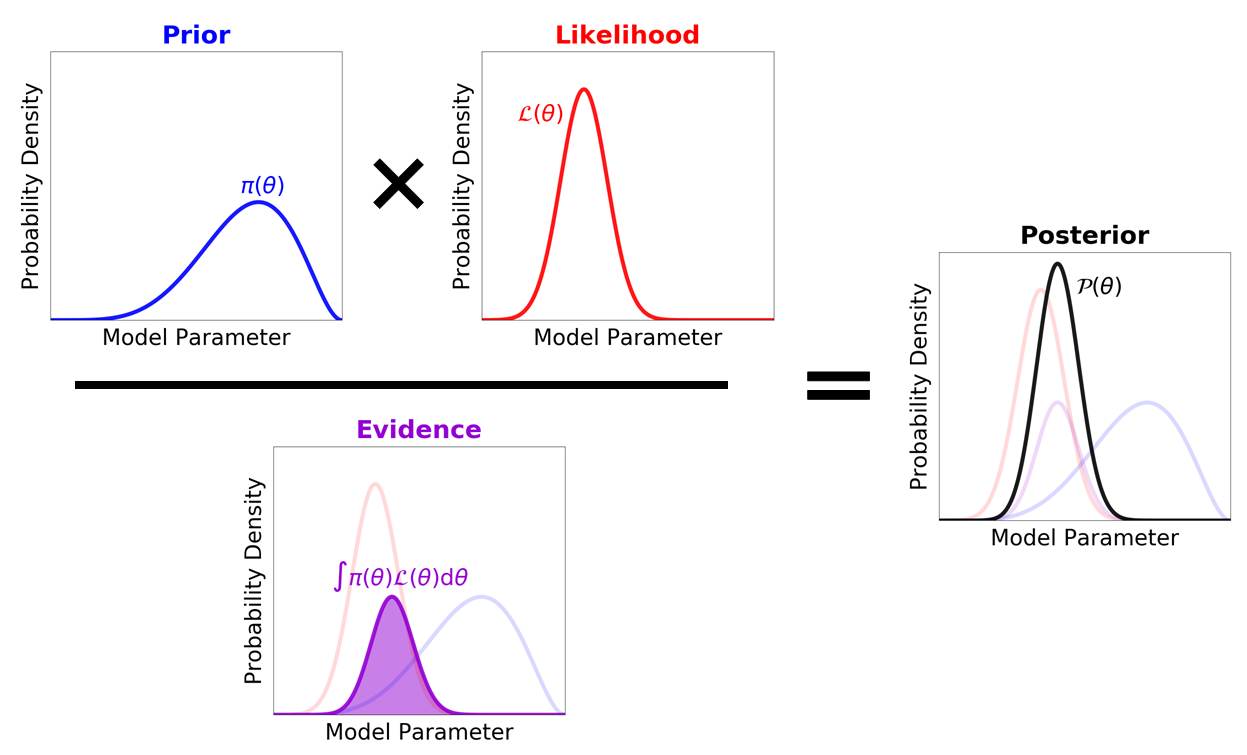
\includegraphics[width=\textwidth]{figures/fig1.png}
\end{center}
\caption{Иллюстрация теоремы Байеса. Постериорная вероятность $\posterior(\params)$ (черный) параметров нашей модели $\params$ основана на комбинации наших предварительных убеждений $\prior(\params)$ (синий) и вероятности $\likelihood(\params)$ (красный), нормированной на общее доказательство $\evidence = \int \prior(\params) \likelihood(\params) \deriv \params$ (фиолетовый) для нашей конкретной модели. Дополнительные подробности см. в \S\ref{sec:bayes}.}\label{fig:bayes}
\end{figure}

Во всей остальной части статьи я буду писать эти четыре термина (вероятность, предшествующее (приор), доказательство, последующее (апостериор)), используя сокращенные обозначения, такие как
\begin{equation}
    \posterior(\params) 
    \equiv \frac{\likelihood(\params)\prior(\params)}{
    \int \likelihood(\params)\prior(\params) \deriv \params}
    \equiv \frac{\likelihood(\params)\prior(\params)}{\evidence}
\end{equation}
где $\posterior(\params) \equiv P(\params_M | \data, M)$ - апостериор, $\likelihood(\params) \equiv P(\data | \params_M, M)$ - вероятность, $\prior(\params) \equiv P(\params_M | M)$ - приоритет, и константа $\evidence \equiv P(\data | M)$ - доказательство. Для удобства я опустил обозначения модели $M$ и данных $\data$, поскольку в большинстве случаев данные и модель считаются фиксированными, но при необходимости я буду вводить их снова.

Прежде чем продолжить, я хотел бы подчеркнуть, что интерпретация любого результата хороша лишь настолько, насколько хороши модели и приорные оценки, которые лежат в их основе. Попытки исследовать последствия той или иной модели с помощью, например, некоторых методов, описанных в этой статье, по сути, являются второстепенной задачей по сравнению с построением разумной модели с хорошо мотивированными приматами в первую очередь. Я настоятельно рекомендую читателям помнить об этой идее на протяжении всей оставшейся части этой работы.

\subsection*{Упражнение: Среднее значение шума} \label{exercise:bayes}

\subsubsection*{Настройка}

Рассмотрим случай, когда у нас есть станции мониторинга температуры, расположенные по всему городу. Каждая станция $i$ проводит зашумленное измерение $\hat{T}_i$ температуры в любой день с некоторым шумом измерения $\sigma_i$. Мы будем считать, что наши измерения $\hat{T}_i$ следуют \textbf{нормальному (т.е. гауссовскому) распределению} со средним $T$ и стандартным отклонением $\sigma_i$, таким, что
\begin{equation*}
    \hat{T}_i \sim \Normal{T}{\sigma_i}
\end{equation*}
Это означает, что вероятность
\begin{equation*}
    P(\hat{T}_i|T,\sigma_i) \equiv \Normal{T}{\sigma_i}
    = \frac{1}{\sqrt{2\pi\sigma_i^2}}
    \exp\left[-\frac{1}{2}\frac{(\hat{T}_i - T)^2}{\sigma_i^2}\right]
\end{equation*}
для каждого наблюдения и
\begin{equation*}
    P(\{ \hat{T}_i \}_{i=1}^{n} | T, \{ \sigma_i \}_{i=1}^{n})
    = \prod_{i=1}^{n} P(\hat{T}_i|T,\sigma_i)
\end{equation*}
для набора из $n$ наблюдений.

Предположим, что у нас есть пять независимых шумных измерений температуры (в градусах Цельсия) с нескольких станций мониторинга
\begin{equation*}
    \hat{T}_1 = 26.3, \: \hat{T}_2 = 30.2, \: \hat{T}_3 = 29.4, 
    \hat{T}_4 = 30.1, \: \hat{T}_5 = 29.8
\end{equation*}
с соответствующими неопределенностями
\begin{equation*}
    \sigma_1 = 1.7, \: \sigma_2 = 1.8, \: \sigma_3 = 1.2, 
    \sigma_4 = 0.5, \: \sigma_5 = 1.3
\end{equation*}

Рассматривая исторические данные, мы обнаруживаем, что типичная базовая температура $T$ в течение подобных дней имеет примерно нормальное распределение со средним значением $T_{\rm prior}=25$ и вариацией $\sigma_{\rm prior} = 1,5$:
\begin{equation*}
    T \sim \Normal{T_{\rm prior}=25}{\sigma_{\rm prior}=1.5}
\end{equation*}

\subsubsection*{Постановка проблемы}

Используя эти предположения, вычислите:
\begin{enumerate}
	\item приор $\prior(T)$,
	\item вероятность $\likelihood(T)$, и
	\item апостериор $\posterior(T)$.
\end{enumerate}
учитывая наши наблюдаемые данные $\{ \hat{T}_i \}$ и ошибки $\{ \sigma_i \}$
в диапазоне температур $T$. Как различаются эти три условия?
Похоже ли предварительное предположение на хорошее? Почему или почему нет?

\section{Для чего нужны апостериорные распределения?} \label{sec:what}

Выше я описал, как теорема Байеса способна объединить наши предварительные убеждения и наблюдаемые данные в новую апостериорную оценку $\posterior(\params)\propto \likelihood(\params)\prior(\params)$. Однако это только половина проблемы. Получив апостериор, мы должны затем \textit{использовать} его, чтобы сделать выводы об окружающем нас мире. В целом, способы, которыми мы хотим использовать апостериоры, делятся на несколько широких категорий:
\begin{enumerate}
\item \textbf{Сделать обоснованные предположения}:
сделать обоснованное предположение о том, какие параметры лежат в основе модели.
\item \textbf{Квантование неопределенности}:
определить ограничения на диапазон возможных значений параметров модели.
\item \textbf{Генерирование прогнозов}: предельная оценка неопределенности параметров модели для предсказания наблюдаемых или других переменных, зависящих от параметров модели.
\item \textbf{Сравнение моделей}:
использование доказательств, полученных с помощью различных моделей, для определения того, какая модель более благоприятна.
\end{enumerate}

Для достижения этих целей нам часто интереснее попытаться использовать апостериор для оценки различных ограничений на сами параметры $\params$ или другие величины $f(\params)$, которые могут быть основаны на них. Это часто зависит от маргинализации неопределенностей, характеризуемых нашим апостериором (через правдоподобие и приоритет). Доказательство $\evidence$, например, снова является просто интегралом правдоподобия и предшествования по всем возможным параметрам:
\begin{equation}
    \evidence 
    = \int \likelihood(\params) \prior(\params) \deriv \params
    \equiv \int \tilde{\posterior}(\params) \deriv \params
\end{equation}
где $\tilde{\posterior}(\params) \equiv \likelihood(\params) \prior(\params)$
это ненормированный апостериор.

Аналогично, если мы изучаем поведение подмножества "интересных'' параметров $\params_{\rm int}$ из $\params = \{ \params_{\rm int}, \params_{\rm nuis} \}$, мы хотим маргинализировать поведение оставшихся "неприятных'' параметров $\params_{\rm nuis}$, чтобы увидеть, как они могут повлиять на $\params_{\rm int}$. Этот процесс довольно прост, если известно все апостериорное значение $\params$:
\begin{equation}
    \posterior(\params_{\rm int})
    = \int \posterior(\params_{\rm int}, \params_{\rm nuis}) \, \deriv \params_{\rm nuis}
    = \int \posterior(\params) \deriv \params_{\rm nuis}
\end{equation}

Другие величины, как правило, могут быть получены из \textbf{значения ожидания} различных функций $f(\params)$, зависящих от параметров, по отношению к апостериору:
\begin{equation}
    \meanwrt{f(\params)}{\posterior} 
    \equiv \frac{\int f(\params) \posterior(\params) \deriv \params}
    {\int \posterior(\params) \deriv \params} 
    = \frac{\int f(\params) \tilde{\posterior}(\params) \deriv \params}
    {\int \tilde{\posterior}(\params) \deriv \params} 
    = \int f(\params) \posterior(\params) \deriv \params
\end{equation}
поскольку $\int \posterior(\params) \deriv \params = 1$ по определению и $\tilde{\posterior}(\params) \propto \posterior(\params)$. Это представляет собой средневзвешенное значение $f(\params)$, где при каждом значении $\params$ мы взвешиваем полученное значение $f(\params)$, исходя из вероятности того, что это значение является правильным.

В совокупности мы видим, что почти во всех случаях нам интереснее вычислять интегралы по апостериору, чем знать сам апостериор. Другими словами, апостериор редко бывает полезен сам по себе; в основном он становится полезным при интегрировании по нему.
% Some schematic illustrations of this process are shown in \autoref{fig:expectations}.

% \begin{figure}
% \begin{center}
% 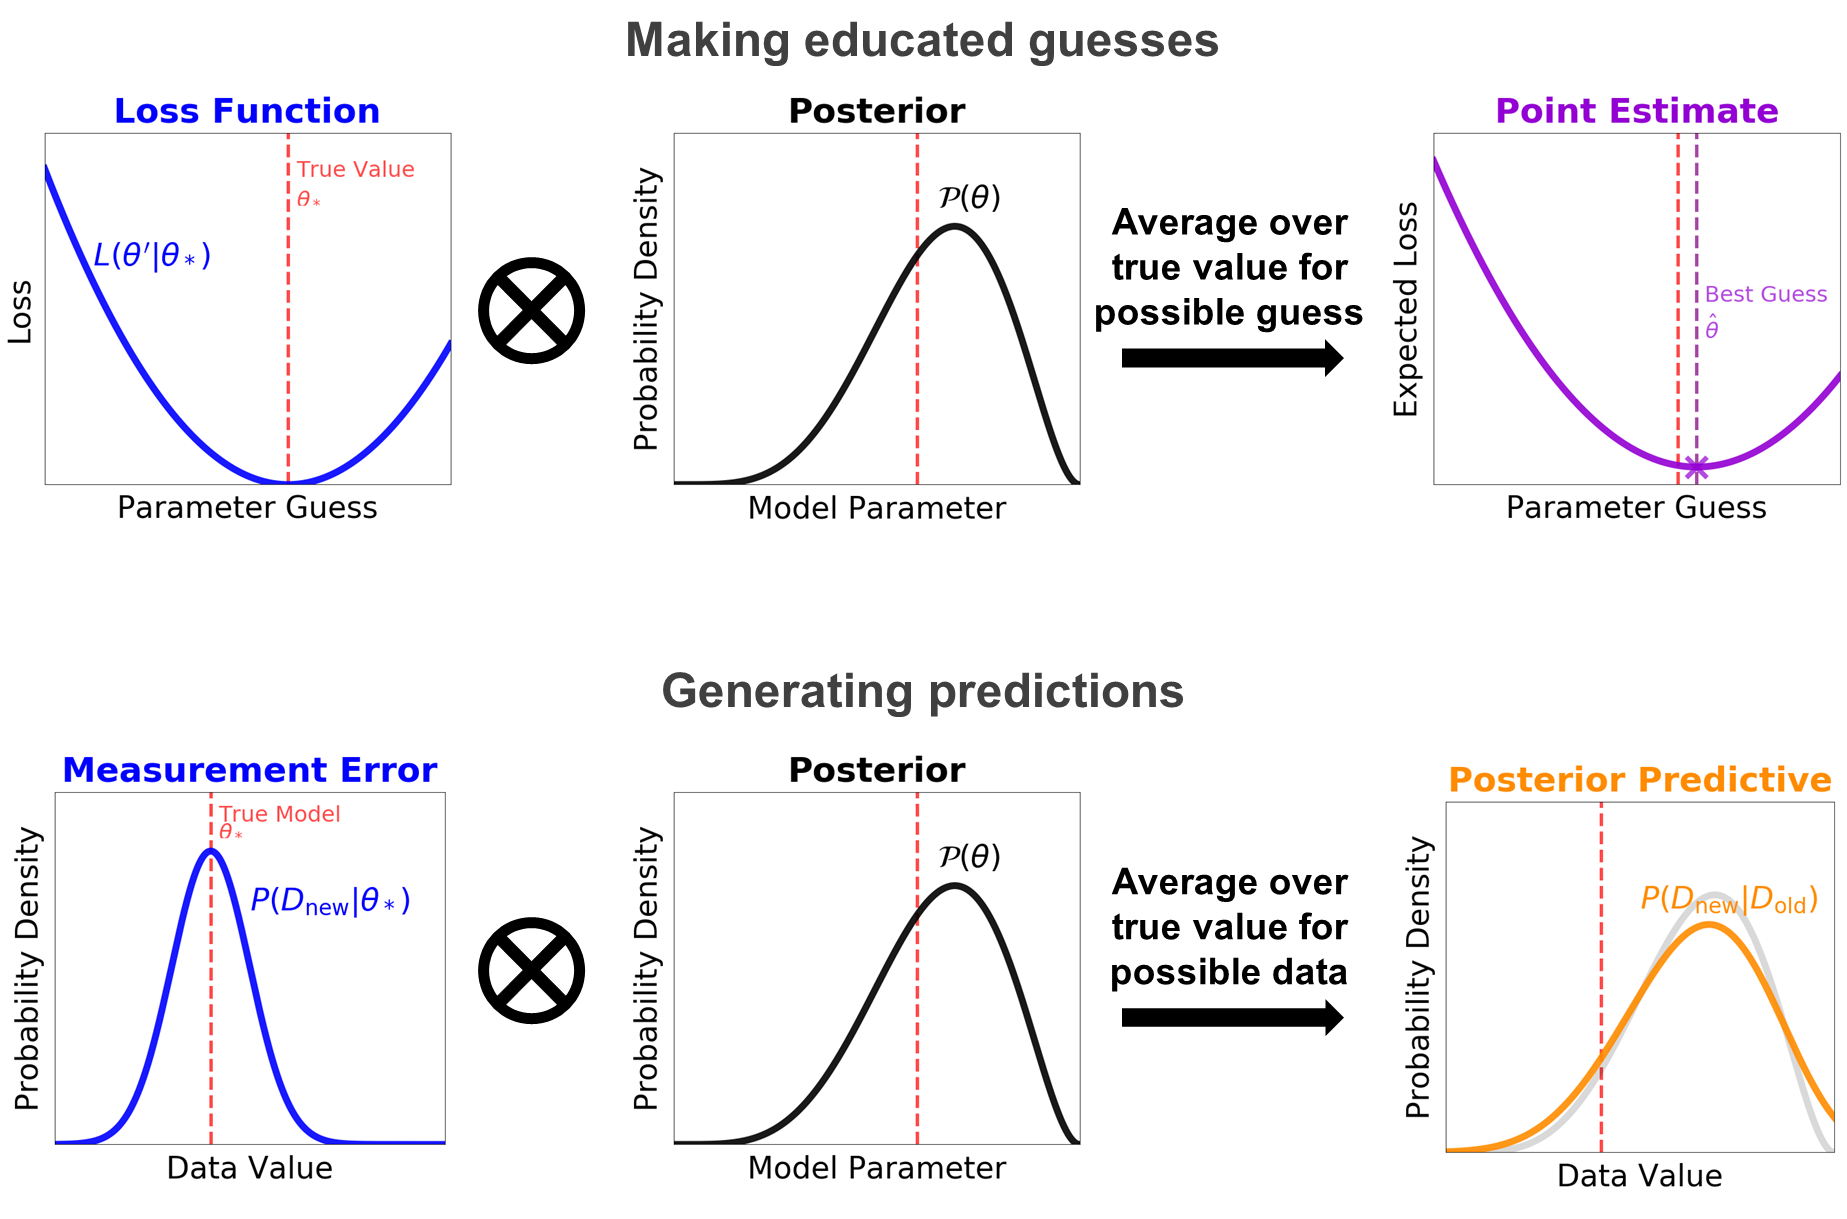
\includegraphics[width=\textwidth]{figures/fig2.png}
% \end{center}
% \caption{Two schematic examples of how using Bayes' Theorem in practice often
% means computing expectation values (i.e. integrating over) 
% the posterior $\posterior(\params)$.
% In the top panel, we illustrate how to use $\posterior(\params)$ to derive
% an optimal point estimate $\hat{\params}$. We want to choose the point estimate
% that minimizes the loss $L(\hat{\params}|\params_*)$ (blue) for with respect to
% the true underlying value $\params_*$ (red). Since we only know
% $\posterior(\params)$ (black), however, we have to average over all possible values
% of $\params_*=\params$ to find an estimate that performs optimally across all
% possibilities (purple). In the bottom panel, we are interested instead in predicting
% some value $\data_{\rm new}$ that future measurements may take. If the true
% $\params_*$ (red) was known, computing 
% $P(\data_{\rm new}|\params_*)$ would be straightforward.
% However, since we only know $\posterior(\params)$ (black) we instead must average
% over all possible values of $\params_*=\params$ when making our prediction
% for $P(\data_{\rm new}|\data_{\rm old})$ (orange).
% See \S\ref{sec:what} for additional details.
% }\label{fig:expectations}
% \end{figure}

Это различие между оценкой ожиданий и других интегралов по апостериору и оценкой апостериора как такового является ключевым элементом байесовского вывода. Это различие имеет огромное значение, когда дело доходит до практического выполнения выводов, поскольку часто бывает так, что мы можем получить отличную оценку $\meanwrt{f(\params)}{\posterior}$, даже если у нас крайне плохая оценка $\posterior(\params)$ или $\tilde{\posterior}(\params)$.

Ниже приводится более подробная информация, чтобы проиллюстрировать, как конкретные категории, описанные выше, превращаются в конкретные интегралы по (ненормированному) заднему числу. Пример показан на {\color{red} \autoref{fig:corner}}.

\begin{figure}
\begin{center}
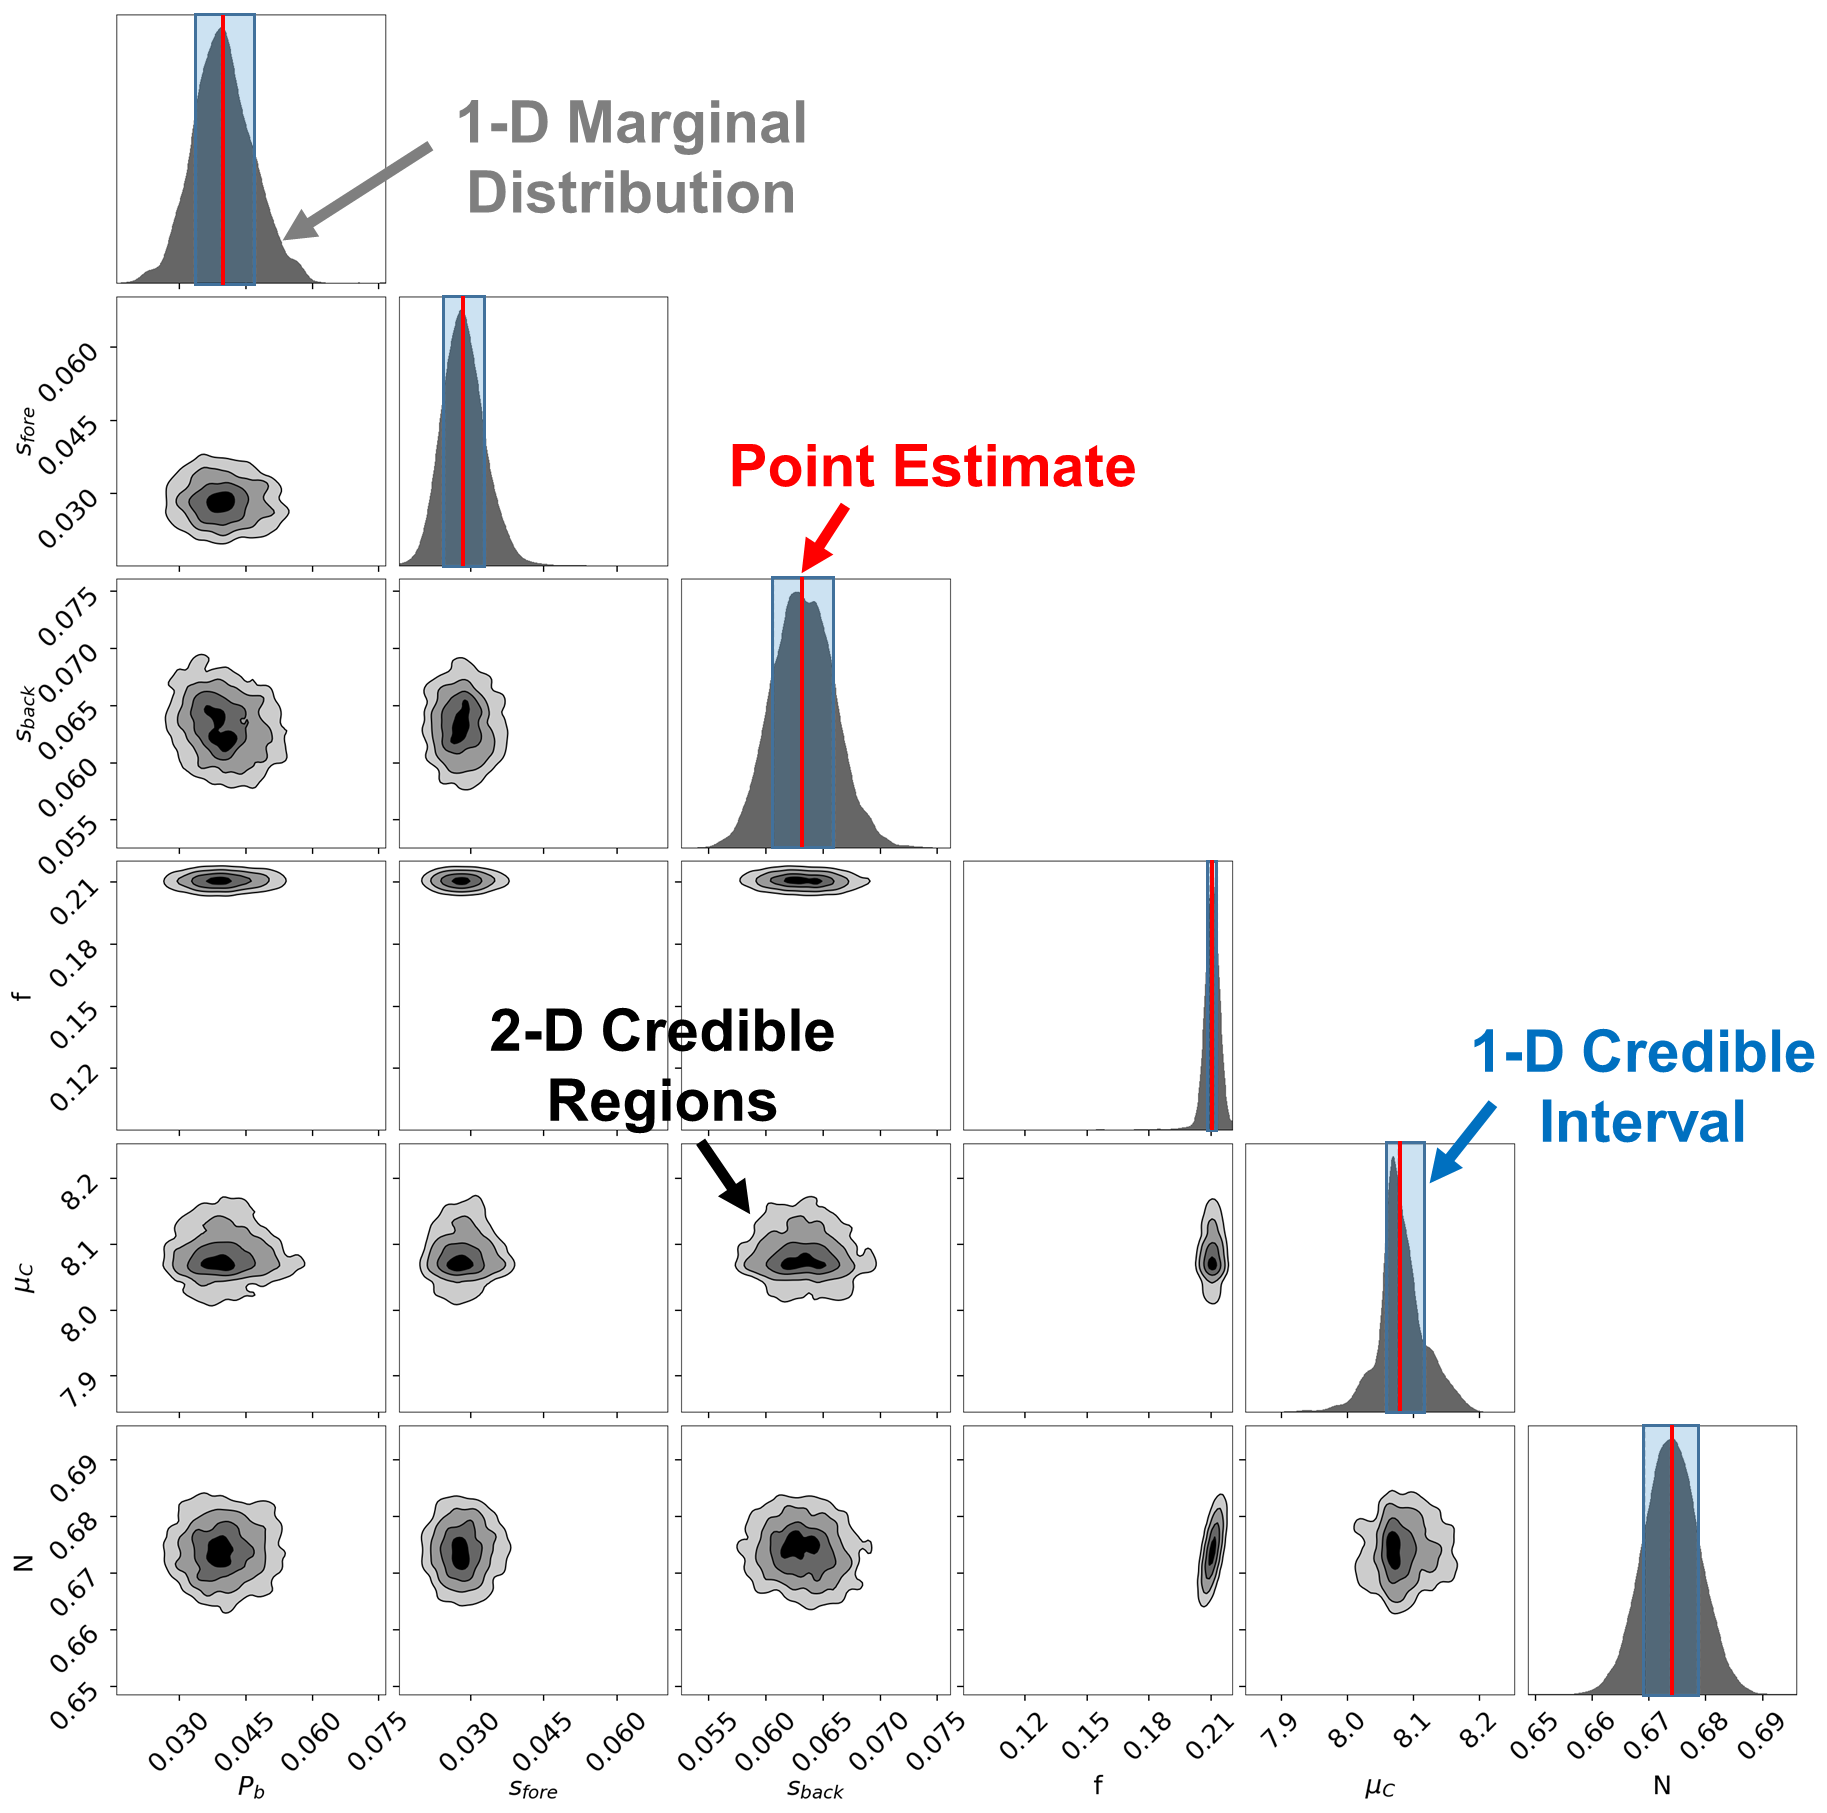
\includegraphics[width=\textwidth]{figures/fig2_v2.png}
\end{center}
\caption{Угловой график, показывающий пример практического использования астериоров. На каждой из верхних панелей показано одномерное маргинальное апостериорное распределение для каждого параметра (серый), а также соответствующие медианные точечные оценки (красный) и 68\%-ные доверительные интервалы (синий). На каждой центральной панели показаны 10\%, 40\%, 65\% и 85\% доверительные области для каждого двумерного маргинального апостериорного распределения. Дополнительные сведения см. в разделе \S\ref{sec:what}.
}\label{fig:corner}
\end{figure}

\subsection{Делаем обоснованные предположения} \label{subsec:guess}

Один из основных постулатов байесовского вывода состоит в том, что мы не знаем ни истинной модели $M_*$, ни ее истинных базовых параметров $\params_*$, характеризующих наблюдаемые данные: имеющаяся у нас модель $M$ почти всегда является упрощением того, что происходит на самом деле. Однако если мы предположим, что наша текущая модель $M$ верна, то мы можем попытаться использовать наш апостериор $\posterior(\params)$, чтобы предложить \textbf{точечную оценку} $\hat{\params}$, которая, по нашему мнению, является довольно хорошим предположением для истинного значения $\params_*$.

Что именно считается ``хорошим''? Это зависит от того, что именно нас волнует. В общем случае, мы можем оценить ``хорошо'', задав противоположный вопрос: насколько сильно мы наказаны, если наша оценка $\hat{\params} \neq \params_*$ окажется неверной? Часто для этого используется \textbf{функция потерь} $L(\hat{\params}|\params_*)$, которая наказывает нас, когда наша точечная оценка $\hat{\params}$ отличается от $\params_*$. Примером общей функции потерь является $L(\hat{\params}|\params_*) = |\hat{\params} - \params_*|^2$ (т.е. квадратичная потеря), где неправильное предположение наказывается квадратом величины расхождения между предположением $\hat{\params}$ и истинным значением $\params_*$.

К сожалению, мы не знаем, каково реальное значение $\params_*$, чтобы оценить истинный проигрыш. Однако мы можем поступить следующим образом и вычислить \textbf{ожидаемый убыток}, усредненный по всем возможным значениям $\params_*$, основываясь на нашем апостериоре:
\begin{equation}
    L_\posterior(\hat{\params})
    \equiv \meanwrt{L(\hat{\params}|\params)}{\posterior}
    = \int L(\hat{\params}|\params) \posterior(\params) \deriv \params
\end{equation}
Тогда разумным выбором для $\hat{\params}$ будет значение, которое минимизирует этот ожидаемый убыток вместо фактического (неизвестного) убытка:
\begin{equation}
    \hat{\params} 
    \equiv \argmin_{\params'} \left[L_\posterior(\params')\right]
\end{equation}
где $\argmin$ указывает на значение (аргумент) $\params'$, которое минимизирует ожидаемый убыток $L_\posterior(\params')$.

Хотя эта стратегия может работать для любой произвольной функции потерь, решение $\hat{\params}$ часто требует использования численных методов и повторного интегрирования по $\posterior(\params)$. Однако для определенных функций потерь существуют аналитические решения. Например, легко показать (и это будет интересным упражнением для заинтересованного читателя), что оптимальная оценка точки $\hat{\params}$ при квадратичных потерях - это просто среднее.

\subsection{Quantifying Uncertainty} \label{subsec: guess}

Во многих случаях нас интересует не просто вычисление предсказания $\hat{\params}$ для $\params_*$, но и ограничение области $\credible(\params)$ возможных значений, внутри которой $\params_*$ может лежать с некоторой долей уверенности. Другими словами, можем ли мы построить область $\credible_X$ такую, что мы считаем, что существует $X\%$ шанс, что она содержит $\params_*$?

Существует множество возможных определений этой \textbf{вероятной области}. Одно из общих определений - это область выше некоторого порога апостериорности $\posterior_X$, в которой содержится $X\%$ апостериорности, т.е. где
\begin{equation}
    \int_{\params \,\in\, \credible_X} \posterior(\params) \deriv \params
    = \frac{X}{100}
\end{equation}
с учетом
\begin{equation}
    \credible_X
    \equiv \left\{ \params : \posterior(\params) \geq \posterior_X \right\}
\end{equation}

Другими словами, мы хотим проинтегрировать наш астериориор по всем $\params$, где значение $\posterior(\params) > \posterior_X$ больше некоторого порога $\posterior_X$, где $\posterior_X$ задается так, чтобы этот интеграл охватывал $X\%$ от полного астериориора. Обычно для $X$ выбирают $68\%$ и $95\%$ (т.е. ``1-сигма`` и ``2-сигма`` доверительные интервалы).

В частном случае, когда наше (маргинальное) апостериори является одномерным, \textbf{достоверные интервалы} часто определяются с помощью \textbf{перцентилей}, а не порогов, где место $x_p$ расположения $p$-го перцентиля определяется как
\begin{equation}
    \int_{-\infty}^{x_p} \posterior(x) \deriv x = \frac{p}{100}
\end{equation}
Мы можем использовать их для определения достоверной области $[x_{\rm low}, x_{\rm high}]$, содержащей $Y\%$ данных, взяв $x_{\rm low} = x_{(1-Y)/2}$ и $x_{\rm high} = x_{(1+Y)/2}$. Хотя это приводит к асимметричным пороговым значениям и не обобщается на более высокие размерности, преимуществом этого метода является то, что он всегда охватывает медианное значение $x_{50}$ и имеет равные хвостовые вероятности (т. е. $(1-Y)/2\%$ апостериорного значения с каждой стороны).

В целом, когда в тексте упоминаются "достоверные интервалы'', следует исходить из определения перцентиля, если явно не указано иное.

\subsection{Предсказание} \label{subsec:pred}

Помимо попыток оценить основные параметры нашей модели, мы также часто хотим сделать предсказания других наблюдений или переменных, которые зависят от параметров нашей модели. Если мы считаем, что знаем истинные базовые параметры модели $\params_*$, то этот процесс прост. Однако, учитывая, что у нас есть доступ только к апостериорному распределению $\posterior(\params)$ по возможным значениям $\params_*$, чтобы предсказать, что произойдет, нам нужно сделать маргинализацию на эту неопределенность.

Мы можем количественно выразить эту интуицию с помощью \textbf{апостериорного прогноза} $P(\tilde{\data}|\data)$, который представляет собой вероятность увидеть новые данные $\tilde{\data}$ на основе имеющихся данных $\data$:
\begin{equation}
    P(\tilde{\data}|\data) 
    \equiv \int P(\tilde{\data}|\params) P(\params|\data) \deriv \params
    \equiv \int \tilde{\likelihood}(\params) \posterior(\params) \deriv \params
    = \meanwrt{\tilde{\likelihood}(\params)}{\posterior}
\end{equation}
Другими словами, для гипотетических данных $\tilde{\data}$ мы хотим вычислить ожидаемое значение вероятности $\tilde{\likelihood}(\params)$ по всем возможным значениям $\params$ на основе текущего апостериорного $\posterior(\params)$.

\subsection{Сравнение моделей} \label{subsec:evid}

Последний момент, представляющий интерес во многих байесовских анализах, - это попытка выяснить, благоприятствуют ли данные какой-либо модели (моделям), которую мы предполагаем в нашем анализе. Наш выбор приора или конкретный способ параметризации данных может привести к существенным различиям в интерпретации результатов.

Мы можем сравнить две модели, вычислив коэффициент \textbf{Bayes factor}:
\begin{equation}
    \bayesfactor^{1}_{2}
    \equiv \frac{P(M_{\rm 1}|\data)}{P(M_{\rm 2}|\data)}
    = \frac{P(\data|M_{\rm 1})P(M_{\rm 1})}{P(\data|M_{\rm 2})P(M_{\rm 2})}
    \equiv \frac{\evidence_{\rm 1}}{\evidence_{\rm 2}} 
    \frac{\prior_{\rm 1}}{\prior_{\rm 2}}
\end{equation}
где $\evidence_M$ - снова доказательства в пользу модели $M$, а $\prior_M$ - наша предварительная вера в то, что $M$ верна по сравнению с конкурирующей моделью. В совокупности, фактор Байеса $\bayesfactor$ говорит нам, насколько конкретная модель предпочтительнее другой, учитывая наблюдаемые данные, предельные значения всех возможных параметров модели $\params_M$ и нашу предыдущую относительную уверенность в модели.

Еще раз отметим, что вычисление $\evidence_M$ требует вычисления интеграла $\int \tilde{\posterior}(\params) \deriv \params$ от ненормированного заднего числа $\tilde{\posterior}(\params)$ по $\params$. В сочетании с другими примерами, описанными в этом разделе, становится ясно, что многие распространенные случаи использования байесовского анализа основаны на вычислении интегралов по (возможно, ненормированному) апостериору.

\subsection*{Упражнение: Пересмотр шумного значения} \label{exercise:practice}

\subsubsection*{Setup}

Вернемся к нашему температурному апостериору $\posterior(T)$ из \S\ref{exercise:bayes}. Мы хотим использовать этот результат для получения интересных оценок и ограничений на возможную базовую температуру $T$.

\subsubsection*{Точечные оценки}

\textbf{mean} можно определить как
точечную оценку $\hat{\params}$, которая минимизирует ожидаемые потери
$L_{\posterior}(\hat{\params})$ при \textbf{квадратичных потерях}:
\begin{equation*}
	L_{\rm mean}(\hat{\params}|\params_*) = |\hat{\params} - \params_*|^2
\end{equation*}
\textbf{median} может быть определена как точечная оценка, которая минимизирует
$L_{\posterior}(\hat{\params})$ при \textbf{абсолютных потерях}:
\begin{equation*}
	L_{\rm med}(\hat{\params}|\params_*) = |\hat{\params} - \params_*|
\end{equation*}
\textbf{mode} можно определить как точечную оценку, которая
минимизирует $L_{\posterior}(\hat{\params})$ при \textbf{`катастрофических'' потерях}:
\begin{equation*}
	L_{\rm mode}(\hat{\params}|\params_*) = -\delta(|\hat{\params}-\params_*|)
\end{equation*}
где $\delta(\cdot)$ - \textbf{дельта-функция Дирака}, определенная так, что
\begin{equation*}
	\int f(x)\delta(x-a)\deriv x = f(a)
\end{equation*}

Учитывая эти выражения для среднего, медианы и моды, оцените соответствующие оценки температурных точек $T_{\rm mean}$, $T_{\rm med}$ и $T_{\rm mode}$ из нашего соответствующего постера. Не стесняйтесь экспериментировать с различными аналитическими и численными методами для выполнения этих расчетов.

Мы можем ожидать, что исторические данные, которые мы использовали для наших приор, могут не так хорошо работать сегодня, если произошли некоторые долгосрочные изменения в средней температуре. Например, мы ожидаем, что средняя температура со временем увеличилась, и поэтому мы, возможно, не захотим штрафовать более жаркие температуры $T \geq T_{\rm prior}$ так же сильно, как более холодные $T < T_{\rm prior}$. Мы можем закодировать эту информацию в асимметричной функции потерь, например
\begin{equation*}
    L(\hat{T}|T_*) = 
    \begin{cases}
    |\hat{T} - T_*|^3 & T < T_{\rm prior} \\
    |\hat{T} - T_*| & T \geq T_{\rm prior}
    \end{cases}
\end{equation*}
Какова оптимальная точечная оценка $T_{\rm asym}$, которая минимизирует ожидаемые потери в этом случае?

\subsubsection*{Достоверные интервалы}

Далее попробуем количественно оценить неопределенность. Учитывая апостериор $\posterior(T)$, вычислите 50\%, 80\% и 95\% доверительных интервалов, используя апостериорные пороги $\posterior_X$. Затем вычислите эти доверительные интервалы с помощью перцентилей. Есть ли различия между доверительными интервалами, вычисленными двумя методами? Почему или почему нет?

\subsubsection*{Апостериорное предсказание}

Чтобы распространить наши неопределенности на следующие наблюдения, вычислим апостериорное предсказание $P(\hat{T}_6|\{ \hat{T}_1, \dots, \hat{T}_5 \})$ по диапазону возможных измерений температуры $\hat{T}_6$ для следующих наблюдений с учетом предыдущих пяти $\{ \hat{T}_1, \dots, \hat{T}_5 \}$, предполагая неопределенность $\sigma_6=0$, $\sigma_6=0. 5$, и $\sigma_6=2$.

\subsubsection*{Сравнение моделей}

Наконец, мы хотим выяснить, является ли наша предварительная оценка хорошим предположением. Используя численные методы, вычислите доказательство $\evidence$ для нашего приоритета по умолчанию со средним $T_{\rm prior} = 25$ и стандартным отклонением $\sigma_{\rm prior} = 1,5$. Затем сравните их с доказательствами, полученными на основе альтернативного приоритета, где мы предполагаем, что температура выросла примерно на пятьСравнение моделей градусов со средним $T_{\rm prior} = 30$, но с соответствующей большей неопределенностью $\sigma_{\rm prior} = 3$. Является ли одна модель особенно предпочтительной по сравнению с другой?

\section{Аппроксимация апостериорных интегралов с помощью сеток} \label{sec:grid}

Теперь я хочу изучить методы оценки апостериорных интегралов. Хотя в некоторых случаях (например, в случае сопряженных приоров) их можно вычислить аналитически, в общем случае это не так. Поэтому для правильной оценки величин, подобных тем, что описаны в \S\ref{sec:what}, необходимо использовать численные методы (освещенные в предыдущих упражнениях).

Для начала я рассмотрю случай, когда наш интеграл по $\params$ является одномерным. В этом случае мы можем аппроксимировать его с помощью стандартных численных методов, таких как \textbf{сумма Римана} по \textbf{дискретной сетке} точек:
\begin{equation}
    \meanwrt{f(\params)}{\posterior} 
    = \int f(\params) \posterior(\params) \deriv \params
    \approx \sum_{i=1}^{n} f(\params_i) 
    \posterior(\params_i) \Delta \params_i
\end{equation}
где
\begin{equation}
    \Delta \params_i = \params_{j+1} - \params_{j}
\end{equation}
это просто расстояние между множеством точек $j=1,\dots,n+1$ на базовой сетке и
\begin{equation}
    \params_i = \frac{\params_{j+1} + \params_{j}}{2}
\end{equation}
определяется как средняя точка междуэто просто расстояние между множеством точек $j=1,\dots,n+1$ на базовой сетке иen $\params_j$ и $\params_{j+1}$. \footnote{Выбор $\params_i$ в качестве одной из конечных точек дает последовательное поведение (см. \S\ref{subsec:consistent}) при увеличении числа точек сетки $n \rightarrow \infty$, но обычно приводит к большим погрешностям при конечном $n$.} Как показано на {\color{red} \autoref{fig:riemann}}, этот подход сродни попытке аппроксимировать интеграл с помощью дискретного набора $n$ прямоугольников с высотой $f(\params_i) \posterior(\params_i)$ и шириной $\Delta \params_i$.

\begin{figure}
\begin{center}
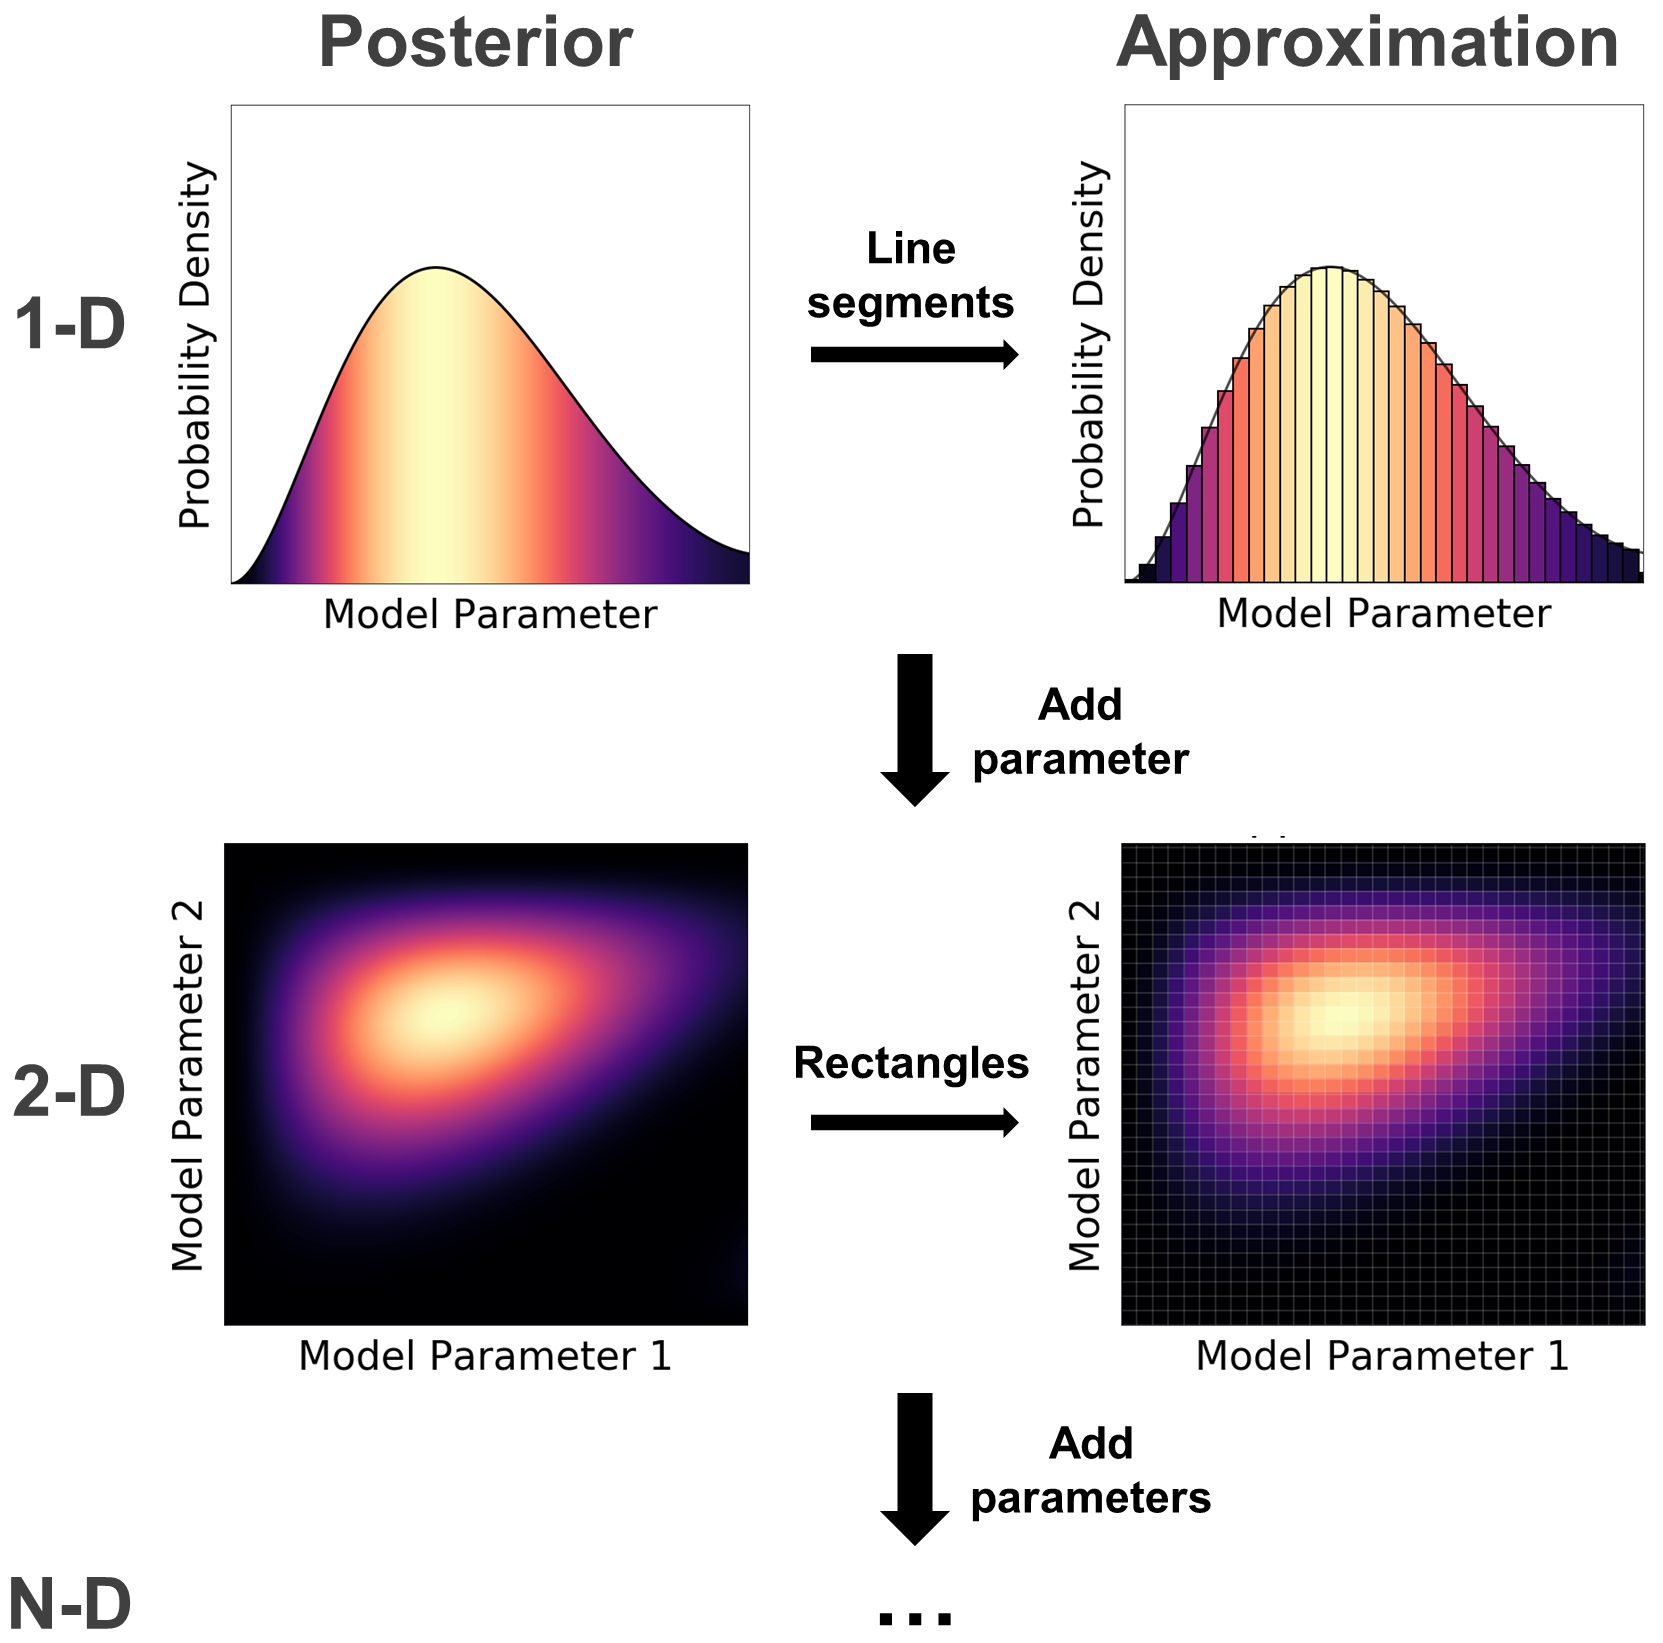
\includegraphics[width=\textwidth]{figures/fig3.png}
\end{center}
\caption{Иллюстрация того, как аппроксимировать апостериорные интегралы с помощью дискретной сетки точек. Мы разбиваем апостериор на смежные области, определяемые позицией $\params_i$ (например, конечной или средней точкой) с соответствующей плотностью $\posterior(\params_i)$ и объемом $\Delta \params_i$ по сетке с $i=1,\dots,n$ элементами. Наш интеграл может быть аппроксимирован сложением каждой из этих областей пропорционально задней массе $\posterior(\params_i) \times \Delta \params_i$, содержащейся в ней. В одномерном пространстве (вверху) эти элементы объема $\Delta\params_i$ соответствуют отрезкам прямых, а в двухмерном (в середине) - прямоугольникам. Это можно обобщить на более высокие измерения (внизу), где мы вместо этого использовали N-D кубоиды. Дополнительные подробности см. в разделе \S\ref{sec:grid}.
}\label{fig:riemann}
\end{figure}

Эту идею можно обобщить на более высокие измерения. В этом случае вместо разбиения интеграла на $n$ одномерных сегментов мы можем разложить его на множество $n$ N-D кубоидов. Тогда вклад каждого из этих кубоидов пропорционален произведению "высоты" $f(\params_i)\posterior(\params_i)$ и \textit{объема}
\begin{equation}
    \Delta \params_i = \prod_{j=1}^{d} \Delta \Theta_{i,j}
\end{equation}
где $\Delta \Theta_{i,j}$ - ширина $i$-го кубоида в $j$-м измерении. См. {\color{red} \autoref{fig:riemann}} для наглядного представления этой процедуры.

Подставив $\posterior(\params) = \tilde{\posterior}(\params)/\evidence$ в значение ожидания и заменив все интегралы их приближениями на основе сетки, получим:
\begin{equation} \label{eqn:exp_grid}
    \meanwrt{f(\params)}{\posterior}
    = \frac{\int f(\params) {\posterior}(\params) \deriv \params}
    {\int {\posterior}(\params) \deriv \params}
    = \frac{\int f(\params) \tilde{\posterior}(\params) \deriv \params}
    {\int \tilde{\posterior}(\params) \deriv \params}
    \approx \frac{\sum_{i=1}^{n} f(\params_i) 
    \tilde{\posterior}(\params_i) \Delta \params_i}
    {\sum_{i=1}^{n}\tilde{\posterior}(\params_i) \Delta \params_i}
\end{equation}
Обратите внимание, что знаменатель теперь представляет собой оценку доказательств:
\begin{equation}
    \evidence 
    = \int \tilde{\posterior}(\params) \deriv \params
    \approx \sum_{i=1}^{n} \tilde{\posterior}(\params_i) \Delta \params_j
\end{equation}
Эта замена ненормированного апостериорного $\tilde{\posterior}(\params)$ на апостериорное $\posterior(\params)$ является важной частью вычисления ожидаемых значений на практике, поскольку мы можем вычислить $\tilde{\posterior}(\params) = \likelihood(\params) \prior(\params)$ непосредственно без знания $\evidence$.

\subsection{Проклятие размерности} \label{subsec:curse}

Хотя этот подход прост, он имеет один непосредственный и серьезный недостаток: общее количество точек сетки увеличивается \textit{экспоненциально} с ростом числа измерений. Например, если предположить, что у нас есть примерно $k \geq 2$ точек сетки в каждом измерении, то общее количество точек $n$ в нашей сетке увеличивается как
\begin{equation}
    n \sim \prod_{j=1}^{d} k = k^d
\end{equation}
Это означает, что даже в абсолютном \textit{лучшем} случае, когда $k=2$, мы имеем масштабирование $2^d$.

Это ужасное масштабирование часто называют \textbf{проклятием размерности}. Эта экспоненциальная зависимость оказывается общим свойством высокоразмерных распределений (т.е. апостериоров моделей с большим числом параметров), к которому я вернусь позже в \S\ref{sec:sampling}.

\subsection{Эффективный размер выборки} \label{subsec:ess}

Помимо экспоненциального масштабирования размерности, у использования сеток есть и более тонкий недостаток. Поскольку мы не знаем форму распределения заранее, вклад каждой части сетки (т.е. каждого N-D кубоида) может быть крайне неравномерным в зависимости от структуры сетки. Другими словами, эффективность этого подхода зависит не только от \textit{количества} точек сетки $n$, но и от \textit{места} их распределения. Если мы плохо определим точки сетки, мы можем получить много точек, расположенных в областях, где $\tilde{\posterior}(\params)$ и/или $f(\params)\tilde{\posterior}(\params)$ относительно малы. Это означает, что в их соответствующих суммах будет доминировать небольшое количество точек с гораздо большими относительными "весами". В идеале мы должны увеличить разрешение сетки в тех областях, где апостериорное значение велико, и уменьшить его в других местах, чтобы смягчить этот эффект. 

Обратите внимание, что мы используем термин "веса" в предыдущем абзаце вполне осознанно. Если вспомнить нашу первоначальную аппроксимацию, то форма уравнения \eqref{eqn:exp_grid} очень похожа на ту, которая может быть использована для вычисления \textbf{взвешенного выборочного среднего} для $f(\params)$. В этом случае, когда у нас есть $n$ наблюдений $\{ f_1, \dots, f_n \}$ с соответствующими весами $\{ w_1, \dots, w_n \}$, взвешенное среднее находится просто:
\begin{equation} \label{eqn:wt_mean}
    \hat{f}_{\rm mean} \equiv \frac{\sum_{i=1}^{n} w_i f_i}
    {\sum_{i=1}^{n} w_i}
\end{equation}
Действительно, если мы определим
\begin{equation}
    f_i \equiv f(\params_i),
    \quad 
    w_i \equiv \tilde{\posterior}(\params_i) \Delta \params_i
\end{equation}
тогда связь между взвешенным выборочным средним в уравнении \eqref{eqn:wt_mean} и матожиданием от нашей сетки в уравнении \eqref{eqn:exp_grid} становится явной:
\begin{equation}
    \meanwrt{f(\params)}{\posterior}
    \approx \frac{\sum_{i=1}^{n} f(\params_i) 
    \tilde{\posterior}(\params_i) \Delta \params_i}
    {\sum_{i=1}^{n} \tilde{\posterior}(\params_i) \Delta \params_i}
    \equiv \frac{\sum_{i=1}^{n} w_i f_i}
    {\sum_{i=1}^{n} w_i}
\end{equation}

Рассматривая нашу сетку как набор образцов $n$, мы также можем рассмотреть соответствующий \textbf{эффективный размер выборки (ESS)} $n_{\rm eff} \leq n$. В ESS заложена идея о том, что не все наши выборки несут одинаковое количество информации: если у нас есть $n$ образцов, которые очень похожи друг на друга, мы ожидаем получить значительно худшую оценку, чем если у нас есть $n$ образцов, которые сильно отличаются друг от друга. Это происходит потому, что информация в коррелированных выборках, по крайней мере, частично избыточна по отношению друг к другу, причем количество избыточности увеличивается с ростом силы корреляции: в то время как две независимые выборки предоставляют совершенно уникальную информацию о распределении и никакой информации друг о друге, две коррелированные выборки вместо этого предоставляют некоторую информацию друг о друге за счет основного распределения.

\begin{figure}
\begin{center}
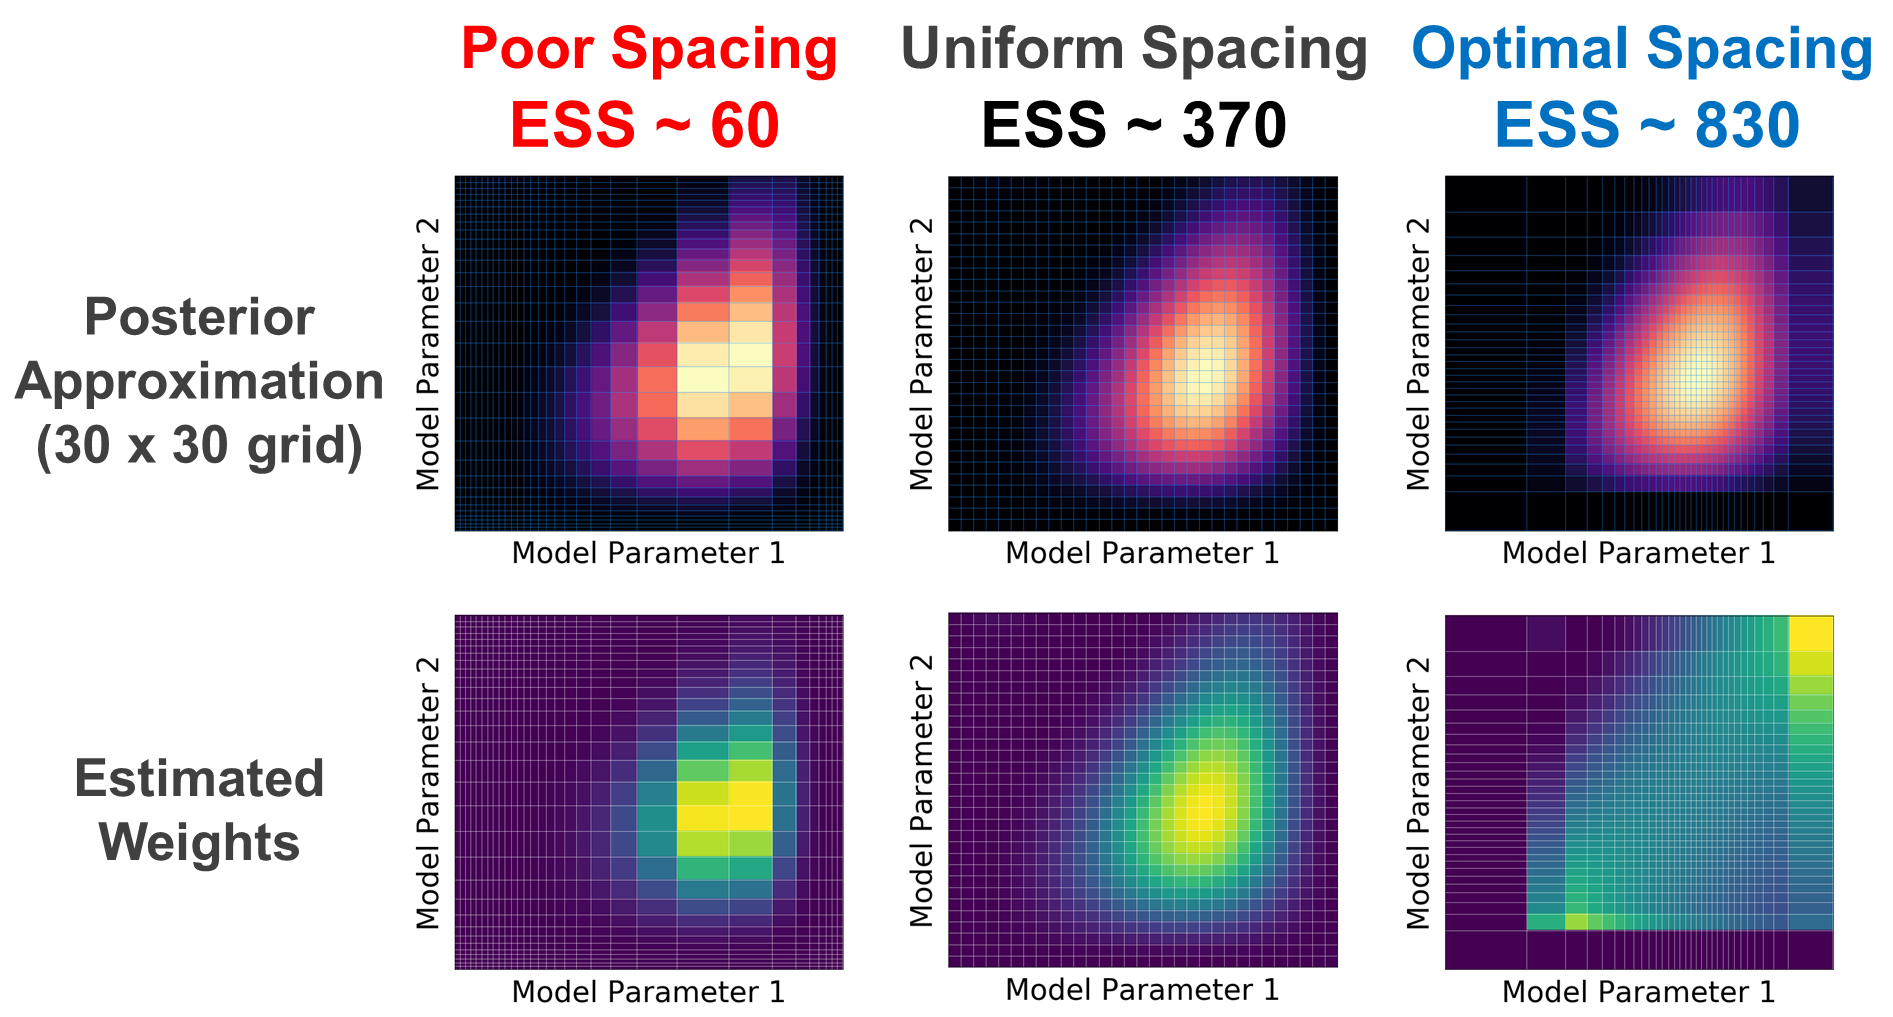
\includegraphics[width=\textwidth]{figures/fig4.png}
\end{center}
\caption{Пример того, как изменение расстояния (элементов объема) сетки может кардинально повлиять на связанную с ней оценку апостериальных интегралов. На игрушечном двухмерном апостериорном интеграле $\posterior(\params)$ простое изменение расстояния между элементами соответствующей двухмерной сетки $30 \times 30$ резко влияет на эффективный размер выборки (ESS) (см. \S\ref{subsec:ess}). Различия между плохим расстоянием (слева), равномерным расстоянием (в середине) и оптимальным расстоянием (справа) приводят к разнице в ESS на порядок величины, что видно по распределению весов (внизу), связанных с элементами объема каждой сетки. Дополнительные подробности см. в \S\ref{subsec:ess}.
}\label{fig:ess}
\end{figure}

Возвращаясь к сеткам, это соответствие означает, что теоретически мы можем получить оценку матожидания $\meanwrt{f(\params)}{\posterior}$, которая будет \textit{по крайней мере} столь же хороша, как и та, которую мы могли бы иметь в настоящее время, используя меньшее число $n_{\rm eff} \leq n$ точек сетки, если бы мы могли распределить их более эффективно. Это различие имеет значение, потому что ошибки в нашей оценке матожидания обычно масштабируются как функция $n_{\rm eff}$, а не $n$. Например, ошибка среднего значения обычно составляет $\propto n_{\rm eff}^{-1/2}$, а не $\propto n^{-1/2}$.
	
Мы можем количественно оценить идеи, лежащие в основе ESS, как обсуждалось выше, введя формальное определение, следуя \citet{kish65}:
\begin{equation}
    n_{\rm eff} 
    \equiv \frac{\left(\sum_{i=1}^{n} w_i\right)^2}{\sum_{i=1}^{n} w_i^2}
\end{equation}
В соответствии с нашей интуицией, наилучшим случаем при таком определении является тот, в котором все веса равны ($w_i = w$):
\begin{equation}
    n_{\rm eff}^{\rm best}
    = \frac{\left(\sum_{i=1}^{n} w_i\right)^2}{\sum_{i=1}^{n} w_i^2}
    = \frac{(nw)^2}{\sum_{i=1}^{n} w^2}
    = \frac{n^2w^2}{nw^2} = n
\end{equation}
Аналогичным образом, наихудшим случаем является тот, когда весь вес сосредоточен вокруг одной выборки
($w_i = w$ для $i=j$ и $w_i=0$ в противном случае):
\begin{equation}
    n_{\rm eff}^{\rm worst}
    = \frac{\left(\sum_{i=1}^{n} w_i\right)^2}{\sum_{i=1}^{n} w_i^2}
    = \frac{(w)^2}{w^2}
    = 1
\end{equation}
В первом случае (при $n_{\rm eff}^{\rm best}$) каждый из элементов нашей сетки вносит примерно одинаковый вклад в интеграл, а во втором (при $n_{\rm eff}^{\rm worst}$) весь интеграл по существу содержится только в одной из областей N-D кубоида $n$. Иллюстрация такого поведения показана на {\color{red} \autoref{fig:ess}}.

\subsection{Сходимость и согласованность} \label{subsec:consistent}

Теперь, когда я обрисовал взаимосвязь между структурой нашей сетки и ESS, я хочу рассмотреть два последних вопроса: \textbf{сходимость} и \textbf{согласованность}. Сходимость - это идея о том, что, хотя наши оценки по $n$ выборкам (точкам сетки) могут быть шумными, они приближаются к некоторому надежному значению по мере того, как $n \rightarrow \infty$:
\begin{equation}
    \lim_{n \rightarrow \infty} \frac{\sum_{i=1}^{n} f(\params_i) 
    \tilde{\posterior}(\params_i) \Delta \params_i}
    {\sum_{i=1}^{n}\tilde{\posterior}(\params_i) \Delta \params_i}
    = C
\end{equation}
Последовательность - это впоследствии идея о том, что значение, к которому мы сходимся, является истинным значением, которое мы хотим оценить:
\begin{equation}
    \lim_{n \rightarrow \infty} \frac{\sum_{i=1}^{n} f(\params_i) 
    \tilde{\posterior}(\params_i) \Delta \params_i}
    {\sum_{i=1}^{n}\tilde{\posterior}(\params_i) \Delta \params_i}
    = \meanwrt{f(\params)}{\posterior}
\end{equation}

\begin{figure}
\begin{center}
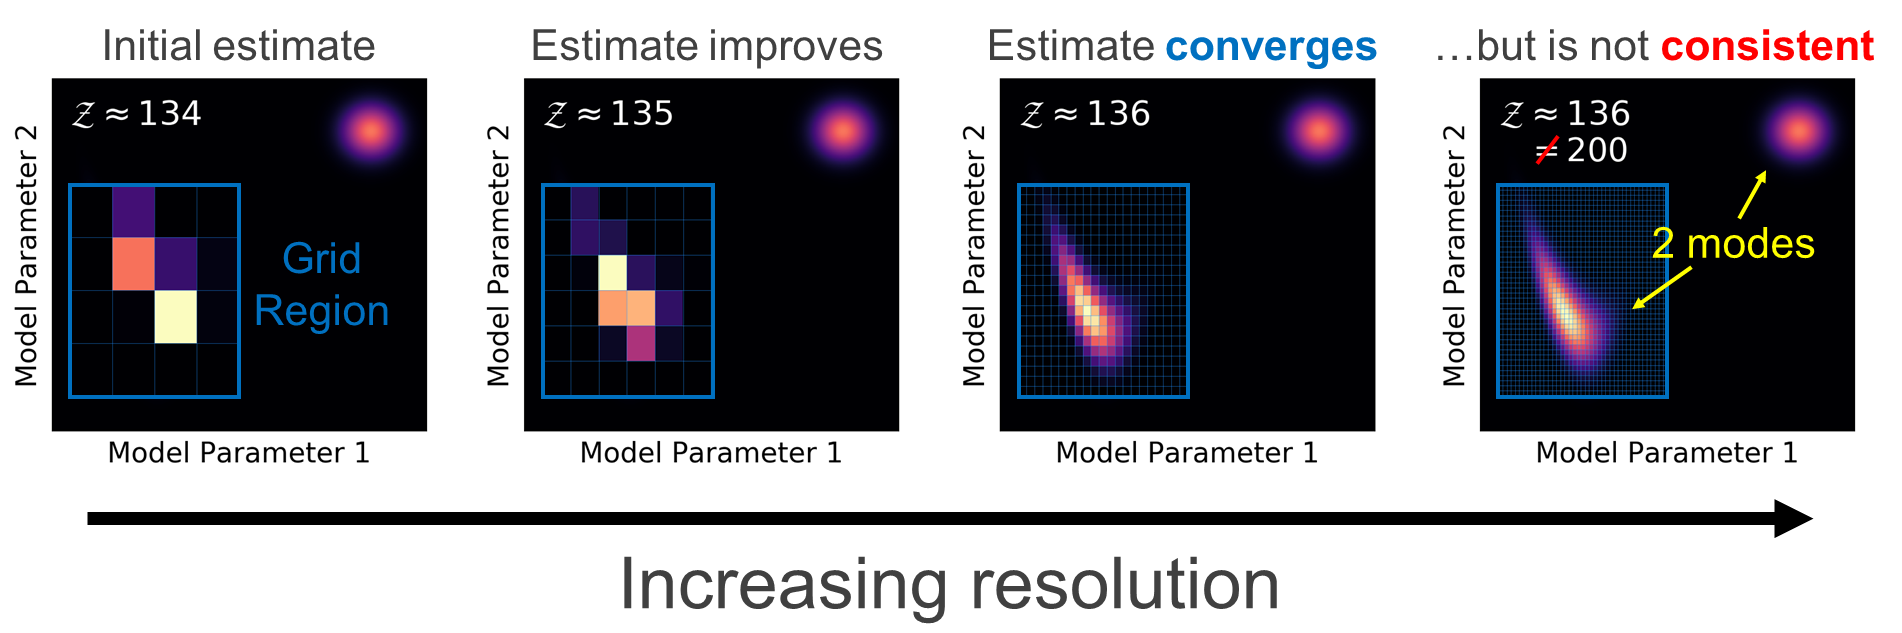
\includegraphics[width=\textwidth]{figures/fig5.png}
\end{center}
\caption{Иллюстрация того, как оценки на основе сетки могут быть \textit{конвергентными} (т.е. сходиться к одному значению по мере увеличения числа точек сетки), но не \textit{консистентными} (т.е. значение, к которому они сходятся, не является правильным ответом). У нашего игрушечного двухмерного ненормированного апостериорного $\tilde{\posterior}(\params)$ есть два режима, которые хорошо разделены с общим доказательством $\evidence = 200$. Если мы не знаем о втором режиме, мы можем определить область сетки, которая охватывает только подмножество всего пространства параметров (слева). Хотя увеличение разрешения сетки в этой области позволяет оценкам $\evidence$ сходиться к единому ответу (слева направо), это не равно правильному ответу $\evidence = 200$, потому что мы пренебрегли вкладом другой компоненты (справа). Дополнительные подробности см. в \S\ref{subsec:consistent}
}\label{fig:conv}
\end{figure}

Легко показать, что \textit{если} матожидание хорошо определено (т.е. существует)\textit{и} сетка покрывает всю область $\params$ (т.е. охватывает наименьшие и наибольшие возможные значения в каждом измерении), то использование сетки является \textbf{согласованным} способом оценки матожидания. Это должно иметь интуитивный смысл: при условии, что наша сетка достаточно обширна в $\params$, так что мы не "пропустим" ни одной области пространства параметров, мы должны быть в состоянии оценить $\meanwrt{f(\params)}{\posterior}$ с произвольной точностью, просто увеличивая разрешение в $\Delta \params$.

К сожалению, мы не знаем заранее, в каком диапазоне значений $\params$ должна находиться наша сетка. В то время как параметры могут лежать в диапазоне $(-\infty, +\infty)$, сетки опираются на элементы конечного объема, поэтому мы должны выбрать некоторое конечное подпространство для сетки. Поэтому, хотя сетки могут давать оценки, которые сходятся к некоторому значению в диапазоне, охватываемом точками сетки, всегда есть вероятность, что значительная часть апостериорного значения лежит за пределами этого диапазона. В таких случаях не гарантируется, что сетки будут последовательными оценщиками $\meanwrt{f(\params)}{\posterior}$. Иллюстрация этой проблемы показана на {\color{red} \autoref{fig:conv}}. Этой фундаментальной проблеме не подвержены методы Монте-Карло, о которых я расскажу в \S\ref{sec:montecarlo}.

\subsection*{Упражнение: Сетки над двумерным гауссовым пространством} \label{exercise:grids}

\subsubsection*{Setup}

Рассмотрим ненормированный апостериор, хорошо аппроксимируемый двумерным гауссовым (нормальным) распределением с центром на $(\mu_x,\mu_y)$ со стандартными отклонениями $(\sigma_x, \sigma_y)$:
\begin{equation*}
    \tilde{\posterior}(x,y) 
    = \exp\left\{-\frac{1}{2}\left[\frac{(x-\mu_x)^2}{\sigma_x^2}
    + \frac{(y-\mu_y)^2}{\sigma_y^2}\right]\right\}
\end{equation*}
Предположим, что мы ожидаем найти, что наше апостериорное значение имеет среднее $0$ и стандартное отклонение $1$. Однако в действительности наше апостериорное значение имеет среднее $(\mu_x,\mu_y)=(-0,3,0,8)$ и стандартное отклонение $(\sigma_x^2,\sigma_y^2)=(2,0,5)$, имитируя обычный случай, когда наши предварительные ожидания и апостериорные выводы несколько расходятся.

\subsubsection*{Оценка на основе сетки}

Мы хотим использовать двумерную сетку для оценки различных форм постреляционных интегралов.
Начиная с равномерно расположенной сетки $5 \times 5$ из $[-2, 2]$, вычислите:
\begin{enumerate}
	\item доказательства $\evidence$,
	\item средние $\meanwrt{x}{\posterior}$
	и $\meanwrt{y}{\posterior}$,
	\item 68\% доверительные интервалы (или ближайшее приближение) 
	$[x_{\rm low}, x_{\rm high}]$ и $[y_{\rm low}, y_{\rm high}]$,
	\ элемент и эффективный размер выборки $n_{\rm eff}$.
\end{enumerate}
Насколько точно каждая из этих величин соответствует тем значениям, которые мы могли бы ожидать? Что говорит нам $n_{\rm eff}/n$ о том, насколько эффективно мы распределили точки сетки?

\subsubsection*{Конвергенция}

Повторите упражнение, используя равномерно расположенную сетку из $20 \times 20$ точек и $100 \times 100$ точек. Прокомментируйте любые различия. Насколько повысилась общая точность? Сходятся ли оценки?

\subsubsection*{Консистенция}

Далее расширьте границы сетки до $[-5, 5]$ и выполните то же упражнение, что и выше. Существенно ли изменились ответы? Если да, то что это говорит нам о согласованности наших предыдущих оценок? Регулируйте плотность и границы сетки до тех пор, пока ответы не станут сходящимися и непротиворечивыми. Помните, что мы не знаем точной формы апостериорных оценок заранее. Что из этого следует в отношении общих проблем при применении сеток на практике?

\subsubsection*{Эффективный размер выборки}

Наконец, изучите, существует ли простая схема настройки расположения точек сетки $x$ и $y$ для максимизации эффективного размера выборки на основе определения, изложенного в \S\ref{subsec:ess}. Если да, то можете ли вы объяснить, почему это работает? Если нет, то почему? Насколько адаптивная регулировка расстояния между сетками может улучшить $n_{\rm eff}$ и общую точность наших оценок по сравнению с эквивалентными равномерно распределенными сетками?

\section{От сеток к методам Монте-Карло} \label{sec:montecarlo}

\subsection{Соединение точек сетки и выборок}
\label{subsec:grid_to_samp}

Ранее я описал, как можно связать оценку $\meanwrt{f(\params)}{\posterior}$ с помощью сетки из $n$ точек с эквивалентной оценкой с помощью набора $n$ выборок $\{ f_1, \dots, f_n\}$ и ряда связанных с ними весов $\{ w_1, \dots, w_n \}$. Основной результат состоит в том, что существует тесная связь между структурой апостериорной сетки и сетки с относительной амплитудой весов $w_i \equiv \tilde{\posterior}(\params_i)\Delta\params_i$ для каждой точки $f_i \equiv f(\params_i)$. Регулировка разрешения сетки влияет на эти веса, при этом более равномерное распределение весов приводит к увеличению ESS, что может улучшить нашу оценку.

Тот факт, что уменьшение расстояния между точками (более плотная сетка) также уменьшает веса, имеет смысл: у нас больше точек, расположенных в этой области, поэтому каждая точка должна получить меньший относительный вес при вычислении $\meanwrt{f(\params)}{\posterior}$. Аналогично, если у нас одинаковые расстояния между точками, но меняется относительная форма заднего плана, то вес этой точки при оценке $\meanwrt{f(\params)}{\posterior}$ также должен измениться соответственно.

Теперь я хочу расширить это базовое соотношение. Теоретически, адаптивное увеличение разрешения нашей сетки позволяет нам лучше контролировать элементы объема $\Delta \params_i$, используемые для получения весов. Если мы достаточно хорошо знаем форму нашего постера, то для больших $n$ мы теоретически должны быть в состоянии настроить $\Delta \params_i$ так, чтобы веса $w_i = \tilde{\posterior}(\params_i)\Delta\params_i$ были равномерными с некоторой желаемой точностью. По проверке, это должно произойти, когда
\begin{equation}
    \Delta \params_i \propto \frac{1}{\tilde{\posterior}(\params_i)}
\end{equation}
для всех $i$.

Если довести эти рассуждения до концептуального предела, то с ростом $n \rightarrow \infty$ мы можем представить, что оцениваем апостериор, используя все большее и большее количество точек сетки, расстояние между которыми $\Delta \params$ меняется как функция от $\params$. Используя это, мы можем определить плотность точек $\proposal(\params)$ на основе изменяющегося разрешения $\Delta\params(\params)$ нашей бесконечно тонкой сетки как функцию $\params$: 
\begin{equation} 
	\proposal(\params)\propto \frac{1}{\Delta\params (\params)} 
\end{equation} 
Этот результат говорит о том, что в континуальном пределе, где $n \rightarrow \infty$, \textit{структура нашей сетки с бесконечным разрешением эквивалентна новому непрерывному распределению} $\proposal(\params)$. Иллюстрация этой концепции показана на {\color{red} \autoref{fig:density}}. Используя $\proposal(\params)$, мы можем переписать наше исходное матожидание в виде
\begin{equation}
    \meanwrt{f(\params)}{\posterior} 
    \equiv \frac{\int f(\params) \tilde{\posterior}(\params) \deriv \params}
    {\int \tilde{\posterior}(\params) \deriv \params}
    = \frac{\int f(\params) \frac{\tilde{\posterior}(\params)}{\proposal(\params)}
    \proposal(\params) \deriv \params}
    {\int \frac{\tilde{\posterior}(\params)}{\proposal(\params)}
    \proposal(\params) \deriv \params}
    = \frac{\meanwrt{f(\params) 
    \tilde{\posterior}(\params)/\proposal(\params)}{\proposal}}
    {\meanwrt{\tilde{\posterior}(\params)/\proposal(\params)}{\proposal}}
\end{equation}
По причинам, которые скоро станут понятны, я буду называть $\proposal(\params)$ распределением \textbf{предложений}.

\begin{figure}
\begin{center}
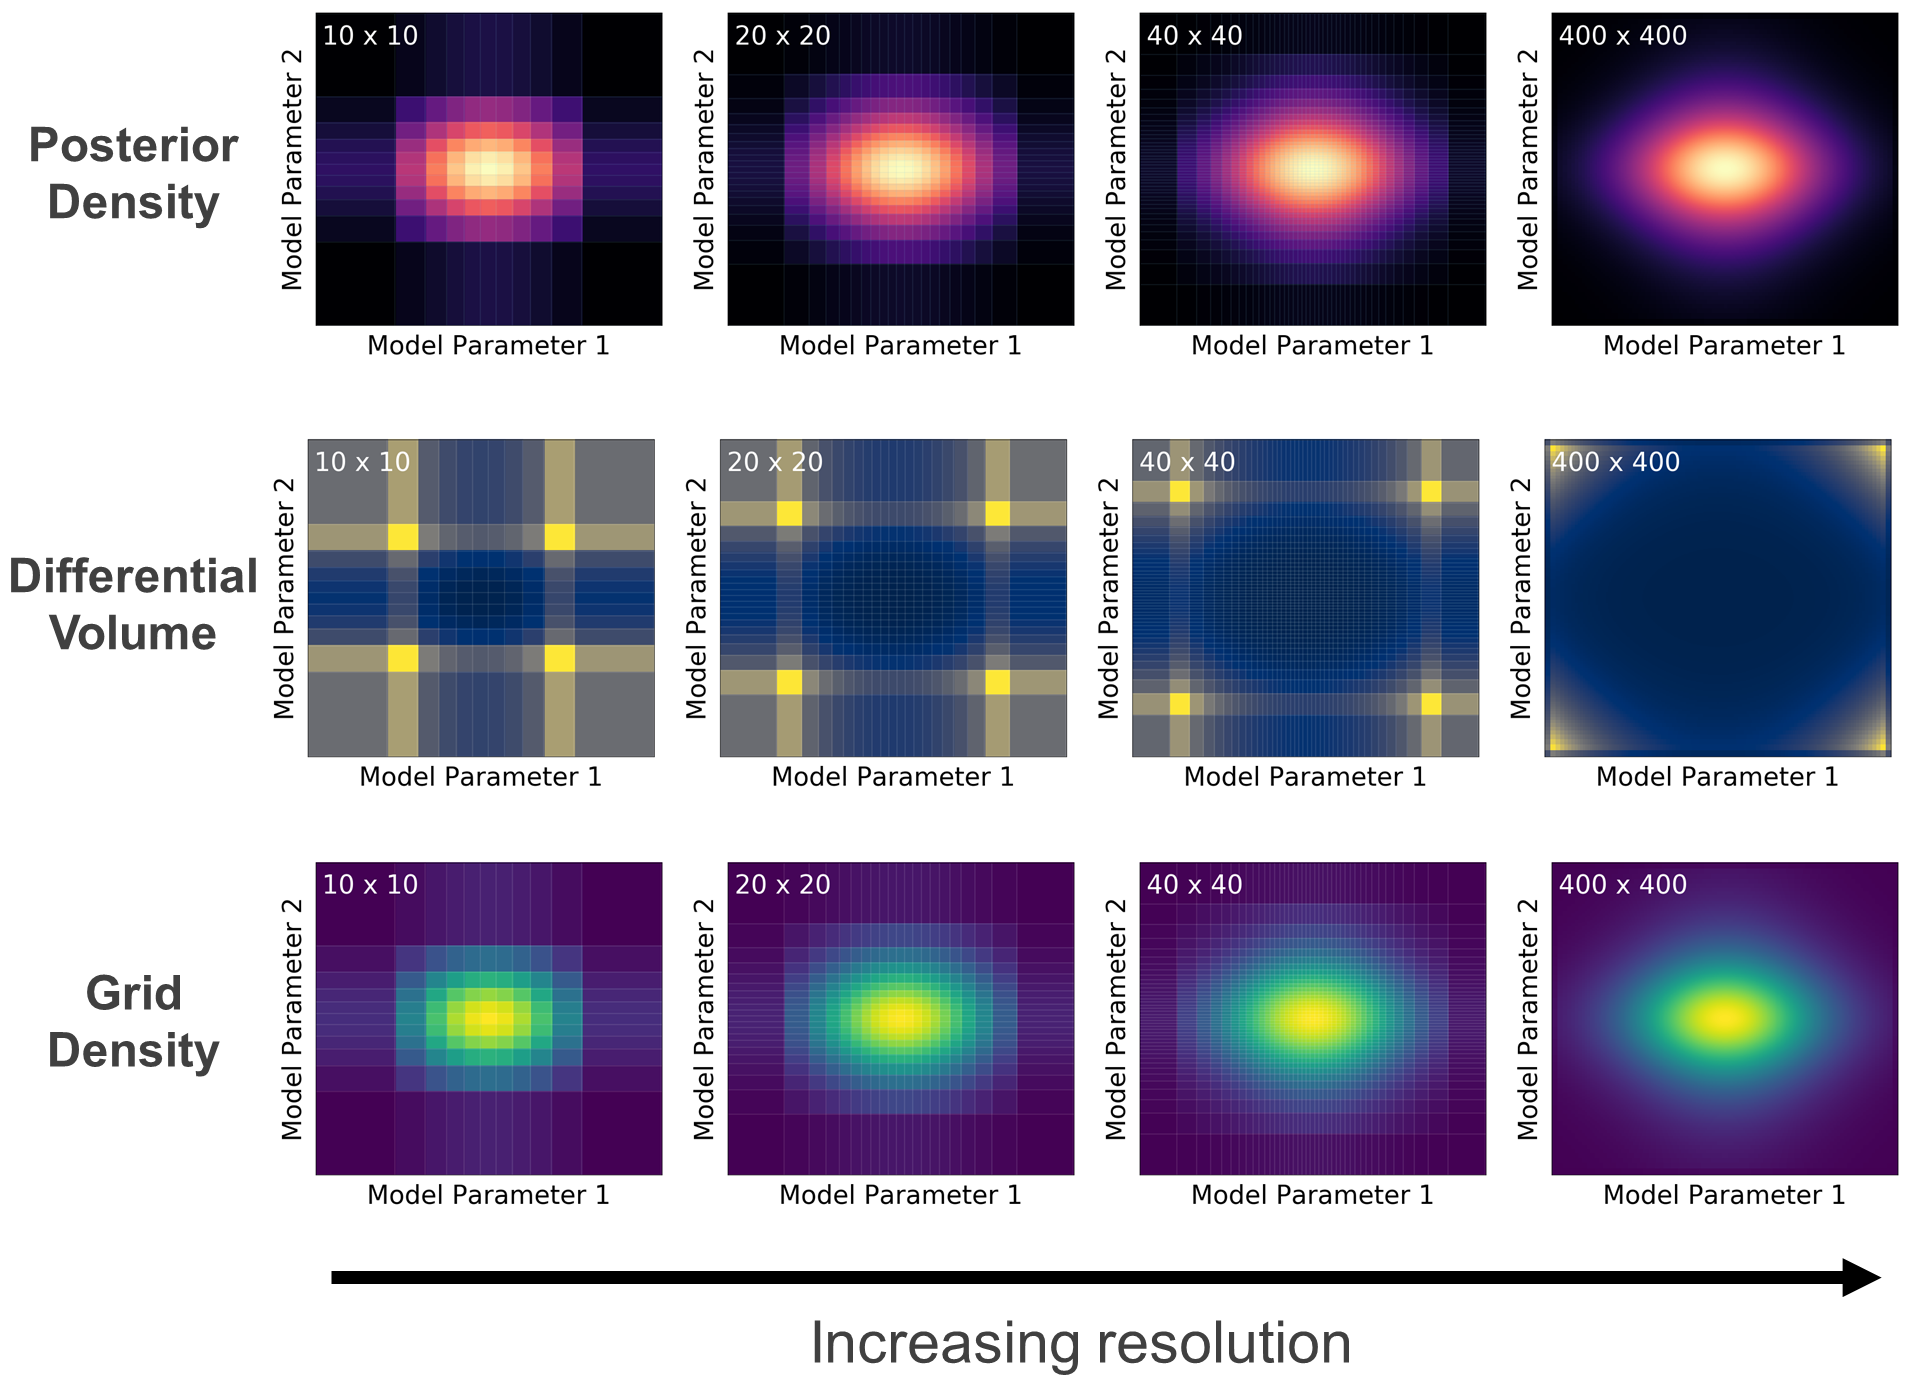
\includegraphics[width=\textwidth]{figures/fig6.png}
\end{center}
\caption{Иллюстрация связи между сетками и непрерывными распределениями плотности. По мере увеличения числа точек сетки наша оценка апостериорного $\posterior(\params)$ улучшается (вверху). Поскольку расстояние между точками сетки меняется, чтобы максимизировать эффективный размер выборки (см. \autoref{fig:ess} и \S\ref{subsec:ess}), элементы дифференциального объема $\Delta \params_i$ меняются в зависимости от нашего местоположения (середина). При дальнейшем увеличении количества элементов объема плотность точек сетки в любом конкретном месте $\rho(\params_i) = [\Delta \params_i]^{-1}$ ведет себя как непрерывная функция $\proposal(\params)$, распределение которой похоже на $\posterior(\params)$ (внизу). Это означает, что мы должны быть в состоянии использовать $\proposal(\params)$ каким-то образом для оценки $\posterior(\params)$. Дополнительные подробности см. в \S\ref{sec:montecarlo}.
}\label{fig:density}
\end{figure}

Сейчас это может показаться математическим трюком: все, что я сделал, это переписал наше исходное \textit{одно} матожидание относительно (ненормированного) апостериорного $\tilde{\posterior}(\params)$ в терминах \textit{два} матожидания относительно распределения предложения $\proposal(\params)$. Эта замена, однако, на самом деле позволяет нам полностью реализовать связь между точками сетки и выборками.

Ранее я показал, что оценка матожидания для точек сетки в точности аналогична оценке, которую мы получили бы, если бы точки сетки были случайными выборками $\{ f_1, \dots, f_n \}$ с соответствующими весами $\{ w_1, \dots, w_n \}$. Однако после того, как мы определили наше ожидание относительно $\proposal(\params)$, это утверждение может стать точным, если мы можем явно генерировать выборки из $\proposal(\params)$.

Давайте быстро рассмотрим, что это значит. Изначально мы рассматривали попытку оценить $\meanwrt{f(\params)}{\posterior}$ по сетке с $n$ точками. Однако в пределе бесконечного разрешения наша сетка становится эквивалентной некоторому распределению $\proposal(\params)$. Используя $\proposal(\params)$, мы можем переписать наше исходное выражение в терминах двух ожиданий, $\meanwrt{f(\params)\tilde{\posterior}(\params)/\proposal(\params)}{\proposal}$ и $\meanwrt{\tilde{\posterior}(\params)/\proposal(\params)}{\proposal}$, над $\proposal(\params)$ вместо $\posterior(\params)$. Это помогает нам, потому что теоретически мы можем оценить эти конечные выражения явно, используя серию из $n$ случайно сгенерированных выборок из $\proposal(\params)$. Из-за случайности, присущей этому подходу, его принято называть \textbf{Монте-Карло} подходом для оценки $\meanwrt{f(\params)}{\posterior}$ из-за исторических связей со случайностью и азартными играми.

На первый взгляд, это удивительное утверждение. Когда мы вычисляем интеграл от функции $f(\params)$ на ограниченной сетке, мы знаем, что в нашем приближении есть некоторая ошибка, связанная с дискретизацией сетки. Эта ошибка полностью \textit{deterministic}: учитывая количество точек сетки $n$ и определенную плотность дискретизации $\proposal(\params)\propto 1/\Delta\params(\params)$, мы каждый раз будем получать один и тот же результат (и ошибку) для $\meanwrt{f(\params)}{\posterior}$.

В отличие от этого, построение $n$ образцов $\{\params_1,\dots,\params_n\}$ из $\proposal(\params)$ является по своей сути рандомным (т.е. стохастическим) процессом, который не похож на сетку точек. И поскольку эти точки по своей природе случайны, фактическое отклонение между нашей оценкой и истинным значением $\meanwrt{f(\params)}{\posterior}$ будет тоже случайным. Таким образом, ``ошибка'' от случайных выборок говорит нам о том, насколько сильно может отличаться наша оценка от многих возможных реализаций нашего случайного процесса при определенном количестве выборок $n$, полученных из $\proposal(\params)$. Тот факт, что мы можем получить примерно эквивалентные оценки на основе этих разных подходов при изменении $n$ и $\proposal(\params)$, лежит в основе связи между точками сетки и выборками.

Есть три основных преимущества перехода от адаптивно распределенной сетки к непрерывному распределению $\proposal(\params)$. Во-первых, сетка всегда будет иметь некоторое минимальное разрешение $\Delta \params_i$, что затрудняет получение приблизительно равномерных весов, ограничивая максимальную ESS на практике. Напротив, теоретически мы можем добиться того, чтобы $\proposal(\params)$ более точно соответствовал апостериору $\posterior(\params)$, что даст большую ESS при фиксированном $n$.

Во-вторых, поскольку мы теперь работаем с \textit{распределениями}, а не с конечным числом точек сетки, мы больше не ограничены некоторым конечным объемом при оценке ожиданий. Поскольку распределения могут лежать в диапазоне $(-\infty, +\infty)$, мы можем гарантировать, что $\proposal(\params)$ обеспечит достаточное \textbf{покрытие} по всем возможным значениям $\params$, по которым может быть определено наше послесловие $\posterior(\params)$. Это означает, что некоторые теоретические вопросы, поднятые в \S\ref{subsec:consistent}, связанные с применением сеток к апостериорам, которые варьируются в диапазоне $(-\infty, +\infty)$, больше не применимы. Таким образом, методы Монте-Карло могут служить \textit{согласованными} оценками для более широкого диапазона возможных апостериорных ожиданий, чем методы на основе сеток, что делает их существенно более гибкими.

Наконец, минимальное число точек сетки всегда экспоненциально растет с размерностью (см. \S\ref{subsec:curse}), независимо от того, сколько параметров нас интересует для маргинализации. Поскольку методы Монте-Карло не полагаются на них, они могут в полной мере использовать преимущества маргинализации по параметрам при оценке ожиданий $\meanwrt{f(\params)}{\posterior}$. Поэтому они менее подвержены этому эффекту (хотя см. \S\ref{subsec:volume}).

\subsection{Выборка по важности} \label{subsec:importance}

% The point about being able to draw samples from
% $\proposal(\params)$ is more than just an option assuming
% the distribution happens to be easy to simulate from.
Как я уже пытался подчеркнуть ранее, основной постулат этой статьи заключается в том, что \textit{мы не знаем, как выглядит $\posterior(\params)$ заранее}. Это означает, что мы не знаем, какая структура сетки даст оптимальную оценку (т.е. максимум ESS) для $\meanwrt{f(\params}{\posterior}$, не говоря уже о том, как она должна вести себя в качестве $\proposal(\params)$ в континуальном пределе. Это дает нам достаточную мотивацию для того, чтобы \textit{выбрать} $\proposal(\params)$ таким образом, чтобы сделать генерацию образцов из него простой и понятной.

Предположив, что мы выбрали такое $\proposal(\params)$, мы можем впоследствии сгенерировать из него серию из $n$ образцов. Предположим, что эти образцы имеют веса $q_i$, связанные с ними, и определим
\begin{equation}
    f(\params_i) \equiv f_i, \quad
    \tilde{\posterior}(\params_i)/\proposal(\params_i) 
    \equiv \tilde{w}(\params_i) \equiv \tilde{w}_i
\end{equation}
наше исходное выражение сводится к
\begin{equation}
    \meanwrt{f(\params)}{\posterior} 
    = \frac{\meanwrt{f(\params) 
    \tilde{w}(\params)}{\proposal}}
    {\meanwrt{\tilde{w}(\params)}{\proposal}}
    \approx \frac{\sum_{i=1}^{n} f_i \tilde{w}_i q_i}
    {\sum_{i=1}^{n} \tilde{w}_i q_i}
\end{equation}
Если далее предположить, что мы выбрали $\proposal(\params)$ так, что можем моделировать выборки, которые \textbf{независимо и идентично распределены (iid)} (т.е. каждая выборка имеет то же распределение вероятности, что и другие, и все выборки взаимно независимы), то соответствующие веса выборок немедленно сводятся к $q_i = 1/n$, и наш результат становится
\begin{equation}
    \meanwrt{f(\params)}{\posterior} 
    \approx \frac{n^{-1} \sum_{i=1}^{n} f_i \tilde{w}_i}
    {n^{-1} \sum_{i=1}^{n} \tilde{w}_i}
\end{equation}
Как и в предыдущем случае с сетками (\S\ref{sec:grid}), знаменатель этого выражения снова является прямым приближением для доказательства
\begin{align}
    \evidence 
    = \int \tilde{\posterior}(\params) \deriv \params
    \approx n^{-1} \sum_{i=1}^{n} \tilde{w}_i
\end{align}

Это дает прямой "рецепт" для оценки нашего исходного значения матожидания:
\begin{enumerate}
	\item Извлеките $n$ iid образцов $\{\params_1, \dots, \params_n \}$.
	из $\proposal(\params)$.
	\item Вычислим их соответствующие веса $\tilde{w}_i =
	\tilde{\posterior}(\params_i)/\proposal(\params_i)$.
	\item Оценить $\meanwrt{f(\params)}{\posterior}$. вычислив $\meanwrt{\tilde{w}(\params)}{\proposal}$ и
	$\meanwrt{f(\params)\tilde{w}(\params)}{\proposal}$ с использованием взвешенных выборочных средних.
\end{enumerate}
Поскольку этот процесс заключается в "перевзвешивании" выборок на основе $\tilde{w}_i$, эти веса часто называют \textbf{весами важности}, а метод - \textbf{Важной выборкой}. Схематическая иллюстрация выборки по важности приведена на {\color{red} \autoref{fig:importance}}.

\begin{figure}
\begin{center}
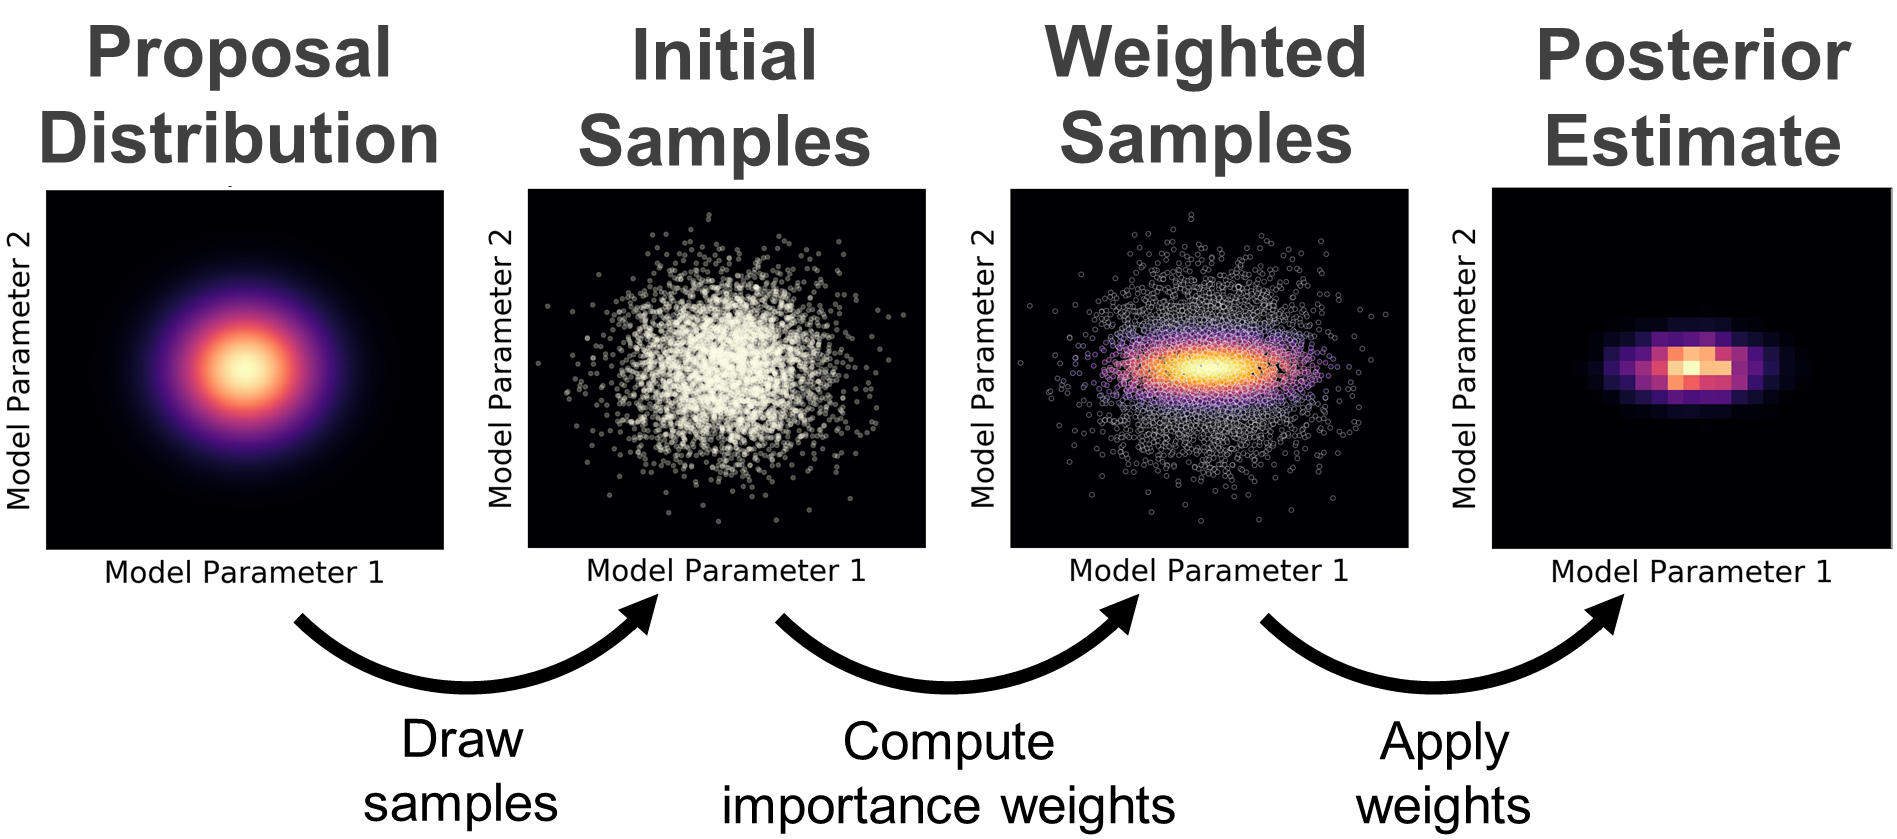
\includegraphics[width=\textwidth]{figures/fig7.png}
\end{center}
\caption{Схематическая иллюстрация Importance Sampling. Сначала мы берем заданное распределение предложений $\proposal(\params)$ (слева) и генерируем из него набор из $n$ иидных выборок (в середине слева). Затем мы взвешиваем каждый образец на основе соответствующей ``важности'' $\tilde{\posterior}(\params)/\proposal(\params)$, которую он имеет в данном месте (середина справа). Затем мы можем использовать эти взвешенные выборки для аппроксимации апостериорных ожиданий (справа). Дополнительные сведения см. в \S\ref{subsec:importance}.
}\label{fig:importance}
\end{figure}

Мы можем интерпретировать веса важности как способ коррекции того, насколько "далека" наша первоначальная догадка $\proposal(\params)$ от истины $\posterior(\params)$. Если в позиции $\params_i$ апостериорная плотность выше по сравнению с плотностью предложения, значит, мы с меньшей вероятностью сгенерировали выборку в этой позиции по сравнению с тем, что было бы, если бы мы брали выборки непосредственно из апостериорной. В результате мы должны увеличить соответствующий вес, чтобы учесть этот ожидаемый дефицит образцов в данной позиции. Если апостериорная плотность меньше плотности предложения, то верна альтернатива, и мы должны уменьшить вес соответствующего образца, чтобы учесть ожидаемый избыток образцов в данной позиции.

\subsection{Примеры стратегий выборки} \label{subsection:samp_strat}

Выборка важности служит полезным первым шагом для понимания того, как веса $\{ \tilde{w}_1, \dots, \tilde{w}_n \}$ для соответствующего набора образцов $n$ связаны с различными стратегиями выборки Монте-Карло.

Например, одним из распространенных подходов является равномерная генерация образцов в пределах некоторого кубоида с объемом $V$. Тогда распределение предложения будет иметь вид
\begin{equation}
    \proposal^{\rm unif}(\params) =
    \begin{cases}
    1/V & \params \: {\rm in\:cuboid} \\
    0 & {\rm otherwise}
    \end{cases}
\end{equation}
Соответствующие веса важности впоследствии будут просто пропорциональны апостериору в данной позиции:
\begin{equation}
    \tilde{w}_i^{\rm unif}
    = \frac{\tilde{\posterior}(\params_i)}{\proposal^{\rm unif}(\params_i)}
    = V \tilde{\posterior}(\params_i)
    \propto \posterior(\params_i)
\end{equation}

Другой возможный подход заключается в том, чтобы принять наше предложение за предварительное:
\begin{equation}
    \proposal^{\rm prior}(\params) = \prior(\params)
\end{equation}
Это кажется вполне оправданным выбором: предшествующее значение характеризует наши знания до изучения данных, поэтому оно должно служить полезной первой догадкой и охватывать диапазон всех возможностей. При таком предположении мы находим, что наши веса будут равны вероятности $\likelihood(\params)$ для каждой позиции:
\begin{equation}
    w_i^{\rm prior} 
    = \frac{\tilde{\posterior}(\params_i)}{\proposal^{\rm prior}(\params_i)}
    = \frac{\likelihood(\params_i) \prior(\params_i)}{\prior(\params_i)}
    = \likelihood(\params_i)
\end{equation}

Наконец, обратите внимание, что оптимальная стратегия выборки заключается в предположении, что мы можем принять наше предложение идентичным нашему апостериору:
\begin{equation}
    \proposal^{\rm post}(\params) = \posterior(\params)
\end{equation}
Тогда соответствующие веса будут просто постоянными и равными доказательству $\evidence$:
\begin{equation}
    w_i^{\rm post} 
    = \frac{\tilde{\posterior}(\params_i)}{\proposal^{\rm post}(\params_i)}
    = \frac{\evidence \posterior(\params_i)}{\posterior(\params_i)}
    = \evidence
\end{equation}

Как и ожидалось, этот результат гарантирует максимально возможную ESS, равную $n_{\rm eff} = n$. Таким образом, получение $\proposal(\params)$ как можно ближе к $\posterior(\params)$ становится важной частью анализа при попытке использовать Importance Sampling для оценки значений ожиданий. Именно этот результат, в частности, мотивирует использование методов Марковской цепи Монте-Карло (MCMC), обсуждаемых с \S\ref{sec:mcmc} и далее: если мы можем каким-то образом генерировать выборки \textit{прямо} из $\posterior(\params)$ или что-то близкое к нему, то мы можем достичь оптимальной оценки соответствующих значений ожиданий.

\subsection*{Exercise: Importance Sampling over a 2-D Gaussian} 
\label{exercise:importance}

\subsubsection*{Setup}

Let's return to our exercise from \S\ref{sec:grid}, in which
our unnormalized posterior is well-approximated by a 2-D Gaussian (Normal)
distribution:
\begin{equation*}
    \tilde{\posterior}(x,y) 
    = \exp\left\{-\frac{1}{2}\left[\frac{(x-\mu_x)^2}{\sigma_x^2}
    + \frac{(y-\mu_y)^2}{\sigma_y^2}\right]\right\}
\end{equation*}
where $(\mu_x,\mu_y)=(-0.3,0.8)$ and $(\sigma_x^2,\sigma_y^2)=(2,0.5)$.

\subsubsection*{Importance Sampling}

We want to use Importance Sampling to approximate various posterior
integrals from this distribution.
We will start by choosing our proposal distribution $\proposal(x,y)$
to be a 2-D Gaussian with a mean of $0$ and standard deviation of $1$:
\begin{equation*}
    \proposal(x,y) = \Normal{(\mu_x,\mu_y)=(0,0)}{(\sigma_x,\sigma_y)=(1,1)}
\end{equation*}

Using $n=25$ iid random samples drawn 
from the proposal distribution, compute an estimate for:
\begin{enumerate}
    \item the evidence $\evidence$,
    \item the means $\meanwrt{x}{\posterior}$
    and $\meanwrt{y}{\posterior}$,
    \item the 68\% credible intervals (or closest approximation) 
    $[x_{\rm low}, x_{\rm high}]$ and $[y_{\rm low}, y_{\rm high}]$,
    \item and the effective sample size $n_{\rm eff}$.
\end{enumerate}
How accurate are each of these quantities with the values we might
expect? What does $n_{\rm eff}/n$ tell us about how well
our proposal $\proposal(x,y)$ traces the underlying posterior
$\posterior(x,y)$?

\subsubsection*{Uncertainty}

Repeat the above exercise $m=100$ times to get an
estimate for how much our estimates of each quantity can vary.
Is the variation in line with what might be expected given 
the typical effective sample size? Why or why not?

\subsubsection*{Convergence}

Now repeat the above exercise using $n=100$, $n=1000$, and $n=10000$ 
points rather than $n=25$ points and comment on any differences.
How much has the overall accuracy improved? Do
the estimates appear convergent and consistent as $n_{\rm eff}$ increases?
How much do the errors on quantities shrink as a function
of $n$ and/or $n_{\rm eff}$? Is this behavior expected? Why or why not?

\subsubsection*{Consistency}

Next, let's expand our proposal distribution to instead have
$(\sigma_x,\sigma_y)=(2,2)$ to get more coverage in the ``tails'' of the
posterior. Perform the same exercise as above 
with $n=\{100,1000,10000\}$ iid random samples. 
Do the answers change substantially? Why or why not?

While in theory we can choose $\proposal(x,y) \approx \posterior(x,y)$ 
so that $n_{\rm eff} \approx n$, we do not know the exact shape of the posterior 
ahead of time. Given that $\tilde{\posterior}(x,y)$ may differ from
our initial expectations, what does this exercise imply about general concerns
applying Importance Sampling in practice?

\section{Markov Chain Monte Carlo} \label{sec:mcmc}

Now that we see how the weights relate to various Monte Carlo sampling strategies
(e.g., generating samples from the prior), I will now outline
the idea behind \textbf{Markov Chain Monte Carlo (MCMC)}. In brief,
MCMC methods try to generate samples in such a way that the importance
weights $\{ \tilde{w}_1, \dots, \tilde{w}_n \}$ associated with each sample
are constant. Based on the results from \S\ref{subsection:samp_strat}, this
means MCMC seeks to generate samples proportional to
the posterior $\posterior(\params)$ in order to arrive 
at an \textit{optimal estimate} for our expectation value.

MCMC accomplishes this by creating a \textbf{chain} of 
(correlated) parameter values 
$\{ \params_1 \rightarrow \dots \rightarrow \params_n \}$
over $n$ iterations such that the number of iterations $m(\params_i)$
spent in any particular region $\delta_{\params_i}$ 
centered on $\params_i$ is proportional to the posterior 
density $\posterior(\params_i)$ contained within that region.
In other words, the ``density'' of samples generated from MCMC
\begin{equation}
    \rho(\params) \equiv \frac{m(\params)}{n}
\end{equation}
at position $\params$ integrated over $\delta_{\params}$ is approximately
\begin{equation}
    \int_{\params \in \delta_{\params}} \posterior(\params) \deriv \params
    \approx \int_{\params \in \delta_{\params}} \rho(\params) \deriv \params 
    \approx n^{-1} \sum_{j=1}^{n} \indicator{\params_j \in \delta_{\params}}
\end{equation}
where $\indicator{\cdot}$ is the \textbf{indicator function} which evaluates to
$1$ if the inside condition is true and $0$ otherwise. We can therefore
approximate the density by simply
adding up the number of samples within $\delta_{\params}$
and normalizing by the total number of samples $n$.
A schematic illustration of this concept is shown in
{\color{red} \autoref{fig:mcmc}}.

\begin{figure}
\begin{center}
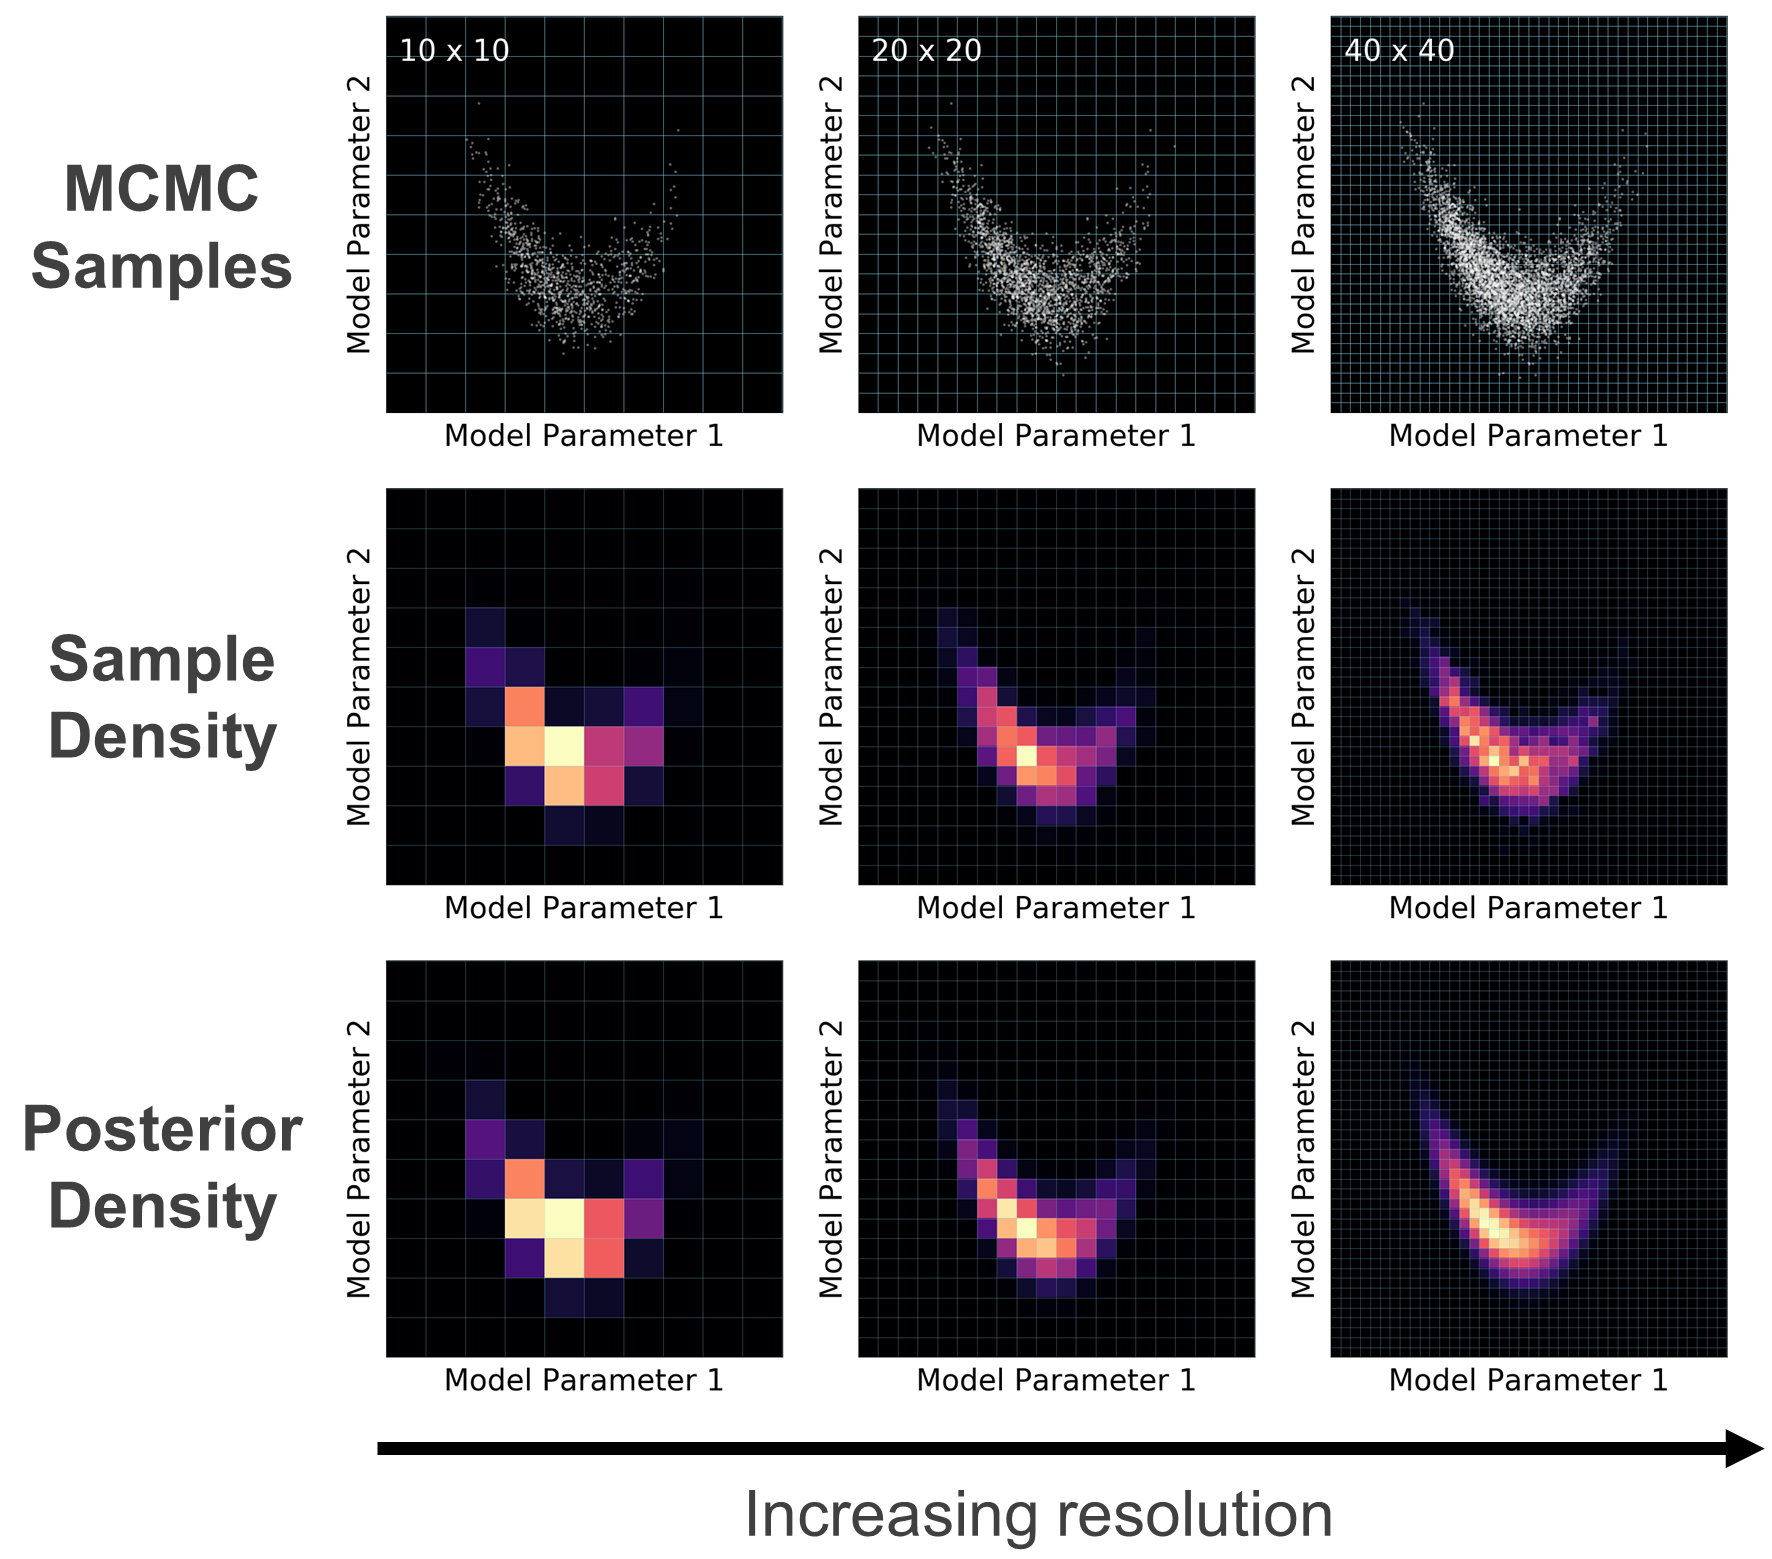
\includegraphics[width=\textwidth]{figures/fig8.png}
\end{center}
\caption{A schematic illustration of Markov Chain Monte Carlo (MCMC).
MCMC tries to create a chain of $n$ (correlated) samples 
$\{ \params_1 \rightarrow \dots \rightarrow \params_n \}$ (top)
such that the number of samples $m$ in some particular volume
$\delta$ gives a relative density $m/n$ (middle) comparable to the
posterior $\posterior(\params)$ integrated over the same volume (bottom).
See \S\ref{sec:mcmc} for additional details.
}\label{fig:mcmc}
\end{figure}

While this will just be approximately true for any finite $n$,
as the number of samples $n \rightarrow \infty$ this procedure generally
guarantees that $\rho(\params) \rightarrow \posterior(\params)$ 
everywhere.\footnote{Discussing the details of exactly when/where this
condition holds in theory and in practice
is beyond the scope of this paper but can be found in
other references such as \citet{asmussenglynn11} and \citet{brooks+11}.}
In theory then, once we have a reasonable enough
approximation for $\rho(\params)$, we can also use the 
samples $\{ \params_1 \rightarrow \dots \rightarrow \params_n \}$
generated from $\rho(\params)$
to get an estimate for the evidence using the 
same substitution trick introduced in \S\ref{sec:montecarlo}:
\begin{align}
    \evidence
    = \int \frac{\tilde{\posterior}(\params)}{\rho(\params)}
    \rho(\params) \deriv \params
    \equiv \meanwrt{\tilde{\posterior}(\params)/\rho(\params)}{\rho}
    \approx n^{-1} \sum_{i=1}^{n} 
    \frac{\tilde{\posterior}(\params_i)}{\rho(\params_i)}
\end{align}
This is just the average of the ratio 
between $\tilde{\posterior}(\params_i)$ and $\rho(\params_i)$
over all $n$ samples.

Finally, since our MCMC procedure gives us a series of $n$
samples from the posterior, our expectation value simply reduces to
\begin{equation}
    \meanwrt{f(\params)}{\posterior} 
    \approx \frac{n^{-1} \sum_{i=1}^{n} f_i \tilde{w}_i}
    {n^{-1} \sum_{i=1}^{n} \tilde{w}_i}
    = \frac{n^{-1} \sum_{i=1}^{n} f_i}
    {n^{-1} \sum_{i=1}^{n} 1}
    = n^{-1} \sum_{i=1}^{n} f_i
\end{equation}
This is just the \textbf{sample mean} of
the corresponding $\{ f_1, \dots, f_n \}$ values over
our set of $n$ samples. 

I wish to take a moment here to highlight two features of the above results
related to common misconceptions surrounding MCMC methods. First, there
is a widespread belief that because MCMC methods generate a chain of 
samples whose behavior \textit{follows} the posterior, we do not
have any ability to use them to estimate normalizing constants such
as the evidence $\evidence$. As shown above, this is not true at all: not only
\textit{can} we do this using $\rho(\params)$, but the estimate we derive
is actually a \textit{consistent} one (although it will converge slowly;
see \S\ref{subsec:post_approx}).

The second misconception is that the primary goal of MCMC is to
``approximate'' or ``explore'' the posterior. In other words,
to estimate $\rho(\params)$. However, as shown above,
the ability of MCMC methods to estimate $\rho(\params)$
is really only useful for estimating the evidence $\evidence$. In fact, by tracing
its heritage from Importance Sampling-based methods, we see its primary purpose
is actually \textit{to estimate expectation values} (i.e.
integrals \textit{over} the posterior). I have explicitly tried to avoid
introducing any mention of ``approximating the posterior'' up to this point
in order to avoid this misconception, but will spend some time discussing
this point in more detail in \S\ref{subsec:post_approx}.

To summarize, the idea behind MCMC is to simulate a series of
values $\{ \params_1 \rightarrow \dots \rightarrow \params_n \}$
in a way that their density $\rho(\params)$ after a given amount
of time follows the underlying posterior $\posterior(\params)$. We can
then estimate the posterior within any particular region $\delta_{\params}$
by simply counting up how many samples we simulate there and normalizing by
the total number of samples $n$ we generated. Because we are also
simulating values directly from the posterior, any expectation values
also reduce to simple sample averages. This procedure is incredibly
intuitive and part of the reason MCMC methods have 
become so widely adopted.

\subsection{Generating Samples with the Metropolis-Hastings Algorithm} \label{subsec:mh}

There is a vast literature on various approaches to generating samples
\textbf{(see, e.g., cites)}. Since this article focuses on
building up a \textit{conceptual understanding} of MCMC methods, 
exploring how the majority of these methods behave both in theory and
in practice is beyond the scope of this paper.

Instead of an overview, I aim to clarify the basics of how these methods operate.
The central idea is that we want a way to generate new samples 
$\params_i \rightarrow \params_{i+1}$ such that the
distribution of the final samples $\rho(\params)$ as $n \rightarrow \infty$
(1) is \textbf{stationary} (i.e. it converges to something) and 
(2) is equal to the $\posterior(\params)$. These are essentially analogs
to the convergence and consistency constraints 
discussed in \S\ref{subsec:consistent}.

We can satisfy the first condition by invoking \textbf{detailed balance}.
This is the idea that probability is conserved when moving
from one position to another (i.e. the process is reversible). More formally,
this just reduces to factoring of probability:
\begin{equation}
    P(\params_{i+1}|\params_i) P(\params_i) 
    = P(\params_{i+1}, \params_i)
    = P(\params_i|\params_{i+1}) P(\params_{i+1}) 
\end{equation}
where $P(\params_{i+1}|\params_i)$ is the probability of moving
from $\params_i \rightarrow \params_{i+1}$ and $P(\params_{i}|\params_{i+1})$ 
is the probability of the reverse move from 
$\params_{i+1} \rightarrow \params_i$. 
Rearranging then gives the following constraint:
\begin{equation}
    \frac{P(\params_{i+1}|\params_i)}{P(\params_i|\params_{i+1})} 
    = \frac{P(\params_{i+1})}{P(\params_i)}
    = \frac{\posterior(\params_{i+1})}{\posterior(\params_i)}
\end{equation}
where the final equality comes from the fact that the distribution
we are trying to generate samples from is the posterior $\posterior(\params)$.

We now need to implement a procedure that enables us to actually
move to new positions by computing this probability. 
We can do this by breaking each move into two steps. First,
we want to \textit{propose} a new position 
$\params_i \rightarrow \params_{i+1}'$ based on a
\textbf{proposal distribution} $\proposal(\params_{i+1}'|\params_i)$
similar in nature to the $\proposal(\params)$ used in to 
Importance Sampling (\S\ref{subsec:importance}). 
Then we will either decide to \textbf{accept} the new position
($\params_{i+1}=\params_{i+1}'$) or \textbf{reject} the new position
($\params_{i+1}=\params_i$) with some \textbf{transition probability}
$T(\params_{i+1}'|\params_i)$.
Combining these terms together then gives us the probability
of moving to a new position:
\begin{equation}
    P(\params_{i+1}|\params_i) 
    \equiv \proposal(\params_{i+1}|\params_i) T(\params_{i+1}|\params{i})
\end{equation}

As with Importance Sampling, we can choose $\proposal(\params_{i+1}'|\params_i)$
so that it is straightforward to propose new samples
$\params_{i+1}'$ by numerical simulation. 
We then need to determine the transition probability
$T(\params_{i+1}'|\params_i)$ of whether we should accept 
or reject $\params_{i+1}'$. Substituting into
our expression for detailed balance, we find that our form for the
transition probability must satisfy the following constraint:
\begin{equation}
    \frac{T(\params_{i+1}|\params_i)}{T(\params_i|\params_{i+1})} 
    = \frac{\posterior(\params_{i+1})}{\posterior(\params_i)}
    \frac{\proposal(\params_i|\params_{i+1})}{\proposal(\params_{i+1}|\params_i)}
\end{equation}
It is straightforward to show that the 
\textbf{Metropolis criterion} \cite{metropolis+53_alt}
\begin{equation}
    T(\params_{i+1}|\params_i)
    \equiv \min\left[1, \frac{\posterior(\params_{i+1})}{\posterior(\params_i)}
    \frac{\proposal(\params_i|\params_{i+1})}{\proposal(\params_{i+1}|\params_i)}
    \right]
\end{equation}
satisfies this constraint.

Generating samples following this approach can be done using the
\textbf{Metropolis-Hastings (MH) Algorithm} \citep{metropolis+53_alt,hastings70}:
\begin{enumerate}
    \item \textit{Propose} a new position $\params_i \rightarrow \params_{i+1}'$
    by generating a sample from the proposal distribution
    $\proposal(\params_{i+1}'|\params_i)$.
    \item \textit{Compute} the transition probability
    $T(\params_{i+1}'|\params_i)
    = \min\left[1, \frac{\posterior(\params_{i+1}')}{\posterior(\params_i)}
    \frac{\proposal(\params_i|\params_{i+1}')}{\proposal(\params_{i+1}'|\params_i)}
    \right]$.
    \item \textit{Generate} a random number $u_{i+1}$ from $[0, 1]$.
    \item If $u_{i+1} \leq T(\params_{i+1}'|\params_i)$, \textit{accept}
    the move and set $\params_{i+1} = \params_{i+1}'$. 
    If $u_{i+1} > T(\params_{i+1}'|\params_i)$, \textit{reject} the move
    and set $\params_{i+1} = \params_i$.
    \item Increment $i = i + 1$ and repeat this process.
\end{enumerate}
See {\color{red} \autoref{fig:mh}} for a schematic illustration of this process.

\begin{figure}
\begin{center}
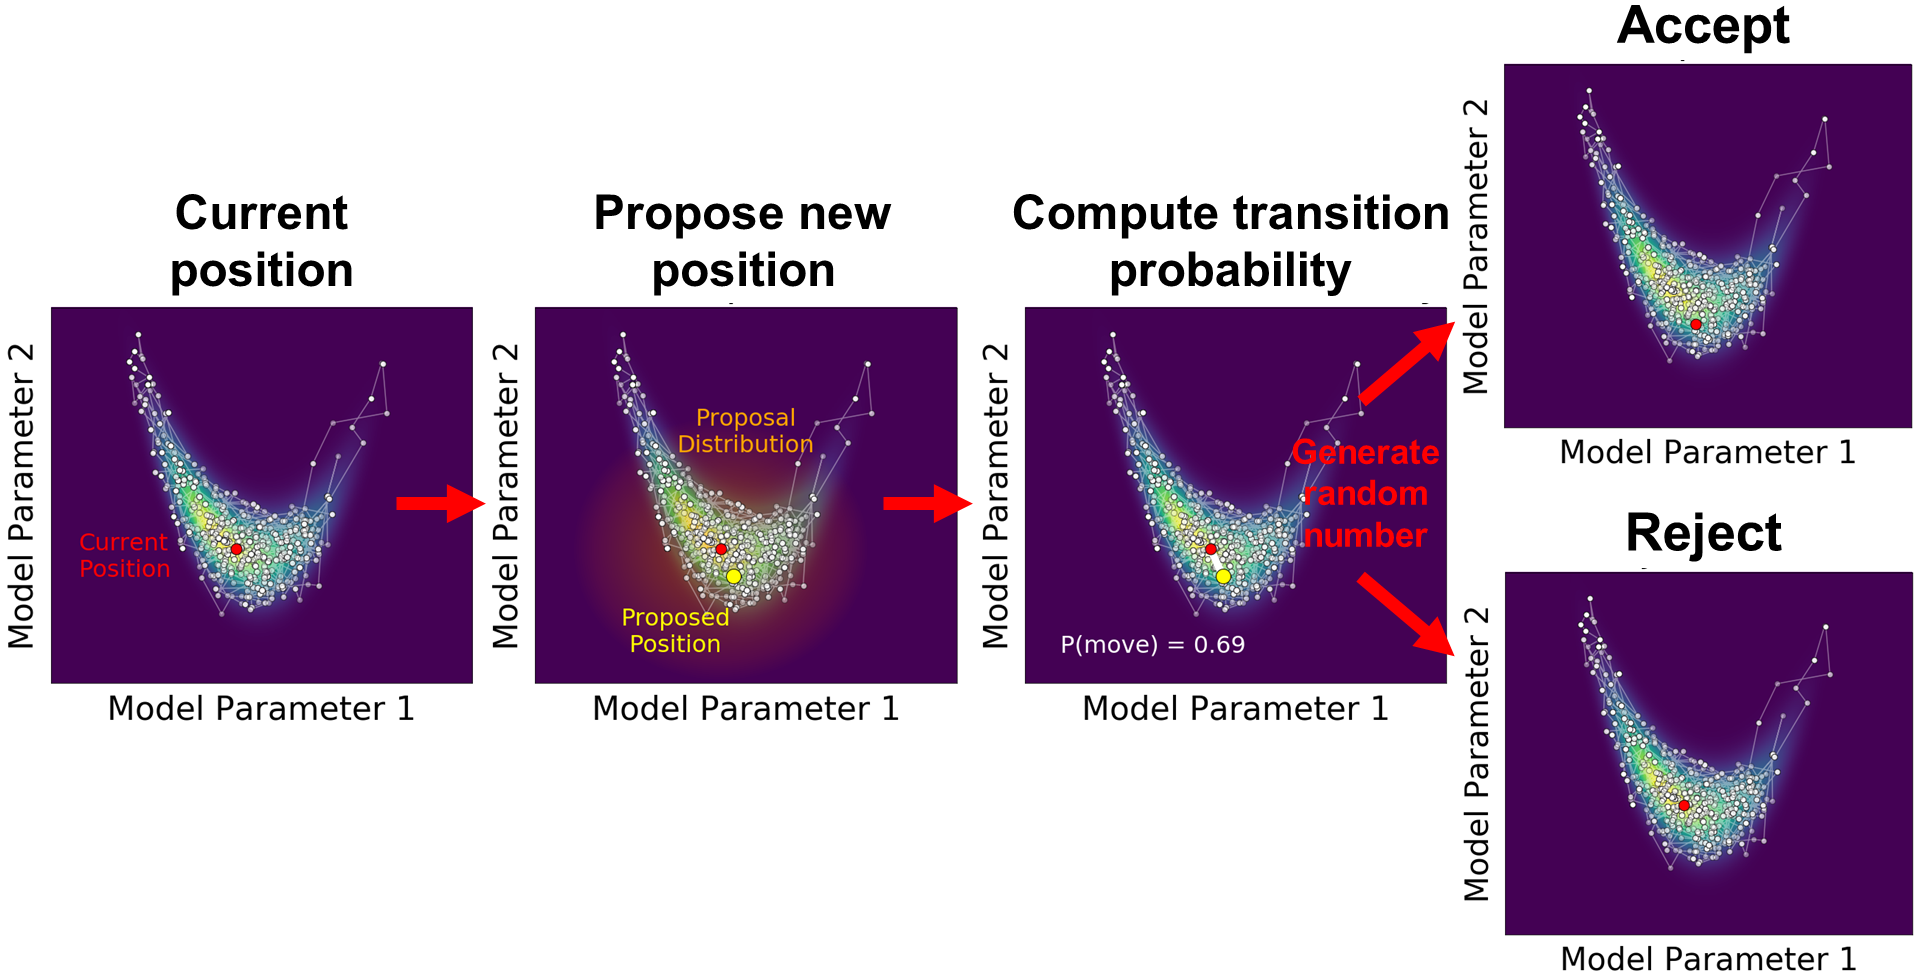
\includegraphics[width=\textwidth]{figures/fig10.png}
\end{center}
\caption{A schematic illustration of the Metropolis-Hastings
algorithm. At a given iteration $i$, we have generated a chain
of samples $\{ \params_1 \rightarrow \dots \rightarrow \params_i \}$
(white) up to the current position $\params_i$ (red) whose behavior follows
the underlying posterior $\posterior(\params)$ (viridis color map).
We then propose a new position $\params_{i+1}'$ (yellow) from the proposal distribution
(orange shaded region). We then compute 
the transition probability $T(\params_{i+1}'|\params_i)$
(white) based on the posterior $\proposal(\params)$ 
and proposal $\proposal(\params'|\params)$ densities. We then
generate a random number $u_{i+1}$ uniformly from 0 to 1. If
$u_{i+1} \leq T(\params_{i+1}'|\params_i)$, we accept the move
and make our next position in the chain $\params_{i+1} = \params_{i+1}'$.
If we reject the move, then $\params_{i+1} = \params_{i}$.
See \S\ref{subsec:mh} for additional details.
}\label{fig:mh}
\end{figure}

Because algorithms like the MH algorithm generate a \textit{chain} of states where the
next proposed position only depends on the current position rather than
any of its past positions (i.e. it ``forgets'' the past),
they are known as \textbf{Markov processes}.
Combining these two terms with the Monte Carlo nature of simulating new
positions is what gives Markov Chain Monte Carlo (MCMC) its namesake.

An issue with generating a chain of samples in practice is the
fact that our chain only has finite length and a starting position $\params_0$. 
If our chain were infinitely long, we would expect it
to visit every possible position in parameter space, rendering
the exact starting position is unimportant. However, since in practice we terminate 
sampling after only $n$ iterations, starting from a location $\params_0$ that has
an extremely low probability means an inordinate fraction
of our $n$ samples will occupy this low-probability region, possibly biasing
our final results. Since we have limited knowledge beforehand about where
$\params_0$ is relative to our posterior, 
in practice we generally want to remove the initial
chain of states once we are confident our chain has begun sampling from
higher-probability regions. Discussing various approaches
for identifying and removing samples from this \textbf{burn-in period} 
is beyond the scope of this article; for additional information,
please see \citet{gelmanrubin92}, \citet{gelman+13}, 
and \citet{vehtari+19} along with references therein.

\subsection{Effective Sample Size and Auto-Correlation Time} \label{subsec:autocorr}

At this point, MCMC seems like it should be the optimal method for
any situation: by simulating samples directly from the (unknown) posterior,
we can achieve an optimal estimate for any expectation values we wish
to evaluate. In practice, however, this does not hold true.
MCMC values rely on specific algorithmic procedures such as 
the MH algorithm to generate samples,
whose limiting behavior \textit{reduces to} a chain of samples
$\{ \params_1 \rightarrow \dots \rightarrow \params_n \}$
whose distribution follows the posterior. Any given sample $\params_i$,
however, is more likely than not to be 
\textbf{correlated} with both the previous sample in the 
sequence $\params_{i-1}$ and the subsequent sample in the sequence
$\params_{i+1}$.

This occurs for two reasons. First, new positions $\params_i$ drawn
from $\proposal(\params_i|\params_{i-1})$ by construction tend to depend
on the current position $\params_{i-1}$. This means that the position
we propose at iteration $i+1$ from will 
be correlated with the position at iteration $i$, 
which itself will be correlated with the position at
iteration $i-1$, etc. 

Second, even if we set
$\proposal(\params'|\params)=\proposal(\params')$ so that all
of our proposed positions are uncorrelated, 
our transition probability $T(\params'|\params)$ still ensures 
that we will eventually reject the new position 
so that $\params_{i+1}=\params_{i}$.
Since samples at exactly the same position are maximally correlated,
this ensures that samples from our chain will ``on average'' have non-zero
correlations. Note that having low \textbf{acceptance fractions} 
(i.e. the fraction of proposals that are accepted rather than rejected)
will lead to a larger fraction of the chain containing 
these perfectly correlated samples, increasing the overall correlation.

As mentioned in \S\ref{subsec:ess}, correlated samples
provide less information about the underlying distribution they
are sampled from since their behavior doesn't just depend on the
underlying distribution but also the neighboring samples in the
sequence. Samples that are more highly correlated then should 
lead to a reduced ESS.

This intuition can be quantified by introducing
the \textbf{auto-covariance} $C(t)$ 
for some integer lag $t$. Assuming that we have an infinitely long chain
$\{ \params_{1} \rightarrow \dots \}$,
the auto-covariance $C(t)$ is:
\begin{equation}
    C(t) \equiv \meanwrt{(\params_{i} - \bar{\params})
    \cdot (\params_{i+t} - \bar{\params})}{i}
    = \lim_{n\rightarrow\infty} \frac{1}{n}
    \sum_{i=1}^{n} (\params_{i} - \bar{\params}) \cdot (\params_{i+t} - \bar{\params})
\end{equation}
where $\cdot$ is the dot product. In other words, 
we want to know the covariance between $\params_i$ at some iteration
$i$ and $\params_{i+t}$ at some other iteration $i+t$, averaged
over all all possible pairs of samples $(\params_i, \params_{i+t})$
in our infinitely long chain. Note that the amplitude $|C(t)|$
will be maximized at $|C(t=0)|$,
where the two samples being compared are identical,
and minimized with $|C(t)|=0$ when 
$\params_{i}$ and $\params_{i+t}$ are completely independent
from each other.

Using the auto-covariance, we can define the corresponding
\textbf{auto-correlation} $A(t)$ as
\begin{equation}
    A(t) \equiv \frac{C(t)}{C(0)}
\end{equation}
This now measures the average degree of correlation between 
samples separated by an integer lag $t$. In the case where $t=0$,
both samples are identical and $A(t=0) = 1$. In the case
where the samples are uncorrelated over lag $t$,
$A(t) = 0$.

The overall \textbf{auto-correlation time}
for our chain is just the auto-correlation $A(t)$ summed over
all non-zero lags ($t \neq 0$):
\begin{equation}
    \tau \equiv \sum_{t=-\infty}^{\infty} A(t) - 1
    = 2 \sum_{t=1}^{\infty} A(t)
\end{equation}
where the $-1$ comes from the fact that
the auto-correlation with no lag is just $A(t=0) = 1$
(i.e. each sample perfectly correlates with itself) and
the substitution arises from the fact that $A(t) = A(-t)$ by symmetry.
If $\tau = 0$, then it takes
no time at all for samples to become uncorrelated and the
samples can be assumed to be iid. If $\tau > 0$, then
it takes on average $\tau$ additional iterations for
samples to become uncorrelated. 
An illustration of this process is shown in 
{\color{red} \autoref{fig:autocorr}}.

\begin{figure}
\begin{center}
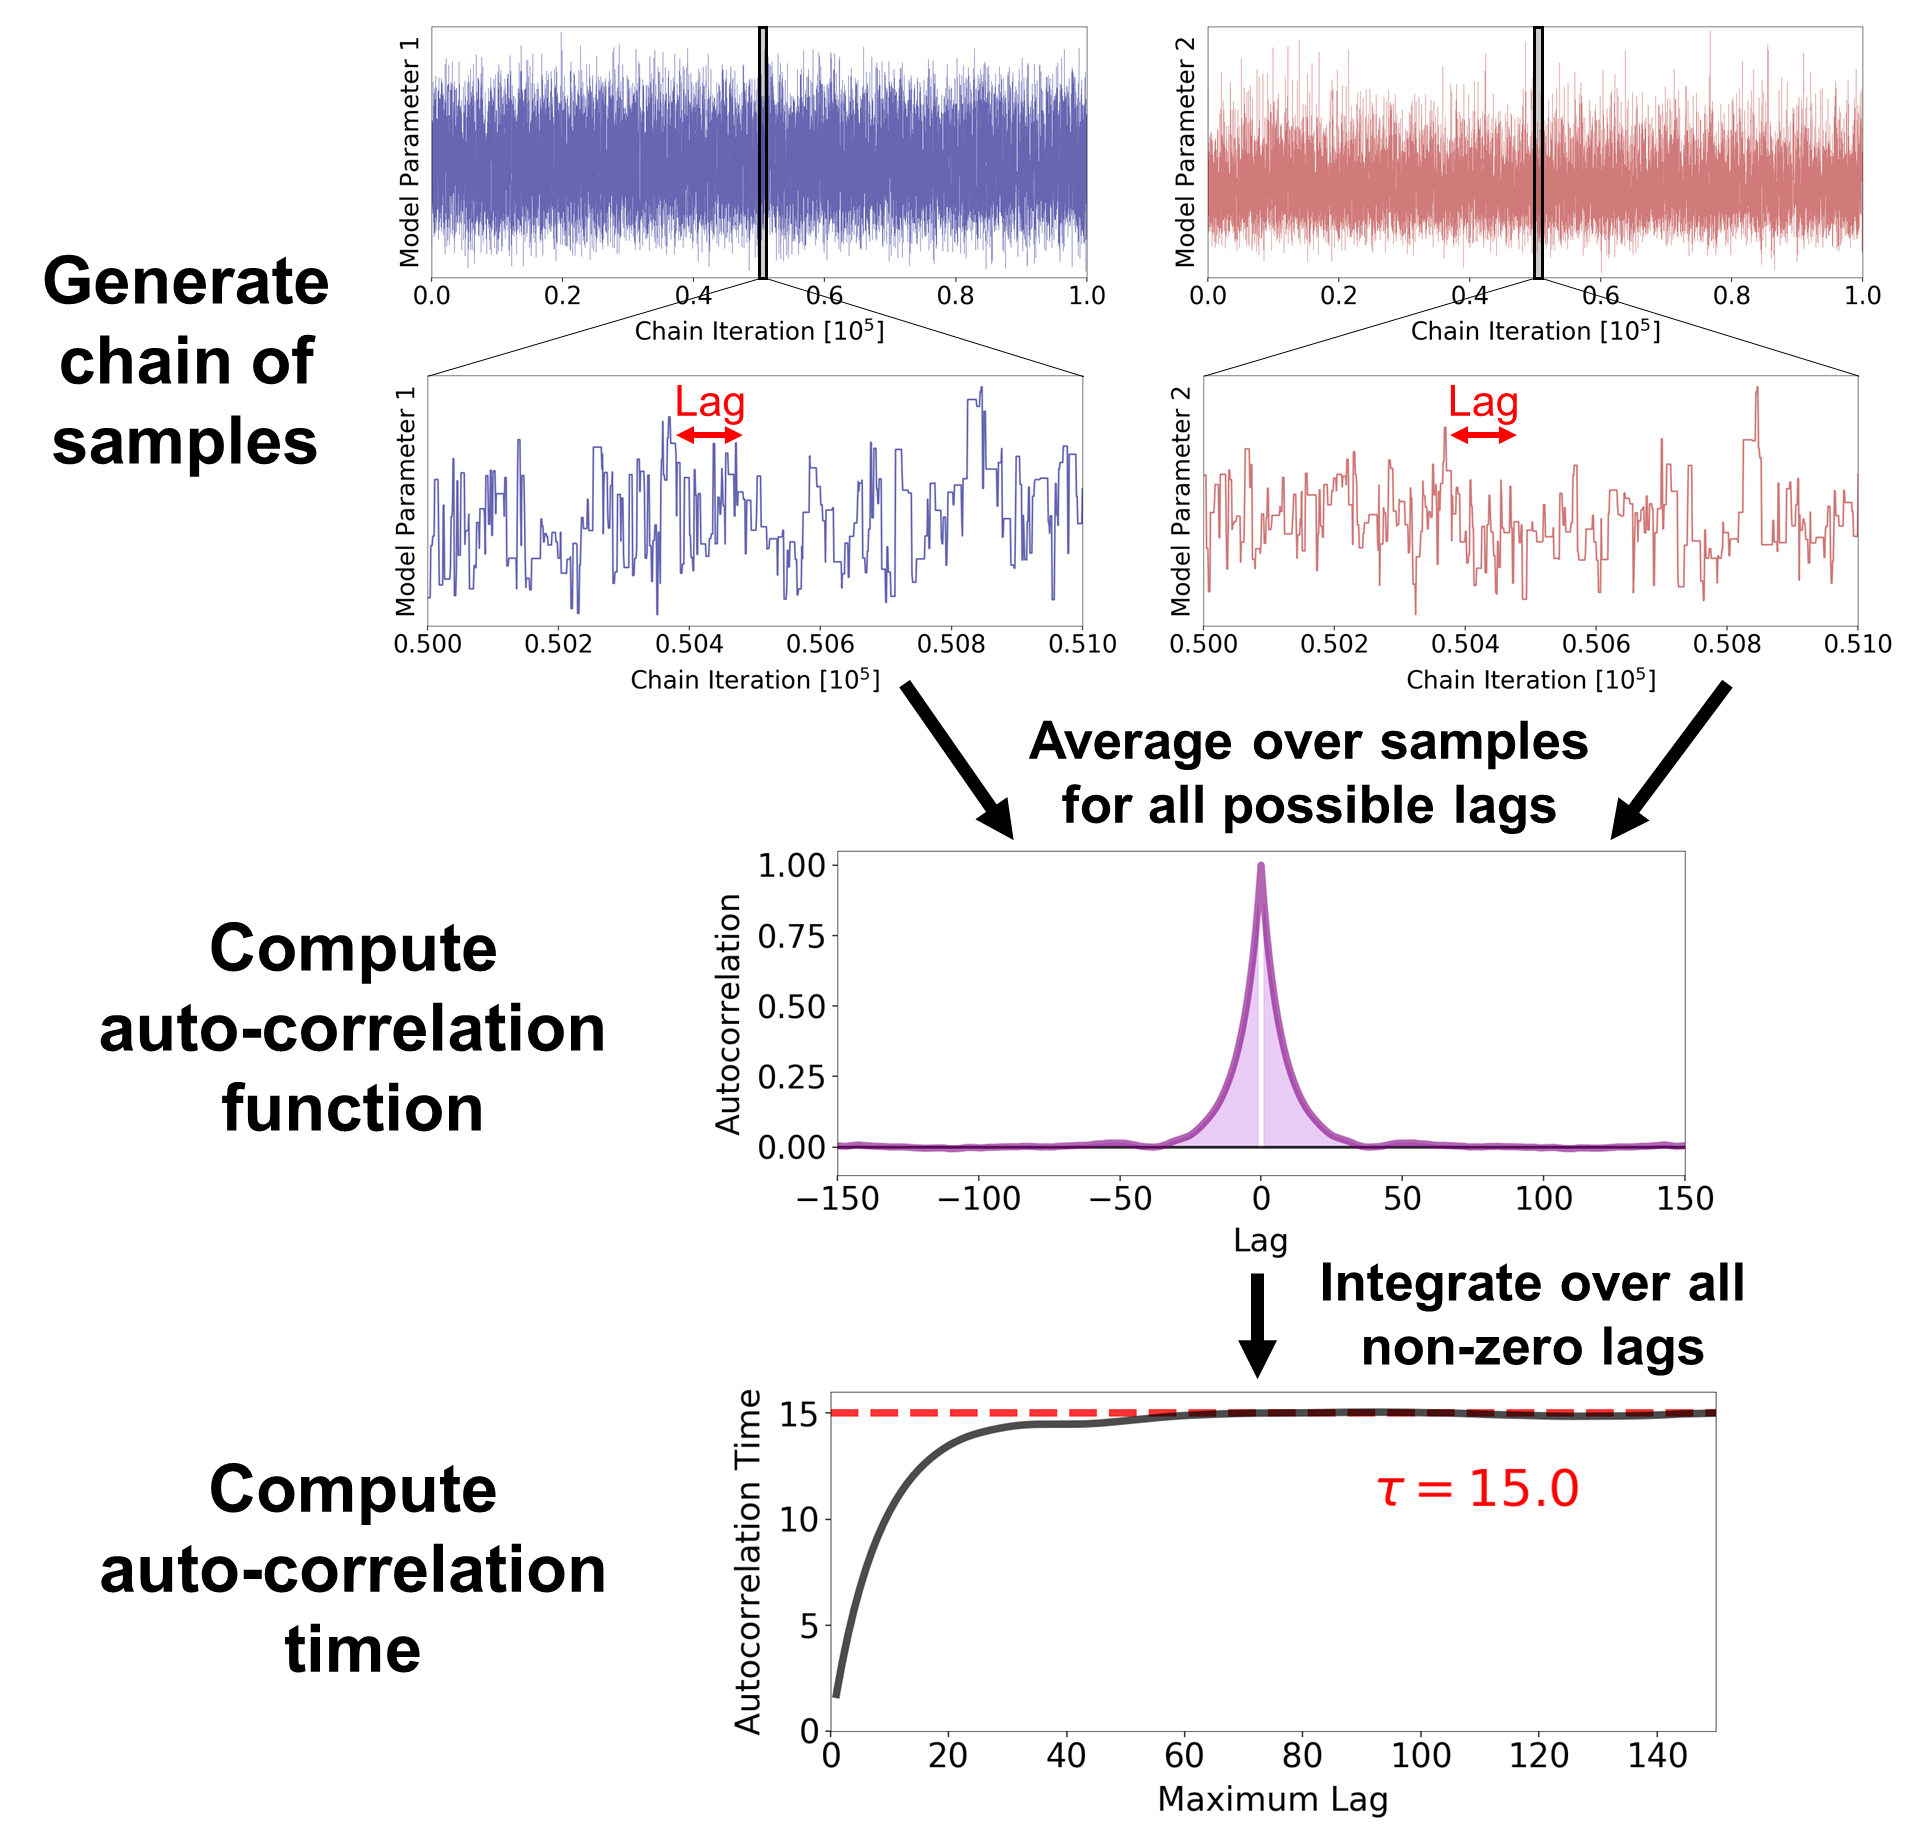
\includegraphics[width=\textwidth]{figures/fig9.png}
\end{center}
\caption{A schematic illustration of the auto-correlation
associated with MCMC. MCMC methods generate a chain of
samples $\{ \params_1 \rightarrow \dots \rightarrow \params_n \}$ (top),
but these tend to be strongly correlated on small length scales (top middle).
We can quantify the degree of correlation by
computing the corresponding auto-correlation $A(t)$
over our set of samples and all possible time lags $t$
(bottom middle). This quantity is $1$ when $t=0$
and drops to $0$ as $t \rightarrow \pm \infty$. The overall
auto-correlation time $\tau$ associated with our chain of
samples is then just the integrated auto-correlation over $t \neq 0$.
See \S\ref{subsec:autocorr} for additional details.
}\label{fig:autocorr}
\end{figure}

Incorporating the auto-correlation time leads directly
to a modified definition for the ESS:
\begin{equation}
    n_{\rm eff}' \equiv \frac{n_{\rm eff}}{1 + \tau}
\end{equation}
In practice, we cannot precisely compute $\tau$ since
we do not have an infinite number of samples and do not know
$\posterior(\params)$. Therefore we often need to
generate an estimate $\hat{\tau}$ of the auto-correlation time
using the existing set of $n$ samples we have. While discussing
various approaches taken to derive $\hat{\tau}$ is beyond the
scope of this work, please see \citet{brooks+11} 
for additional details.

The fact that MCMC methods are subject to non-negative
auto-correlation times ($\tau \geq 0$) but have optimal importance
weights $\tilde{w}_i = 1$ give an ESS of
\begin{equation}
    n_{\rm eff,MCMC}' = \frac{n_{\rm eff,MCMC}}{1 + \tau}
    = \frac{n}{1 + \tau} \leq n
\end{equation}
This means that \textit{there is no guarantee
that MCMC is always the optimal choice to achieve
the largest ESS}. In particular,
Importance Sampling methods, which can generate
fully iid samples with no auto-correlation time ($\tau = 0$)
but non-optimal importance weights $\tilde{w}_i$, instead have
an ESS of
\begin{equation}
    n_{\rm eff,IS}' = \frac{n_{\rm eff,IS}}{1 + \tau}
    = n_{\rm eff,IS} 
    = \frac{\left(\sum_{i=1}^{n} \tilde{w}_i\right)^2}
    {\sum_{i=1}^{n} \tilde{w}_i^2} \leq n
\end{equation}
which can be greater than $n_{\rm eff, MCMC}'$ at fixed $n$.

Given the results above, it should now be clear
that \textit{the central motivating concern of MCMC methods
is whether they can generate a chain of samples
with an auto-correlation time small enough to outperform
Importance Sampling.} Whether or not
this is true will depend on the posterior, the approach used to generate
the chain of samples (see \S\ref{subsec:mh} and \S\ref{sec:example})
and the proposal distribution $\proposal(\params)$ 
used for Importance Sampling (see \S\ref{subsection:samp_strat}).

\subsection*{Exercise: MCMC over a 2-D Gaussian} \label{exercise:mcmc}

\subsubsection*{Setup}

Let's again return to our examples from 
\S\ref{sec:grid} and \S\ref{sec:montecarlo}, in which
our unnormalized posterior is well-approximated by a 2-D Gaussian (Normal)
distribution:
\begin{equation*}
    \tilde{\posterior}(x,y) 
    = \exp\left\{-\frac{1}{2}\left[\frac{(x-\mu_x)^2}{\sigma_x^2}
    + \frac{(y-\mu_y)^2}{\sigma_y^2}\right]\right\}
\end{equation*}
where $(\mu_x,\mu_y)=(-0.3,0.8)$ and $(\sigma_x^2,\sigma_y^2)=(2,0.5)$.

We want to use MCMC to approximate various posterior
integrals from this distribution.
We will start by choosing our proposal distribution $\proposal(x',y'|x,y)$
to be a 2-D Gaussian with a mean of $0$ and standard deviation of $1$:
\begin{equation*}
    \proposal(x',y'|x,y) = \Normal{(\mu_x,\mu_y)=(x,y)}{(\sigma_x,\sigma_y)=(1,1)}
\end{equation*}

\subsubsection*{Parameter Estimation}

Using the above proposal, generate $n=1000$ samples following the MH algorithm starting
from the position $(x_0,y_0)=(0,0)$. Using these samples,
compute an estimate of the means $\meanwrt{x}{\posterior}$
and $\meanwrt{y}{\posterior}$ as well as the corresponding 68\% credible
intervals (or closest approximation)
$[x_{\rm low}, x_{\rm high}]$ and $[y_{\rm low}, y_{\rm high}]$.
How accurate are each of these quantities compared with the values we might
expect?

\subsubsection*{Evidence Estimation}

Next, use a set of $10 \times 10$ bins from
$x=[-5, 5]$ and $y=[-5, 5]$ to construct an estimate $\rho(x,y)$ 
from the resulting set of samples. Using this estimate
for the density, compute an estimate of the evidence $\evidence$.
How accurate is our approximation? Does it substantially
change if we adjust the number and/or size of the bins?

\subsubsection*{Auto-Correlation Time and Effective Sample Size}

Use numerical methods to compute an estimate of the
auto-correlation time $\tau$ and the corresponding effective sample size $n_{\rm eff}$.
How efficient is our sampling ($n_{\rm eff}/n$) compared to the default
Importance Sampling approach from the exercise in \S\ref{sec:montecarlo}?
Does this mirror what we'd expect given the acceptance fraction of our proposals?
What do these quantities this tell us about how well 
our proposal $\proposal(x,y)$ matches the structure of the underlying posterior
$\posterior(x,y)$?

\subsubsection*{Uncertainties}

Repeat the above exercises $m=30$ times to get an
estimate for how much our estimates of each quantity can vary.
Is the variation in line with what might be expected given 
the typical effective sample size?

\subsubsection*{Consistency and Convergence}

Now repeat the above exercise using $n=2500$ and $n=10000$ samples
points and comment on any differences.
How much has the overall accuracy improved? Do
the estimates appear convergent and consistent as $n_{\rm eff}$ increases? 
How much do the errors on quantities shrink as a function 
of $n$ and/or $n_{\rm eff}$? Is this similar or different
from the observed dependence from the Importance Sampling exercise
in \S\ref{sec:montecarlo}?

\subsubsection*{Sampling Efficiency}

Next, adjust the $(\sigma_x, \sigma_y)$ of the proposal distribution
to try and improve $n_{\rm eff}$ at fixed $n$. How close is the final
ratio $\sigma_x/\sigma_y$ of our proposal to that of the underlying
posterior? Are there any additional scaling differences between the rough
size of our proposal $\proposal(x',y'|x,y)$ relative to the
underlying posterior $\posterior(x,y)$?
Given that $\tilde{\posterior}(x,y)$ may differ from the
structure assumed when picking $\proposal(x',y'|x,y)$,
can you think of any possible scheme to try and adjust our proposal
using an existing set of samples?

\subsubsection*{Burn-In}

Finally, adjust the starting position to be at
$(x_0,y_0)=(10,10)$ instead of $(0,0)$ and generate a new chain of 
samples. Plot the $x$ and $y$ positions of the chain over time.
Are there any obvious signs of the burn-in period? How many samples
roughly should be assigned to burn-in and subsequently removed from
our chain? Are there any possible heuristics that might help to identify
the initial burn-in period?

\section{Sampling the Posterior with MCMC} \label{sec:sampling}

The approach by which MCMC methods are able to generate a chain of
samples immediately gives a mental image of our chain ``exploring'' the
posterior. While it is true that the density of samples from the chain
$\rho(\params) \rightarrow \posterior(\params)$ as $n \rightarrow \infty$, 
\textit{the primary purpose of MCMC is estimating expectation values}
$\meanwrt{f(\params)}{\posterior}$.
Although this might seem like a subtle difference,
this distinction is actually crucial for understanding how MCMC
algorithms (should) behave in practice. We discuss this in more
detail below.

\subsection{Approximating the Posterior} \label{subsec:post_approx}

Although algorithms such as MH (\S\ref{subsec:mh}) are constructed to
ensure the density of the chain of samples $\rho(\params)$
generated by MCMC converges to the posterior $\posterior(\params)$
as $n \rightarrow \infty$, this \textit{does not} necessarily translate
into an efficient method to approximate the posterior in practice. In
other words, $n$ might need to be extremely large for this constraint to hold.
So how many samples do we need to ensure $\rho(\params)$ is a good approximation
to $\posterior(\params)$?

To start, we first need to define some metric for what a ``good''
approximation is. A reasonable one might be that we would like
to know the posterior within some region $\delta_{\params}$
to within some precision $\epsilon$ so that
\begin{equation}
    \left| \frac{1}{n} \sum_{i=1}^{n} \indicator{\params_i \in \delta_{\params}} 
    - \int_{\delta_{\params}} \posterior(\params) \deriv \params \right|
    \equiv |\hat{p}(\delta_{\params}) - p(\delta_{\params})| < \epsilon
\end{equation}
where $p(\delta_{\params})$ is the total probability contained within
$\delta_{\params}$ and $\hat{p}(\delta_{\params})$ is the fraction of
the MCMC chain of samples contained within the same region. While it might
seem strange to only estimate this for one region, I will shortly
generalize this to encompass the
entire\footnote{Technically the procedure outlined in this section
only works for finite volumes. The basic intuition, however, holds even
when parameters are unbounded although proving those results is beyond
the scope of this work.} posterior.

In the ideal case where our samples are iid and drawn from $\posterior(\params)$,
our samples each have a probability $p(\delta_{\params})$ 
of being within $\delta_{\params}$.
The probability that $\hat{p}(\delta_{\params}) = m/n$ then follows the
\textbf{binomial distribution}:
\begin{equation}
    P\left(\hat{p}(\delta_{\params}) = \frac{m}{n} \right) 
    = \binom{n}{m} \left[p(\delta_{\params})\right]^m
    \left[1 - p(\delta_{\params}) \right]^{n-m}
\end{equation}
In other words, our samples end up inside $\delta_{\params}$ a total of $m$ times
with probability $p(\delta_{\params})$ and outside $\delta_{\params}$ a
total of $n-m$ times with probability $1 - p(\delta_{\params})$. The
additional binomial coefficient $\binom{n}{m}$ for ``$n$ choose $m$'' 
accounts for all possible unique cases where $m$ samples can
end up within $\delta_{\params}$ out of our total sample size of $n$.

This distribution has a mean of $p(\delta_{\params})$, so for
any finite $n$ we expect $\hat{p}(\delta_{\params})$ to be an
\textbf{unbiased estimator} of $p(\delta_{\params})$:
\begin{equation}
    \mean{\hat{p}(\delta_{\params}) - p(\delta_{\params})} 
    = p(\delta_{\params}) - p(\delta_{\params}) = 0
\end{equation}
The variance, however, depends on the sample size:
\begin{equation}
    \mean{|\hat{p}(\delta_{\params}) - p(\delta_{\params})|^2}
    = \frac{p(\delta_{\params}) \left[1 - p(\delta_{\params})\right]}{n}
\end{equation}

In practice, we can expect there to be some non-zero auto-correlation
time $\tau > 0$. This will increase the number of MCMC samples
we will need to generate to be confident that our estimate
$\hat{p}(\delta_{\params})$ is well-behaved. Inserting a factor
of $1+\tau$ and substituting our expectation value from above
into our accuracy constraint then gives a
rough constraint for the number of samples $n$ we would require
as a function of $\epsilon$:
\begin{equation}
    n \gtrsim 
    \frac{p(\delta_{\params}) \left[1 - p(\delta_{\params})\right]}
    {\epsilon^2/(1+\tau)} 
    \sim \frac{\hat{p}(\delta_{\params}) 
    \left[1 - \hat{p}(\delta_{\params})\right]}
    {\epsilon^2} \times (1+\hat{\tau})
\end{equation}
The final substitution of $p(\delta_{\params})$ and $\tau$ with their
noisy estimates $\hat{p}(\delta_{\params})$ and $\hat{\tau}$
arises from the fact that
in practice we don't know $p(\delta_{\params})$ or 
$\tau$ (both of which require full knowledge of the posterior).
We are therefore forced to rely on estimators
derived from our set of $n$ samples.

Let's now examine this result more closely. As expected,
the total number of samples is proportional
to $1 + \hat{\tau}$: if it takes longer to generate independent
samples, then we need more samples to be confident we have characterized
the posterior well in a given region. 
We also see that $n \propto \epsilon^{-2}$, so that
if we want to reduce the error by a factor of $x$ we need
to increase our sample size by a factor of $x^2$.

The behavior in the numerator is more interesting. Note
that $\hat{p}(\delta_{\params}) \left[1 - \hat{p}(\delta_{\params})\right]$
is maximized for $\hat{p}(\delta_{\params}) = 0.5$, and so the largest
sample size needed is when we have split our posterior directly in half.
In all other cases the sample size needed will be smaller because
there will be more samples outside or inside the region of interest
whose information we can leverage. The exact value of $\hat{p}(\delta_{\params})$
of course depends on both the posterior $\posterior(\params)$
and the target region $\delta_{\params}$: the sample size needed to approximate
the posterior to some $\epsilon$ 
near the peak of the distribution (the small region where $\posterior(\params)$ is large)
will likely be different than
the sample size needed to accurately estimate the tails of the
distribution (the large region where $\posterior(\params)$ is small).

While the above argument holds if we are looking to estimate the
posterior in just \textit{one} region, ``converging to the posterior''
implies that we want $\rho(\params)$
to become a good approximation to $\posterior(\params)$ \textit{everywhere}.
We can enforce this new requirement by splitting our posterior into $m$
different sub-regions $\{ \delta_{\params_1}, \dots, \delta_{\params_m} \}$ 
and requiring that each sub-region is well constrained:
\begin{equation}
    |\hat{p}(\delta_{\params_1}) - p(\delta_{\params_1})| < \epsilon_1
    \quad\quad \dots \quad\quad
    |\hat{p}(\delta_{\params_m}) - p(\delta_{\params_m})| < \epsilon_m
\end{equation}
Substituting in the expected errors on each of these
constraints then gives us an approximate limit
on the number of samples $n_j$ that we need
to estimate the posterior in each region $\delta_{\params_j}$:
\begin{equation}
    n_j \gtrsim \frac{\hat{p}(\delta_{\params_j}) 
    \left[1 - \hat{p}(\delta_{\params_j})\right]}
    {\epsilon_j^2} \times (1+\hat{\tau})
\end{equation}
The total number of samples we need is then simply:
\begin{equation}
    n \gtrsim 
    \sum_{j=1}^{m} n_j
\end{equation}

This approach of dividing up our posterior into sub-regions
is conceptually similar to the grid-based approaches
described in \S\ref{sec:grid}. As such,
it is also subject to the same drawbacks:
we expect the number of regions $m$ to increase
\textit{exponentially} with the number of dimensions $d$.
For instance, if we just wanted to divide our posterior up
into $m$ \textbf{orthants} we would end up with $m=2^d$ regions:
2 in 1-D (left-right), 4 in 2-D (upper-left, lower-left,
upper-right, lower-right), 8 in 3-D, etc.

This effect implies that we should in general expect
the number of samples required to ensure $\rho(\params)$ is a good
approximation to $\posterior(\params)$ for some specified accuracy $\epsilon$
to scale as
\begin{equation}
    n \gtrsim k^d
\end{equation}
where $k$ is a constant that depends on the accuracy requirements.
This puts approximating the full posterior firmly in the 
``curse of dimensionality'' regime (see \S\ref{subsec:curse}).\footnote{
A direct corollary of this result is that, while the
evidence estimates from MCMC \textit{are} consistent, 
the rate of convergence to the underlying value 
will proceed exponentially more slowly
as $d$ increases.}

While many practitioners talk about MCMC being 
an efficient method to ``approximate the posterior'', in practice it is rarely
used to approximate $\posterior(\params)$ directly.
As discussed in \S\ref{sec:what} and shown in
{\color{red} \autoref{fig:corner}}, almost all quantities 
that are reported in the literature \textit{do not} rely on approximations to
the full $d$-dimensional posterior, but rather approximations to marginalized
distributions that are almost always restricted to no more 
than $k\lesssim3$ parameters at a time.
The act of marginalizing over the remaining $d-k$ parameters
helps to counteract the curse of dimensionality illustrated here.
While it is technically fair to say that MCMC can ``explore'' 
the marginalized $k$-D posteriors for certain limited sets of parameters, 
this type of language can often lead to more misconceptions than insights.

\subsection{Posterior Volume} \label{subsec:volume}

The basic consequences outlined in \S\ref{subsec:post_approx} 
are more general than the specific case where we imagine dividing
up the posterior into orthants or other regions.
Fundamentally, computing any expectation
over the posterior $\meanwrt{f(\params)}{\posterior}$ requires
integrating over the \textit{entire domain} of our parameters 
$\params$. We therefore want to understand how the \textbf{volume}
of this domain behaves (i.e. how many parameter combinations there are).
Once we have a grasp on how this behaves, we can then starting trying
to quantify how this will impact our estimates.
%  for the posterior
% $\posterior(\params)$ versus expectation values over the posterior
% $\meanwrt{f(\params)}{\posterior}$

To start, let's consider the
$d$-dimensional hyper-cube (the $d$-cube)
with side length $\ell$ in all $d$ dimensions. Its volume scales as
\begin{equation}
    V(\ell) = \prod_{i=1}^{d} \ell = \ell^d
\end{equation}
The differential volume element between $\ell$ and
$\ell + \deriv \ell$ is
\begin{equation}
    \deriv V(\ell) = (d \times \ell^{d-1}) \times (\deriv\ell) \propto \ell^{d-1}
\end{equation}

This exponential scaling with dimensionality means that volume becomes
increasingly concentrated in thin shells located in regions located
progressively further away from the center of the $d$-cube. 
As an example, consider the length-scale
\begin{equation}
    \ell_{50} = 2^{-1/d} \ell
\end{equation}
that divides the $d$-cube into two equal-sized regions
with 50\% of the volume contained interior to $\ell_{50}$ and
50\% of the volume exterior to $\ell_{50}$. 
In 1-D, this gives $\ell_{50}/\ell = 0.5$ as we'd
expect. In 2-D, this gives $\ell_{50}/\ell \approx 0.7$. In 3-D,
$\ell_{50}/\ell \approx 0.8$. In 7-D, $\ell_{50}/\ell \approx 0.9$.
By the time we get to 15-D, we have $\ell_{50} /\ell\approx 0.95$,
which means that 50\% of the volume is located in the last 5\% of the 
length-scale near the boundary of the $d$-cube.
While the constants may change when considering other shapes (e.g., spheres),
in general this exponential scaling as a function of $d$ is a generic feature
of higher-dimensional volumes. In other words, increasing the number
of parameters leads to an exponential increase in the number of
available parameter combinations that we have to explore.

\begin{figure}
\begin{center}
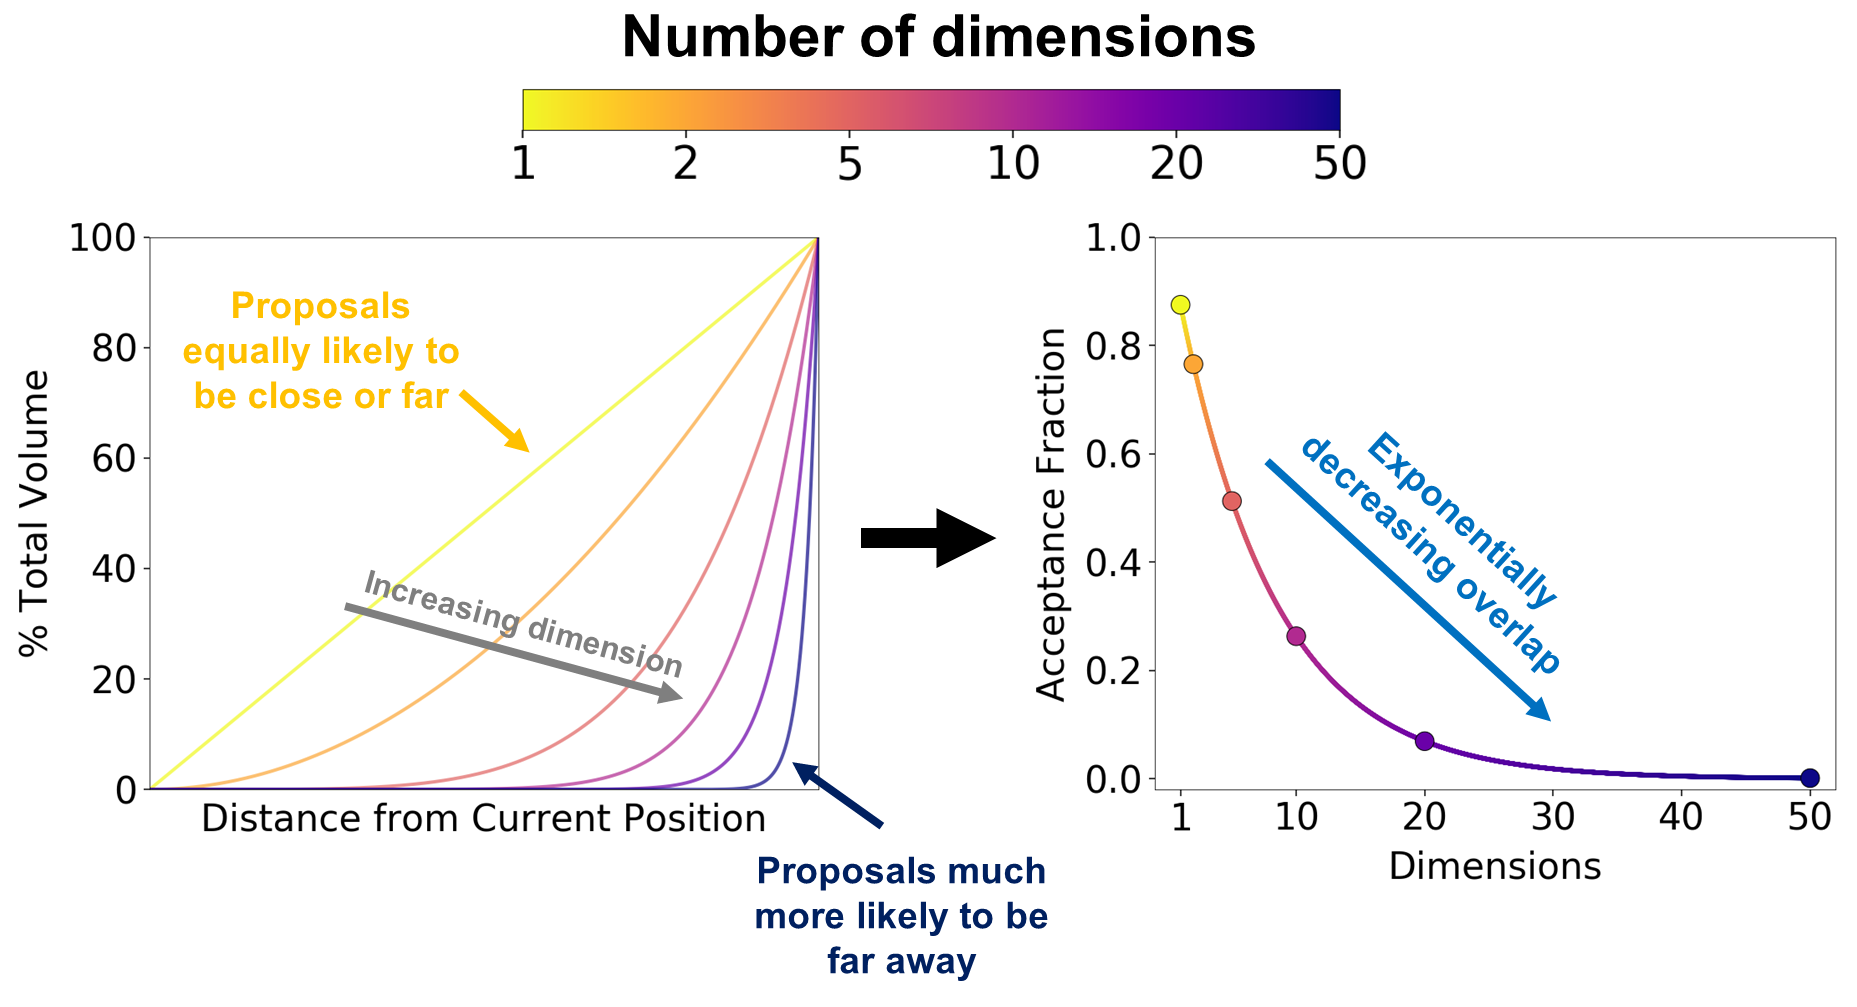
\includegraphics[width=\textwidth]{figures/fig11.png}
\end{center}
\caption{A schematic illustration of how the curse of dimensionality
affects MCMC acceptance fractions via posterior volume.
At a given position position $\params$, 
the volume increases $\propto r^d$ as a function 
of distance $r$ away from that position (left). 
As the dimensionality increases, this implies volume
becomes concentrated progressively further out, leading to 
larger distances between proposed positions $\params'$ and the current
position $\params$. Most of these positions have significantly lower
posterior probabilities $\posterior(\params')$ compared to the 
current value $\posterior(\params)$, leading to an
exponential decline in the typical acceptance fraction
(and a corresponding increase in the auto-correlation time)
as the dimensionality increases (right). Adjusting the size
and/or shape of the proposal $\proposal(\params'|\params)$
can help to counteract this behavior.
See \S\ref{subsec:volume} for additional details.
}\label{fig:vol}
\end{figure}

In addition to affecting the long-term behavior of MCMC, 
this exponential increase in volume also directly
impacts how MCMC methods operate. To see why this is the case, we
need look no further than the transition probability used in the
MH algorithm discussed in \S\ref{subsec:mh}:
\begin{equation*}
    T(\params_{i+1}|\params_i)
    \equiv \min\left[1, \frac{\posterior(\params_{i+1})}{\posterior(\params_i)}
    \frac{\proposal(\params_i|\params_{i+1})}{\proposal(\params_{i+1}|\params_i)}
    \right]
\end{equation*}
The non-trivial portion of this expression cleanly splits into two terms.
The first is dependent on the \textit{volume} and is related to
how we proposed our next position from $\proposal(\params'|\params)$.
The second is dependent on the \textit{density} and is related to
how the posterior density changes between the two positions.

In practice, our transition probability can be interpreted as
a basic corrective approach: after proposing
a new position from some nearby volume, we then try to ``correct''
for differences between our proposal and the underlying posterior
by only accepting these moves sometimes based on changes in the underlying density.
In high dimensions, this basic ``tug of war'' between the volume (proposal) and
the density (posterior) can break down as the vast majority of an object's 
volume becomes concentrated near the outer edges.\footnote{Alternative
methods such as Hamiltonian Monte Carlo \citep{neal12} can get around
this problem by smoothly incorporating changes in the density and volume.}
For instance, in the case where our
proposal $\proposal(\params'|\params)$ is a cube with side-length $\ell$
centered on $\params$, this leads to a median length-scale of
$\ell_{50} = 2^{-1/d} \ell$, which increases rapidly from $0.5 \ell$
to $\approx \ell$ as the dimensionality increases. The same logic
also applies to other proposal distributions (see \S\ref{sec:example}).
This focus on positions either far away or with very similar separation
length-scales as $\ell_{50} \rightarrow \ell$ 
means that many choices of $\proposal(\params'|\params)$
have a tendency to ``overshoot'', proposing new positions with much
smaller posterior densities compared to the current position. These
new positions are then almost always rejected, leading to extremely
low acceptance fractions and correspondingly
long auto-correlation times. An example of this effect is
illustrated in {\color{red} \autoref{fig:vol}.}

One of the main ways to counteract this behavior is to
adjust the size/shape of the proposal $\proposal(\params'|\params)$
so that the fraction of proposed positions that are accepted remains
sufficiently high. This helps to ensure the posterior density 
$\posterior(\params)$ does not change too drastically when proposing 
positions new positions, leading to lower overall auto-correlation times.
Details of how to implement these schemes in practice are beyond 
the scope of this article; please see
\textbf{citation} for additional details.

\subsection{Posterior Mass and Typical Sets} \label{subsec:mass}

Above, I described how the behavior of volume in high dimensions
can impact the performance of our MCMC MH sampling algorithm,
possibly leading to inefficient proposals and 
low acceptance fractions. Let's assume that we have resolved this
problem and have an efficient way of generating our chain
of samples. We now have a secondary question: \textit{where are these
samples located?}

From our discussion in \S\ref{subsec:post_approx}, we know that
the highest \textit{density} of samples $\rho(\params)$
will be located where the posterior density $\posterior(\params)$
is also correspondingly high. However, this region $\delta_{\params}$
might only correspond to a small portion of the posterior. 
Indeed, given there is exponentially more volume as the dimensionality
increases, it is almost guaranteed that models with many parameters
$\params$ will have the vast majority of the posterior located
outside the region of highest density. 

A consequence of this is that
the majority of samples in our chain will be located
away from the peak density. As a result, \textit{our chain
spends the majority of its time
generating samples in these regions}.
This has a huge impact in the way our chain is expected to behave:
while the highest \textit{concentration}
of samples will be located in the regions of highest
posterior density, the largest \textit{amount} of samples
will actually be located in the regions of highest \textbf{posterior
mass} (i.e. density times volume). 
Since this implies that a ``typical'' sample 
(picked at random) will most likely be located in this
region of high posterior mass,
this region is also commonly referred to
as the \textbf{typical set}.

To make this argument a little easier to conceptualize,
let's imagine that we have a 3-parameter model $\params = (x, y, z)$ 
and $\posterior(x,y,z)$ is spherically symmetric.
While we could imagine trying to
integrate over $\posterior(x,y,z)$ directly in terms of
$\deriv x \deriv y \deriv z$, it is almost always
easier to instead integrate over such a distribution
in ``shells'' with differential volume
$\deriv V(r) = 4 \pi r^2 \deriv r$
as a function of radius
$r = \sqrt{x^2 + y^2 + z^2}$. This allows us
to rewrite the 3-D integral over $(x,y,z)$ as a 1-D integral over $r$:
\begin{equation}
    \int \posterior(x,y,z) \deriv x \deriv y \deriv z
    = \int \posterior(r) 4 \pi r^2 \deriv r
    \equiv \int \posterior'(r) \deriv r
\end{equation}
where $\posterior'(r) \equiv 4 \pi r^2 \posterior(r)$ is now
the 1-D density as a function of $r$. This ``boosts'' the contribution
as a function of $r$ by the differential volume element of the
shell associated with $\posterior(r)$, and implies that the
the posterior should have some sort of shell-like structure (i.e.
$\posterior'(r)$ is maximized for $r > 0$).

Although not all posterior densities can be expected to
be spherically-symmetric in this way, in general we can
rewrite the $d$-D integral over $\params$ as a 1-D volume integral
over $V$ defined by some unknown iso-posterior 
contours\footnote{Indeed, alternative Monte Carlo methods such as 
Nested Sampling \citep{skilling04,skilling06} or 
Bridge/Path Sampling \citep{gelmanmeng98} actually are designed to 
evaluate this type of volume integral explicitly.}
\begin{equation}
    \int \posterior(\params) \deriv \params
    = \int \posterior(V) \deriv V
\end{equation}
As outlined in \S\ref{subsec:volume}, we generically
expect the size of each volume element to go as
$\deriv V \sim r^{d-1} \deriv r$ where $r$ is the
distance from the peak of posterior. So the basic
intuition we get from the simple spherically-symmetric case
still applies and we expect
\begin{equation}
    \int \posterior(V) \deriv V 
    \sim \int \posterior(r) r^{d-1} \deriv r
    = \int \posterior'(r) \deriv r
\end{equation}

As before, the differential volume element of the
shell associated with $\posterior(r)$ ``boosts'' its overall
contribution as a function of $r$. This boost also becomes
exponentially stronger as $d$ increase. 
\textit{For even moderately-sized $d$,
we therefore expect the posterior mass
to be mostly contained in a thin shell located at a radius $r'$
with some width $\Delta r'$}.
See {\color{red} \autoref{fig:mass}} for an illustration of this effect
based on the toy problem presented in \S\ref{subsec:analytic}.

\begin{figure}
\begin{center}
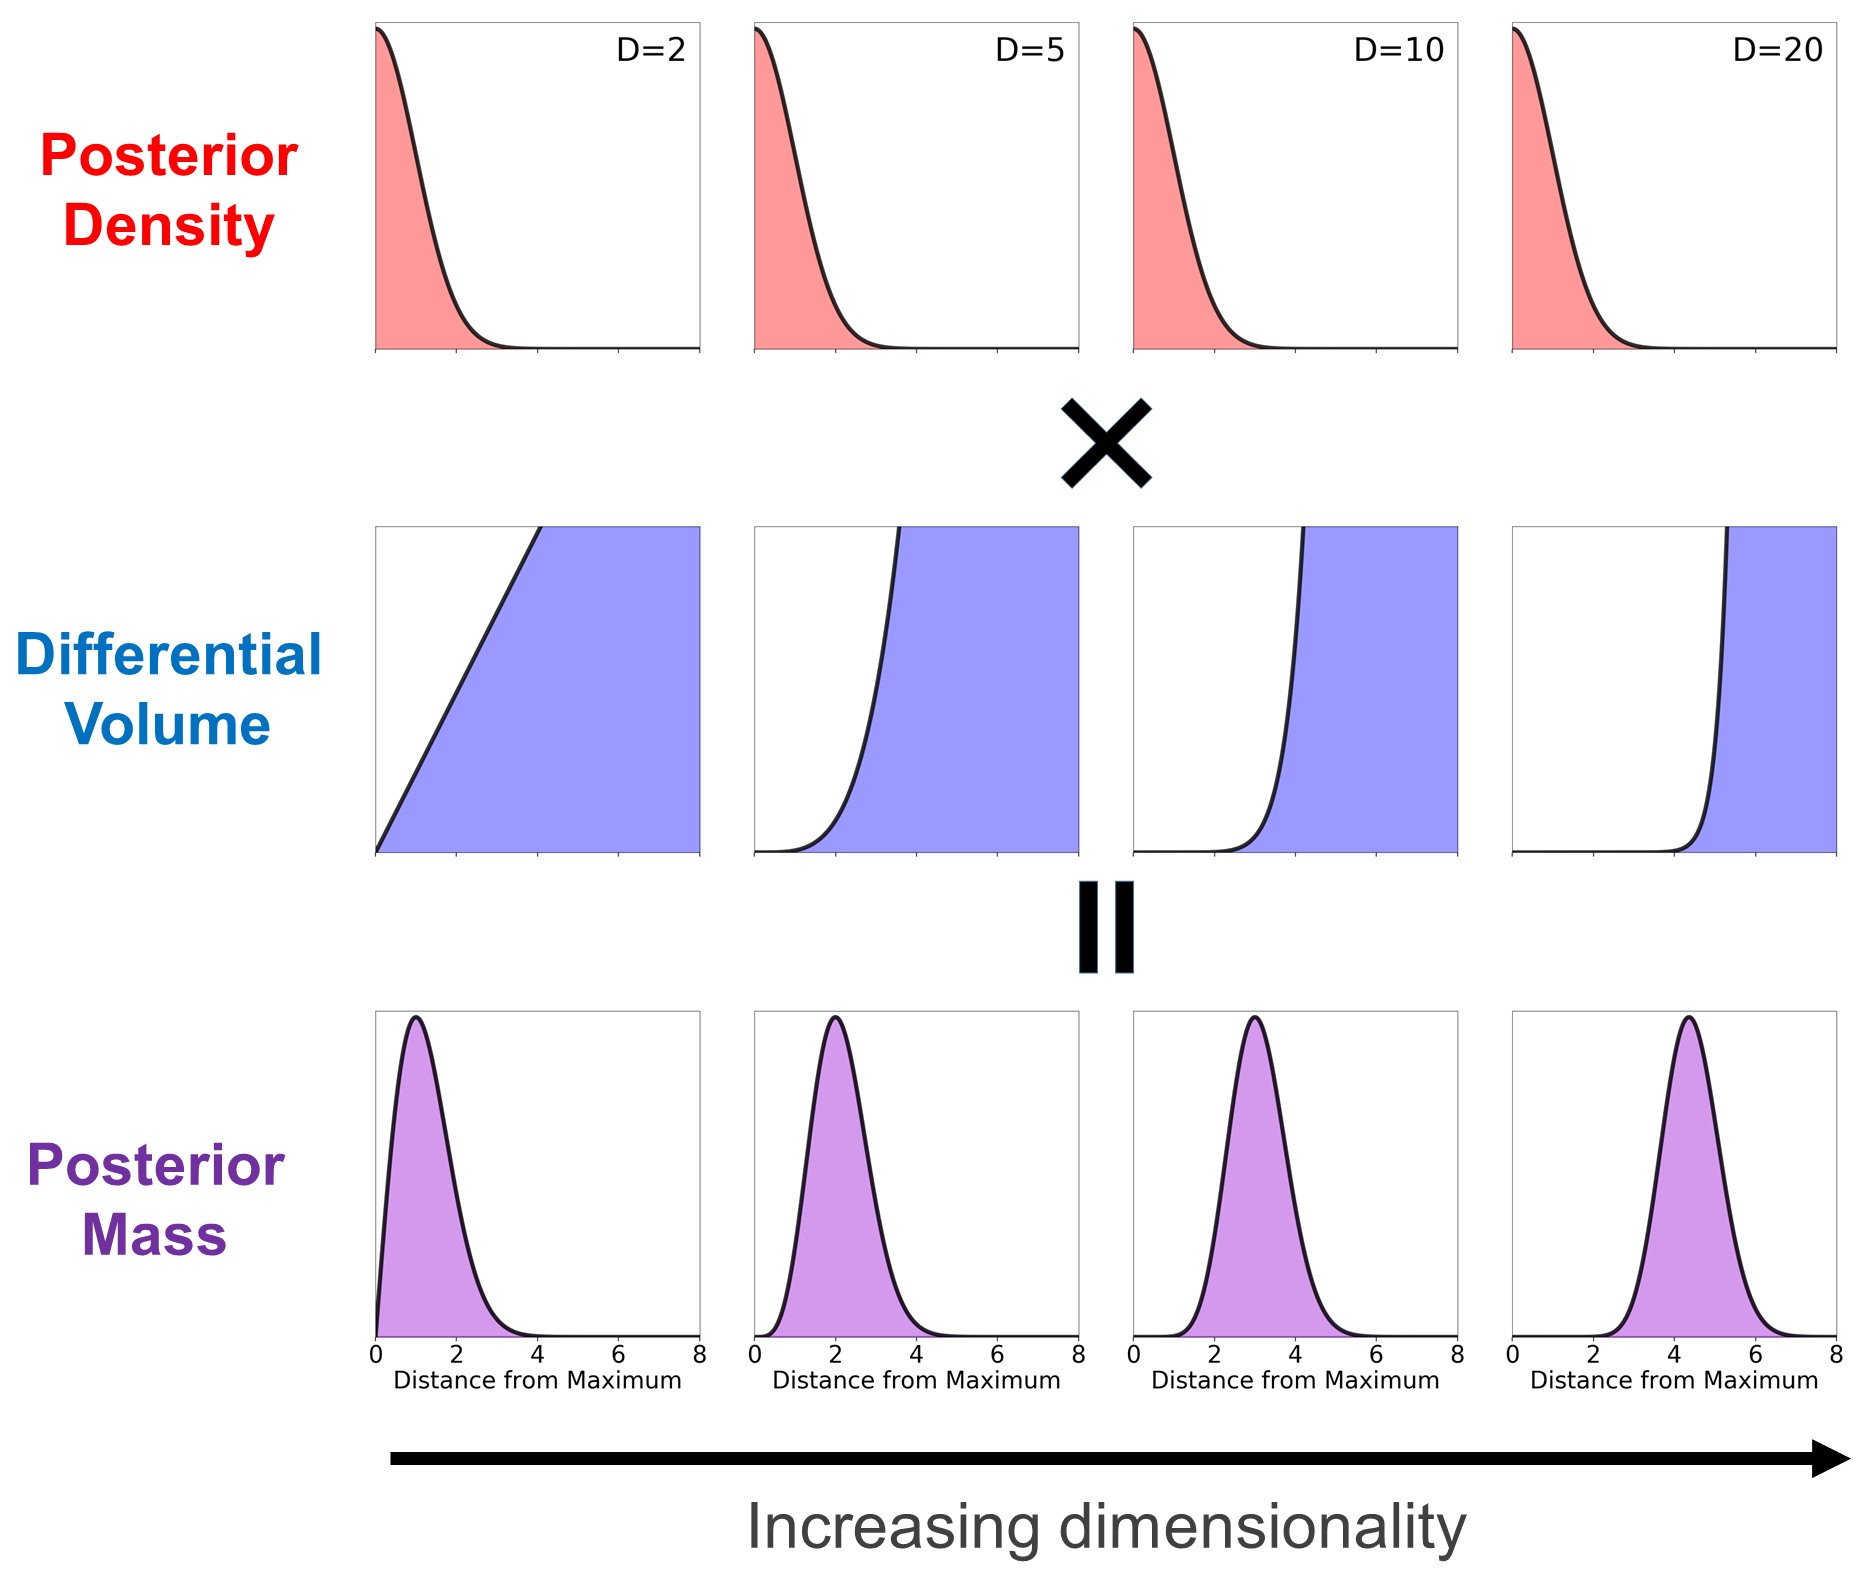
\includegraphics[width=\textwidth]{figures/fig12.png}
\end{center}
\caption{A schematic illustration of how the posterior mass
behaves as a function of dimensionality using a $d$-dimensional
Gaussian. The top panel shows the posterior density 
$\posterior(r) \propto e^{-r^2/2}$ (red) plotted 
as a function of distance $r$ from the maximum posterior density at $r=0$
as the number of dimensions $d$ increases (left to right). As expected,
this distribution remains constant. The middle panel shows
the differential volume element 
$\deriv V(r) \propto r^{d-1} \deriv r$ (blue) of
the corresponding shell at radius $r$. This illustrates the
exponentially increasing volume contributed by shells further
away from the maximum. The bottom panel shows corresponding
``posterior mass'' as a function of radius 
$\posterior'(r) \propto r^{d-1} \posterior(r) \propto r^{d-1} e^{-r^2/2}$ (purple).
Due to the increasing amount of volume located further away from
the maximum posterior density, we see that the majority of the
posterior mass (and therefore of any samples we generate with MCMC)
are actually located a shell located far away from the $r=0$.
See \S\ref{subsec:mass} for additional details.
}\label{fig:mass}
\end{figure}

This result has two immediate implications. First, \textit{the majority
of our samples are not located where the posterior
density is maximized}. This is the result of an exponentially
increasing number of parameter combinations, which allow a
small handful of excellent fits to the data to
be easily overwhelmed by a substantially larger number
of mediocre fits. MCMC methods are therefore generally
inefficient at locating and/or characterizing the region of
peak posterior density.

Second, as $d$ increases we generally would expect the radius of the
shell containing the bulk of the posterior mass to increase, moving further
and further away from the peak density due to the exponentially increasing
available volume. Since the majority of our samples are located in this
region, \textit{our chain will spend the vast majority 
of time generating samples from this shell}.

This allows us to now outline exactly why it is challenging
to propose samples efficiently in high dimensions:
\begin{enumerate}
    \item To make sure our acceptance fractions remain reasonable, 
    we need to ensure our proposed positions mostly lie within 
    this shell of posterior mass.
    \item However, obtaining an independent sample requires 
    being able to (in theory) propose any position within this shell.
    \item This means that our auto-correlation time
    will principally be set by how long it takes to ``wander around''
    the shell, which will be a function of its overall size $r'$,
    its width $\Delta r'$, and the number of dimensions $d$.
\end{enumerate}

\section{Application to a Simple Toy Problem} \label{sec:example}

I now consider a concrete, detailed example
to illustrate how all the concepts discussed in \S\ref{sec:mcmc} and
\S\ref{sec:sampling} come together in practice. 
Throughout this section, I will outline a number of analytic
results and utilize several different MCMC sampling strategies
to generate chains of samples. I strongly encourage interested readers
to implement their own versions of the methods outlined here,
which can be used to reproduce the numerical results from this section
in their entirety.

\subsection{Toy Problem} \label{subsec:analytic}

In this toy problem, we will take our (unnormalized) 
posterior to be a $d$-dimensional 
Gaussian (Normal) distribution with a mean
of $\mu = 0$ and a standard deviation of $\sigma$
in all dimensions:
\begin{equation}
    \tilde{\posterior}(\params) 
    = \exp\left[-\frac{1}{2}\frac{|\params|^2}{\sigma^2}\right]
\end{equation}
where $|\params|^2 = \sum_{i=1}^{d} \Theta_i^2$ is the squared magnitude
of the position vector.

Based on the results from \S\ref{subsec:mass}, 
we can better understand the properties of this distribution by
rewriting the posterior density
in terms of the ``radius''
$r \equiv | \params | = \sqrt{\sum_{i=1}^{d} \Theta_i^2}$
away from the center:
\begin{equation}
    \tilde{\posterior}(r) = \exp\left[-\frac{r^2}{2\sigma^2}\right]
\end{equation}
The corresponding volume contained within a given radius $r$ is then
\begin{equation}
    V(r) \propto r^d
\end{equation}
The corresponding posterior mass is $\tilde{\posterior}'(r)$
is then defined via
\begin{align}
    \tilde{\posterior}(V) \deriv V(r)
    \propto e^{-r^2/2\sigma^2} r^{d-1} \deriv r \nonumber
    \equiv \tilde{\posterior}'(r) \deriv r
\end{align}
Note that this is closely related
to the \textbf{chi-square distribution}.

The \textbf{typical radius} $r_{\rm peak}$ 
where the posterior mass peaks (i.e. is maximized)
and a sample is most likely to be located
can be derived by setting $\deriv \tilde{\posterior}'(r)/\deriv r = 0$.
Solving this gives
\begin{equation}
    r_{\rm peak} = \sqrt{d-1} \sigma
\end{equation}
In other words, while in 1-D a typical sample
is most likely to be located at the peak of the 
distribution with $r_{\rm peak} = 0$, in higher dimensions
this changes quite drastically. While $r_{\rm peak} = 1\sigma$
in 2-D, it is $2\sigma$ in 5-D, $3\sigma$ in 10-D, and $5\sigma$
in 26-D. This is a direct consequence of the
huge amount of volume at larger radii in high dimensions:
although a sample at $r=5\sigma$ has a posterior density $\posterior(r)$
orders of magnitude worse than a sample at $r=0$, the enormous number of
parameter combinations (volume) available at $r=5\sigma$
more than makes up for it.

In general, we expect the posterior mass to comprise
a \textbf{``Gaussian shell''} centered at some radius
\begin{equation}
    r_{\rm mean} \equiv \meanwrt{r}{\posterior'}
    = \int_0^\infty r \posterior'(r) \deriv r
    = \sqrt{2} \frac{\Gamma\left(\frac{d+1}{2}\right)}
    {\Gamma\left(\frac{d}{2}\right)} \sigma
    \approx \sqrt{d} \sigma
\end{equation}
with a standard deviation of
\begin{equation}
    \Delta r_{\rm mean}
    \equiv \sqrt{\meanwrt{(r - r_{\rm mean})^2}{\posterior'}}
    = \sigma \sqrt{d - 2 
    \left(\frac{\Gamma\left(\frac{d+1}{2}\right)}
    {\Gamma\left(\frac{d}{2}\right)}\right)^2}
    \approx \frac{\sigma}{\sqrt{2}}
\end{equation}
where $\Gamma(d)$ is the Gamma function and the
approximations are taken for large $d$.
See {\color{red} \autoref{fig:mass}} for an
illustration of this behavior.

\subsection{MCMC with Gaussian Proposals} \label{subsec:mcmc_gauss}

Let us now consider a chain of samples
$\{ \params_1 \rightarrow \dots \rightarrow \params_n \}$.
The distance between two samples
$\params_m$ and $\params_{m+t}$ 
separated by some lag $t$ will be
\begin{equation}
    |\params - \params'|
    = \sqrt{\sum_{i=1}^{d} (\Theta_{m,i} - \Theta_{m+t,i})^2}
\end{equation}
Assuming that the lag $t \gg \tau$ is
substantially larger than the auto-correlation time $\tau$,
we can assume each sample is approximately iid distributed following
our Gaussian posterior. This then gives an expected separation of
\begin{equation}
    \Delta r_{\rm sep} 
    \equiv \sqrt{\meanwrt{|\params_{m} - \params_{m+t}|^2}{\posterior}}
    = \sqrt{\sum_{i=1}^{d} \meanwrt{(\Theta_{m,i} - \Theta_{m+t,i})^2}{\posterior}}
    = \sqrt{2d} \sigma \approx \sqrt{2} r_{\rm mean}
\end{equation}

We can in theory propose samples in such a way so that the separation
$|\params_{i+1} - \params_{i}|$
between a proposed position $\params_{i+1}$ 
and the current position $\params_i$ follows the
ideal separation of $\sqrt{2}r_{\rm mean}$ derived above
by using a simple Gaussian proposal distribution:
\begin{equation}
    \proposal(\params_{i+1}|\params_i)
    \propto \exp\left[-\frac{1}{2}\frac{|\params_{i+1} - \params_i|^2}{2\sigma^2}\right]
\end{equation}
While this proposal has the same \textit{shape} as the posterior,
it is centered on $\params_i$ rather than $0$. Using our intuition for
how volume behaves based on \S\ref{subsec:volume}, we can
conclude that the majority of samples proposed from 
this choice of $\proposal(\params'|\params)$ will probably have little overlap
with the posterior. 

\begin{figure}
\begin{center}
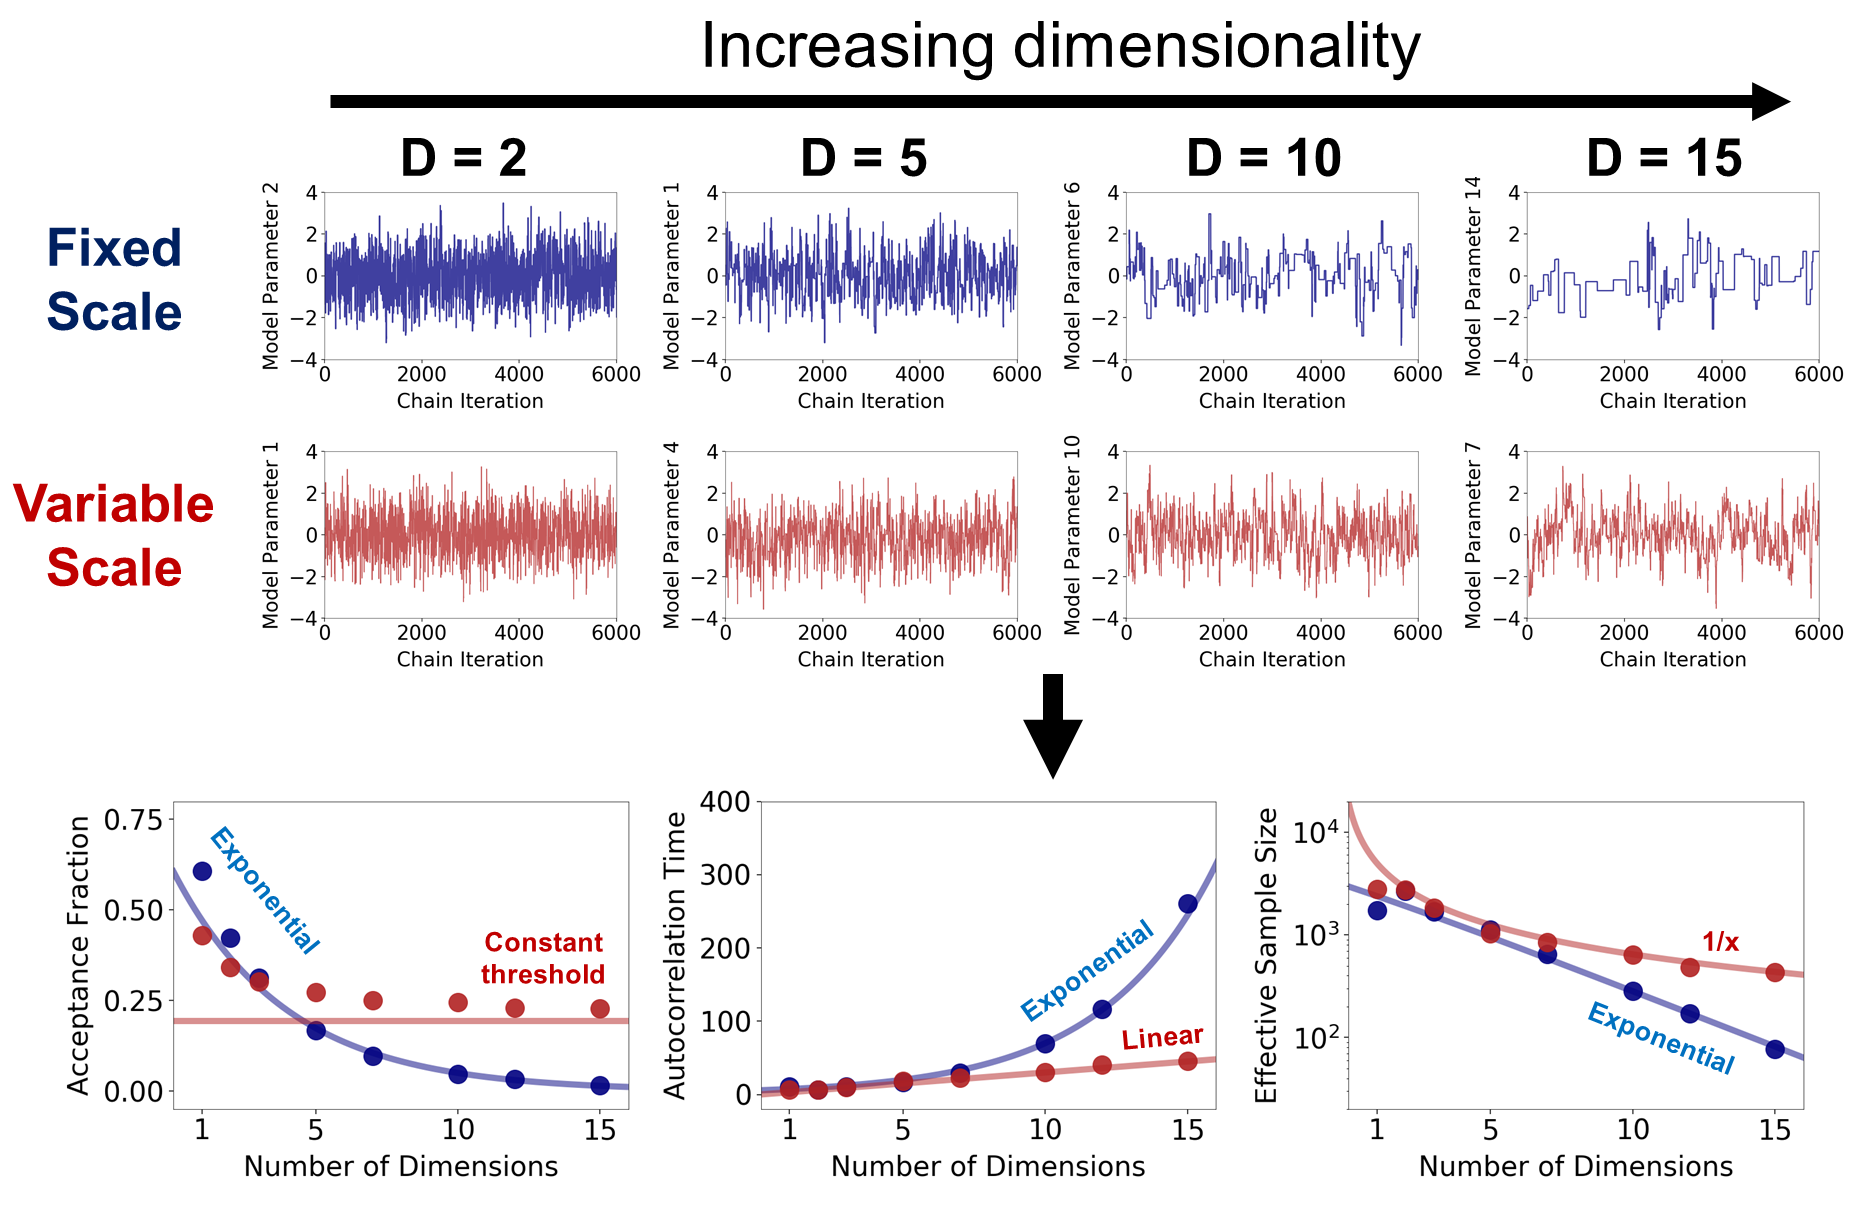
\includegraphics[width=\textwidth]{figures/fig13.png}
\end{center}
\caption{Numerical results showcasing the performance
of a simple MH MCMC sampler with Gaussian proposals
on our toy problem, a $d$-dimensional Gaussian with mean $\mu=0$
and standard deviation $\sigma=1$ in every dimension.
The top series of panels show snapshots of a random parameter
from the chain as a function of dimensionality (increasing
from left to right) assuming an unchanging proposal with
constant scale factor $\gamma=\sqrt{2}$ (blue) 
and a shrinking proposal with $\gamma=2.5/\sqrt{d}$ designed
to target a constant acceptance fraction of $\sim 25\%$ (red).
The bottom panels show the corresponding
acceptance fractions (left), auto-correlation times (middle), and
effective sample sizes (right) from our chains (colored points)
as a function of dimensionality. The approximations from 
\S\ref{subsec:mcmc_gauss} are shown as light colored lines.
Shrinking the size of the proposal helps to keep samples 
within the bulk of the posterior mass, substantially reducing
the auto-correlation time and increasing the effective sample size.
Failing to do so leads to
an exponentially decreasing fraction of good
proposals and a corresponding exponential increase/decrease in the
auto-correlation time/effective sample size.
See \S\ref{subsec:mcmc_gauss} for additional discussion.
}\label{fig:mcmc_gauss}
\end{figure}

Indeed, numerical simulation suggests
the typical fraction of positions that will be accepted given the above proposal
roughly scales as
\begin{equation}
    \langle f_{\rm acc}(d) \rangle
    \equiv \exp\left[\meanwrt{\ln T(\params_{i+1}|\params_i)}
    {\posterior,\proposal}\right]
    \sim \exp\left[-\frac{d}{4} - \frac{1}{2}\right]
\end{equation}
which decreases exponentially as the dimensionality increases,
similar to {\color{red} \autoref{fig:vol}}. Likewise, we find
the auto-correlation time roughly scales as
\begin{equation}
    \langle \tau(d) \rangle 
    \equiv \exp\left[\meanwrt{\ln \tau}
    {\posterior,\proposal}\right]
    \sim \exp\left[\frac{d}{4} + \frac{7}{4}\right]
\end{equation}
This exponential dependence
arises because the overlap between the typical Gaussian proposal
$\proposal(\params'|\params)$ and the underlying posterior 
$\posterior(\params)$ essentially reduces to the small volume
where two thin shells overlap. Since the radii of the shells
goes as $\propto \sqrt{d}$ while the widths remain roughly constant,
the ``fractional size'' of the shell (and the corresponding overlap)
ends up decreasing exponentially.

To counteract this effect, we need to adjust the $\sigma$ of our
proposal distribution by some factor $\gamma$:
\begin{equation}
    \proposal_\gamma(\params_{i+1}|\params_i)
    \propto \exp\left[-\frac{1}{2}\frac{|\params_{i+1} - \params_i|^2}
    {(\gamma\sigma)^2}\right]
\end{equation}
where our previous proposal assumes $\gamma = \sqrt{2}$.
If we want to ensure our typical acceptance fraction will remain
roughly constant as a function of dimension $d$, $\gamma$ needs to scale as
\begin{equation}
    \langle f_{\rm acc}(\gamma(d)) \rangle \approx C
    \quad \Rightarrow \quad
    \gamma(d) \propto \frac{1}{\sqrt{d}}
\end{equation}
which inversely tracks the expected radius $r_{\rm mean}$
of the typical set. We find that taking
\begin{equation}
    \gamma = \frac{\delta}{\sqrt{d}}
\end{equation}
leads to a typical acceptance fraction of
\begin{equation}
    \langle f_{\rm acc}(\delta/\sqrt{d}) \rangle
    \approx \exp\left[-\left(\frac{\delta^2}{4}\right)^{2} 
    - \frac{\delta}{2}\right]
\end{equation}
as $d$ becomes large with a typical auto-correlation time of
\begin{equation}
    \langle \tau(\delta/\sqrt{d}) \rangle \approx 3 d
\end{equation}
for reasonable choices of $\delta$.
This linear dependence is a substantial improvement over
our earlier exponential scaling.

\subsubsection*{Numerical Tests} \label{subsubsec:sims_1}

To confirm these results, I sample from this $d$-dimensional
Gaussian posterior (assuming $\sigma=1$ for simplicity) using
two MH MCMC algorithms for $n=20,000$ iterations
based on these proposal distributions.
The first proposes new points 
assuming $\gamma=\sqrt{2}$. The second
assumes $\gamma=2.5/\sqrt{d}$ in order
to maintain a roughly constant acceptance fraction of 25\%. 
As shown in {\color{red} \autoref{fig:mcmc_gauss}}, the chains
behave as expected given our theoretical predictions as a function
of dimensionality, with the constant proposal quickly becoming stuck
while the adaptive proposal continues sampling normally. While
the auto-correlation time $\tau$ increases in both cases, 
the increase in the latter case (where it is driven by decreasing
size/scale of the proposal distribution)
is much more manageable than the former (where it is driven by
the exponentially decreasing acceptance fraction).

\subsection{MCMC with Ensemble Proposals} \label{subsec:mcmc_ensemble}

One drawback to the Gaussian proposals explored above is that
we have to specify the structure of the distribution ahead of time.
In this specific case, we assumed that:
\begin{enumerate}
    \item the width of the posterior in each dimension (parameter)
    was constant such that $\sigma_1 = \sigma_2 = \dots = \sigma_n = \sigma$ and
    \item the parameters were entirely uncorrelated with each other such that
    the correlation coefficient $\rho_{ij} = 0$ between any two dimensions
    $i$ and $j$.
\end{enumerate}

In general, there is no good reason to assume that either of these are true.
This means we have to also estimate the entire set of
$d(d+1)/2$ free parameters that determine the overall covariance
structure of our unknown posterior distribution.
Trying to adjust the covariance structure in order
to improve our sampling efficiency and decrease the auto-correlation
time (see \S\ref{exercise:importance} and \S\ref{exercise:mcmc})
becomes one of the most difficult parts of running MCMC algorithms in practice.

While there are schemes to perform these adjustments during
an extended burn-in period (see, e.g., \citealt{brooks+11}), there
is significant appeal in methods that can ``auto-tune'' without
much additional input from the user. One class of such approaches
are known as \textbf{ensemble} or \textbf{particle} methods.
These methods attempt to use many $m$ chains running
simultaneously (i.e. in parallel) to improve the performance 
of any individual chain.

We explore three variations of ensemble methods here
that attempt to exploit $m \gtrsim d(d+1)/2$ chains running
simultaneously:
\begin{enumerate}
    \item using the ensemble of particles to condition
    a Gaussian proposal distribution,
    \item using trajectories from multiple particles along with
    Gaussian ``jitter'', and
    \item using affine-invariant transformations of
    trajectories from multiple particles.
\end{enumerate}
A schematic illustration of these 
methods is shown in {\color{red} \autoref{fig:mcmc_particles}}.

As we might expect, an immediate drawback of these methods is
they rely on having enough particles to characterize
the overall structure of the space (i.e. the curse of dimensionality).
While this limits their utility when sampling from high-dimensional spaces, 
they can be attractive options in moderate-dimensional spaces 
($d \lesssim 25$) where a few hundred particles
are often sufficient to ensure reasonable performance.

\begin{figure}
\begin{center}
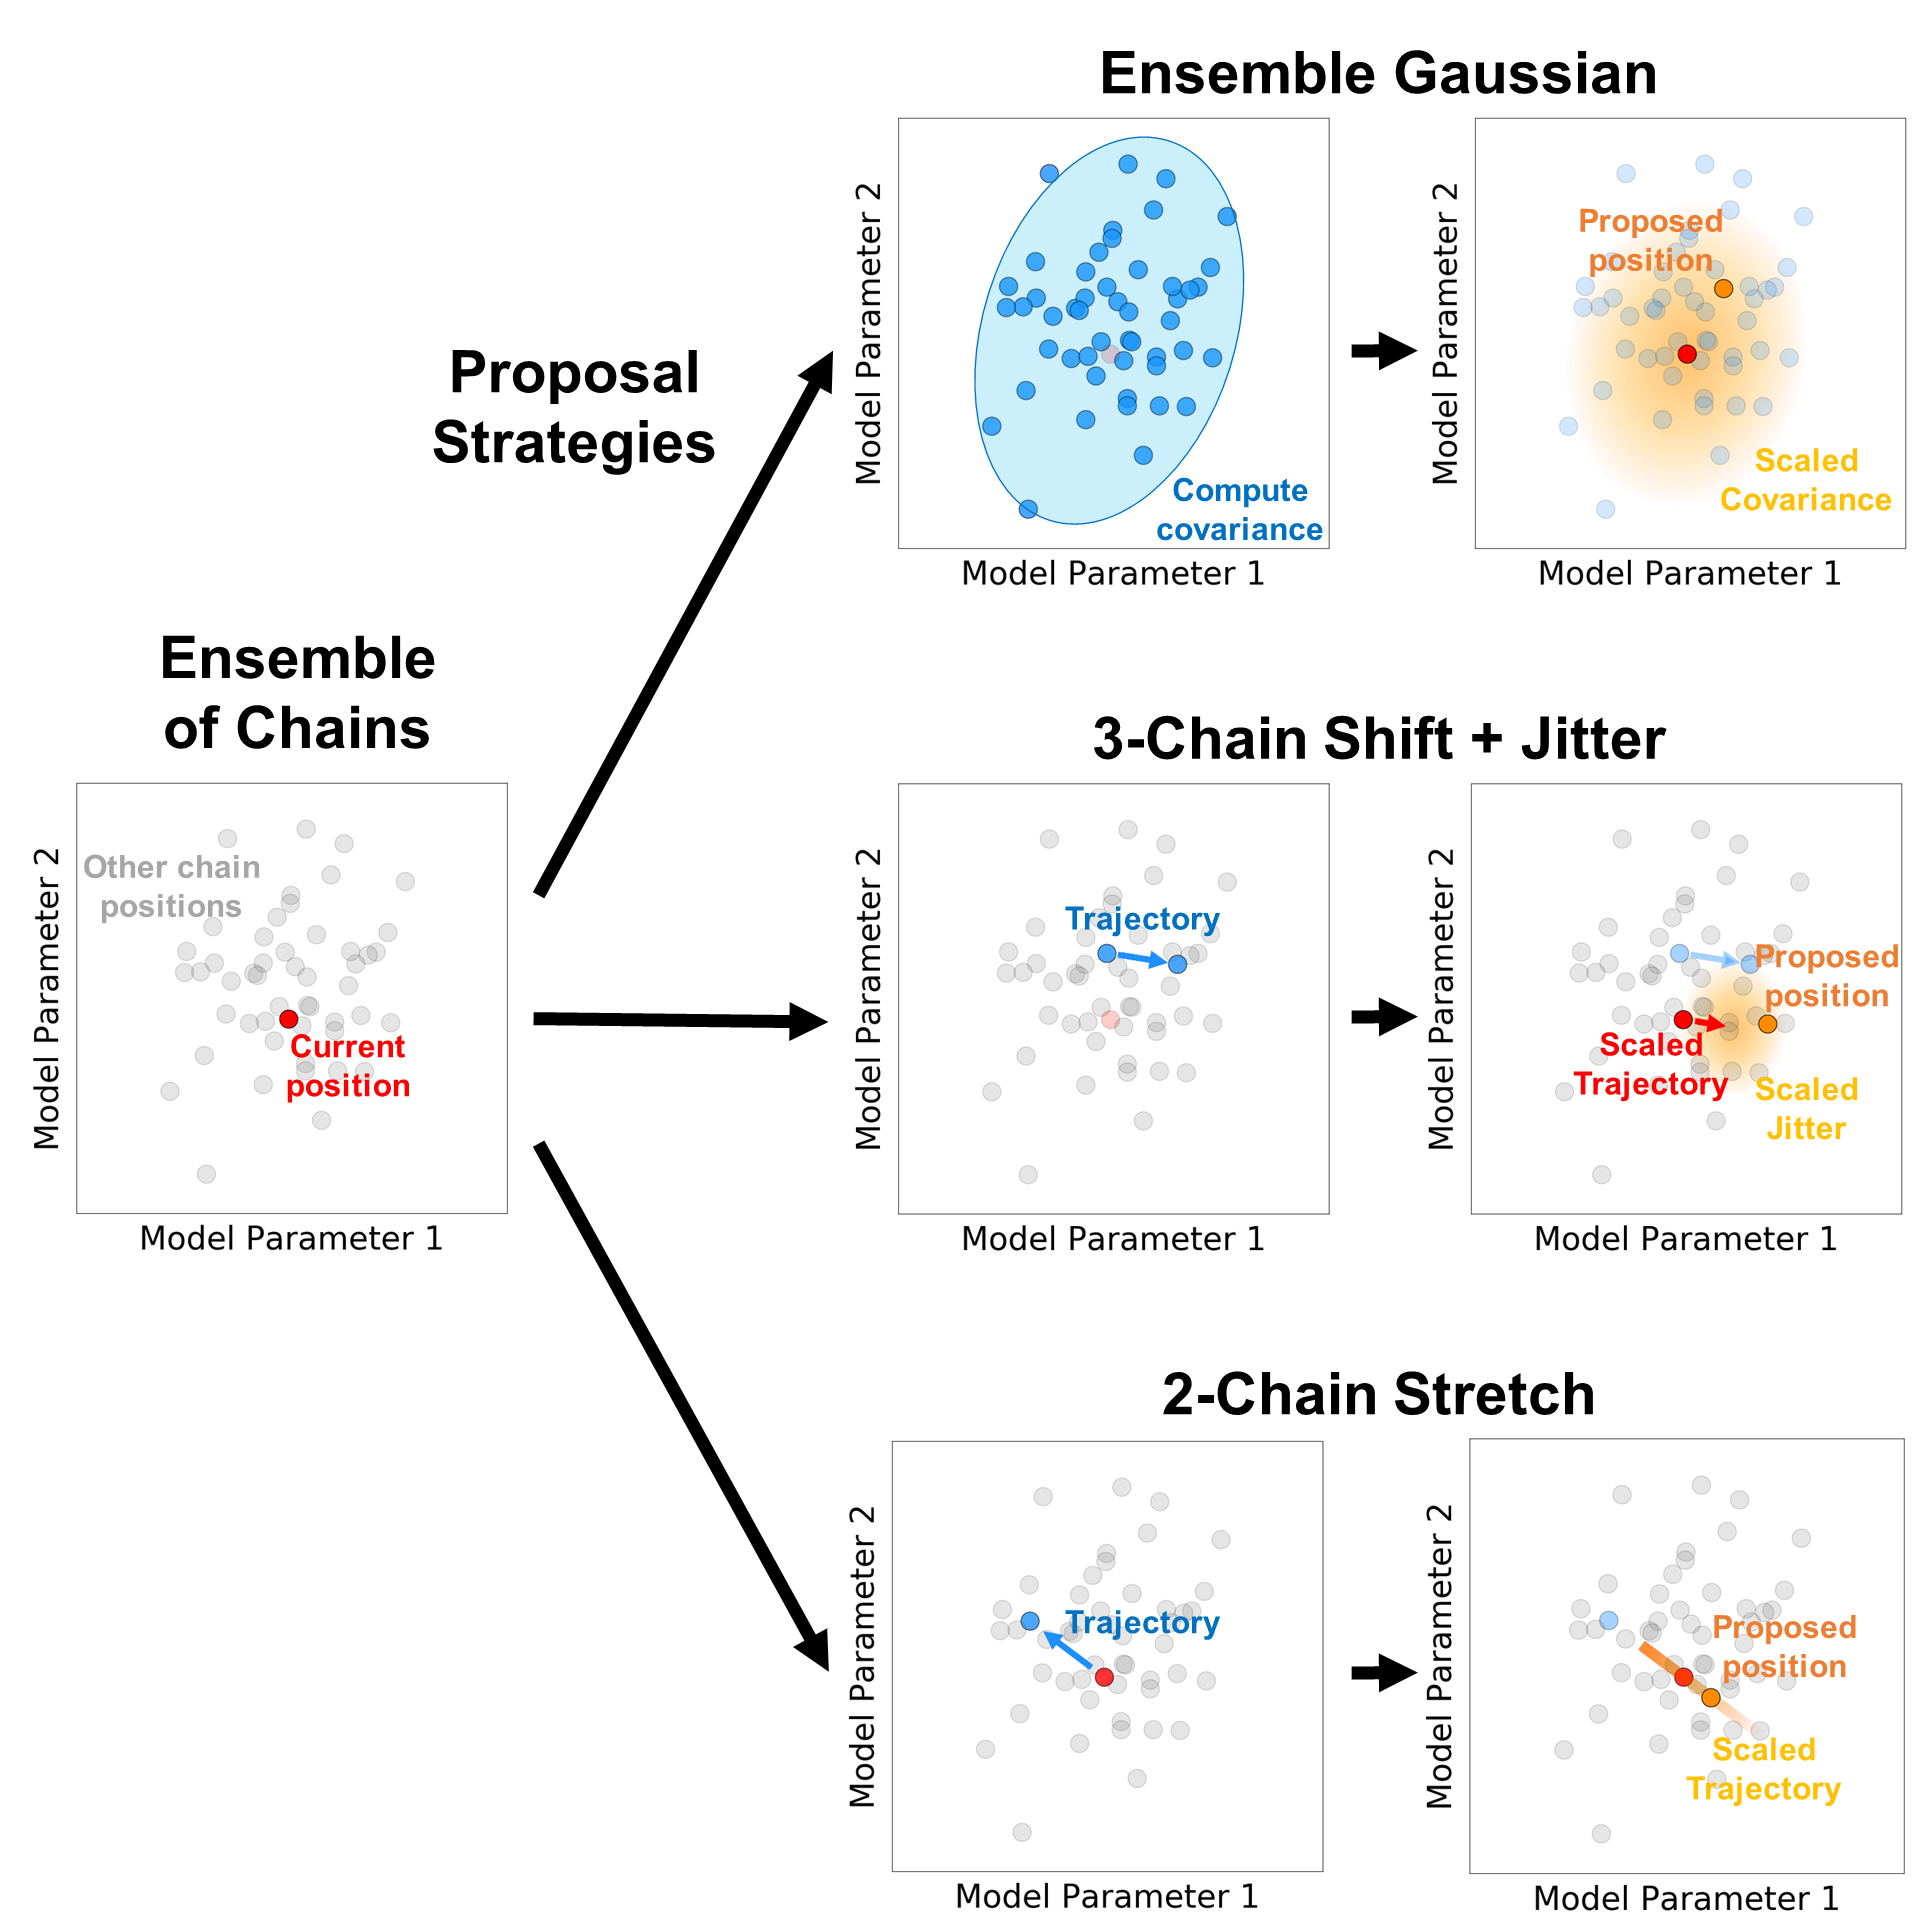
\includegraphics[width=\textwidth]{figures/fig14.png}
\end{center}
\caption{A schematic illustration of the three ensemble MCMC
methods described in \S\ref{subsec:mcmc_ensemble}. 
The current state of the chain we are interested in updating (red)
and the other chains in the ensemble (gray) are shown on the left.
In the top panels (ensemble Gaussian; \S\ref{subsubsec:ensemble_gauss}),
we compute the covariance of the other $k \neq j$
chains (middle) and use a scaled version to subsequently
propose a new position. 
In the middle panels (3-chain shift + jitter; \S\ref{subsubsec:demcmc}),
we use two additional chains $k \neq l \neq j$ to compute a trajectory. 
We then propose a new position based on this scaled trajectory plus
a small amount of ``jitter''. 
In the bottom panels (2-chain stretch; \S\ref{subsubsec:emcee}), we use
only one additional chain $k \neq j$ to propose a new trajectory. We
then propose a random position along a scaled version of this
trajectory with the proposal probability 
varying as a function of scale.
See \S\ref{subsec:mcmc_ensemble} for additional details.
}\label{fig:mcmc_particles}
\end{figure}

\subsubsection{Gaussian Proposal} \label{subsubsec:ensemble_gauss}

The first approach is simply a modified
Gaussian proposal: at any iteration $i$ for any chain
$j$, we propose a new position $\params_{i+1}^{j}$
based on the current position $\params_{i}^{j}$
using a Gaussian proposal
\begin{equation}
    \proposal_\gamma^j(\params_{i+1}^{j}|\params_{i}^j)
    \propto \exp\left[-\frac{1}{2}
    (\params_{i+1}^{j} - \params_{i}^{j})^{\rm T}
    (\gamma^2\cov_i^j)^{-1}
    (\params_{i+1}^{j} - \params_{i}^{j})\right]
\end{equation}
where ${\rm T}$ is the transpose operator and
\begin{equation}
    \cov_i^j = {\rm Cov}\left[\{\params_i^1, \dots, 
    \params_i^{j-1}, \params_i^{j+1}, \dots, \params_i^m\}\right]
\end{equation}
is the empirical covariance matrix estimated from the
current positions of the $m$ chains \textit{excluding} chain $j$.
We repeat this process for each of the $m$ chains in turn.

In other words, at each iteration $i$ we want to update all
$m$ chains. We do so by updating each chain $j$ in turn based on what
the other chains are currently doing. Assuming the current position of
each chain is distributed following the underlying posterior
$\posterior(\params)$, it is straightforward to show that
$\cov_i^j$ is a reasonable approximation to the unknown
covariance structure of our posterior. In addition,
because we exclude $j$ when computing $\cov_i^j$, this proposal
is symmetric going from $\params_{i}^{j} \rightarrow \params_{i+1}^{j}$
and from $\params_{i+1}^{j} \rightarrow \params_{i}^{j}$.
This means that we satisfy detailed balance and do not
have to incorporate any proposal-dependent factors when
computing the transition probability.

\subsubsection{Ensemble Trajectories with a Gaussian Proposal} 
\label{subsubsec:demcmc}

The approach taken in \S\ref{subsubsec:ensemble_gauss}
solves the problem of trying to tune
the covariance of our initial Gaussian proposal. However, it still
assumes that a Gaussian proposal is the optimal solution.
A more general approach is one that does not rely on assuming a
proposal explicitly, but rather only relies on the distribution of
the remaining particles. 

One such approach used in the literature is
\textbf{Differential Evolution} MCMC \citep[DE-MCMC;][]{stornprice97,terbraak06}.
The main idea behind DE-MCMC is to rely on the \textit{relative positions}
of the chains at a given iteration $i$ when making new proposals. We first
randomly select two other particles $k$ and $l$ where
$\params^j_i \neq \params^k_i \neq \params^l_i$. We then propose
a new position based on the vector distance between the other
two particles $\params^k_i - \params^l_i$ with some scaling $\gamma$
along with some additional ``jitter'' $\epsilon$:
\begin{equation}
    \params_{i+1}^{j} 
    = \params_i^j + \gamma \times (\params^{k}_i - \params^l_i + \epsilon)
\end{equation}

In the case where the behavior of chains $k$ and $l$ are approximately
independent of each other and assuming the
underlying posterior distribution $\posterior(\params)$
is Gaussian with some unknown
mean $\meanvec$ and covariance $\cov$
(and ``standard deviation'' $\cov^{1/2}$), it is straightforward to
show that the distribution of $\params^k_i - \params^l_i$ will then follow
\begin{equation}
    \params^k_i - \params_l \sim \Normal{\mathbf{0}}{(2\cov)^{1/2}}
\end{equation}
Typically, the jitter $\epsilon$ is chosen to also be Gaussian distributed
with covariance $\cov_\epsilon$ such that
\begin{equation}
    \epsilon \sim \Normal{\mathbf{0}}{\cov_\epsilon^{1/2}}
\end{equation}
In general, $\cov_\epsilon$ is mostly
used to try and avoid issues caused by finite particle
sampling: since the number of unique trajectories (ignoring symmetry) is
\begin{equation*}
    n_{\rm traj} 
    = \binom{m-1}{2} 
    = \frac{(m-1)!}{2!(m-3)!}
    = \frac{(m-1)(m-2)}{2}
\end{equation*}
if $m$ is sufficiently small the DE-MCMC
procedure can only explore a small number of possible trajectories
at any given time, leading to extremely inefficient sampling.

Combined, this implies that the
proposed position has a distribution of
\begin{equation}
    \params_{i+1}^{j} 
    \sim \Normal{\params_i^j}{\gamma \times (2\cov+\cov_\epsilon)^{1/2}}
\end{equation}
This shows that the 3-particle DE-MCMC procedure can generate
new positions in a manner analogous to the ensemble Gaussian proposal
we first discussed.

\subsubsection{Affine-Invariant Transformations of Ensemble Trajectories}
\label{subsubsec:emcee}

Another approach used in the literature 
\citep[e.g., {\texttt{emcee}};][]{foremanmackey+13_alt}
is the \textbf{Affine-Invariant ``stretch move''} from 
\citet{goodmanweare10}. This 
uses only one additional particle $\params_i^k$ rather than two:
\begin{equation}
    \params_{i+1}^{j} 
    = \params_i^k + \gamma \times (\params^{j}_i - \params^k_i)
\end{equation}
In place of the jitter term $\epsilon$ from DE-MCMC,
the stretch move instead injects some amount of 
randomness by allowing $\gamma$ to vary.
By sampling $\gamma$ from some probabilty distribution 
$g(\gamma)$, we allow the proposals
to explore various ``stretches'' of the direction vector.
As shown in \citet{goodmanweare10}, if this function is chosen such that
\begin{equation}
    g(\gamma^{-1}) = \gamma \times g(\gamma)
\end{equation}
then this proposal is symmetric. Typically, $g(\gamma)$ is chosen
to be
\begin{equation}
    g(\gamma|a) = 
    \begin{cases}
    \gamma^{-1/2} & a^{-1} \leq \gamma \leq a \\
    0 & {\rm otherwise}
    \end{cases}
\end{equation}
where $a=2$ is often taken as a typical value.
Note that when $\gamma = 1$, this move leaves 
$\params_{i+1}^j = \params_i^j$ unchanged.

Compared to DEMCMC, the stretch move appears to have one clear advantage:
it doesn't have any reliance on some ``jitter'' term $\epsilon$ that reintroduces
scale-dependence into the proposal. That makes the proposal invariant to
affine transformations and only
sensitive to \textit{a single parameter} $a$, which governs the range of
scales the stretch factor $\gamma$ is allowed to explore.

This lack of jitter, however, is not substantially advantageous in practice. 
As noted in \S\ref{subsubsec:demcmc},
$\epsilon$ is really designed to avoid possible
degeneracies due to the limited number of available trajectories. In that
case we had $(m-1)(m-2)/2 \sim m^2/2$ possible trajectories; here, however, we only
have $m$ (since $\params^j_i$ is always included). This is a \textit{much}
smaller number of possible trajectories at a given $m$, 
making this particular proposal more susceptible to that particular effect.

\begin{figure}
\begin{center}
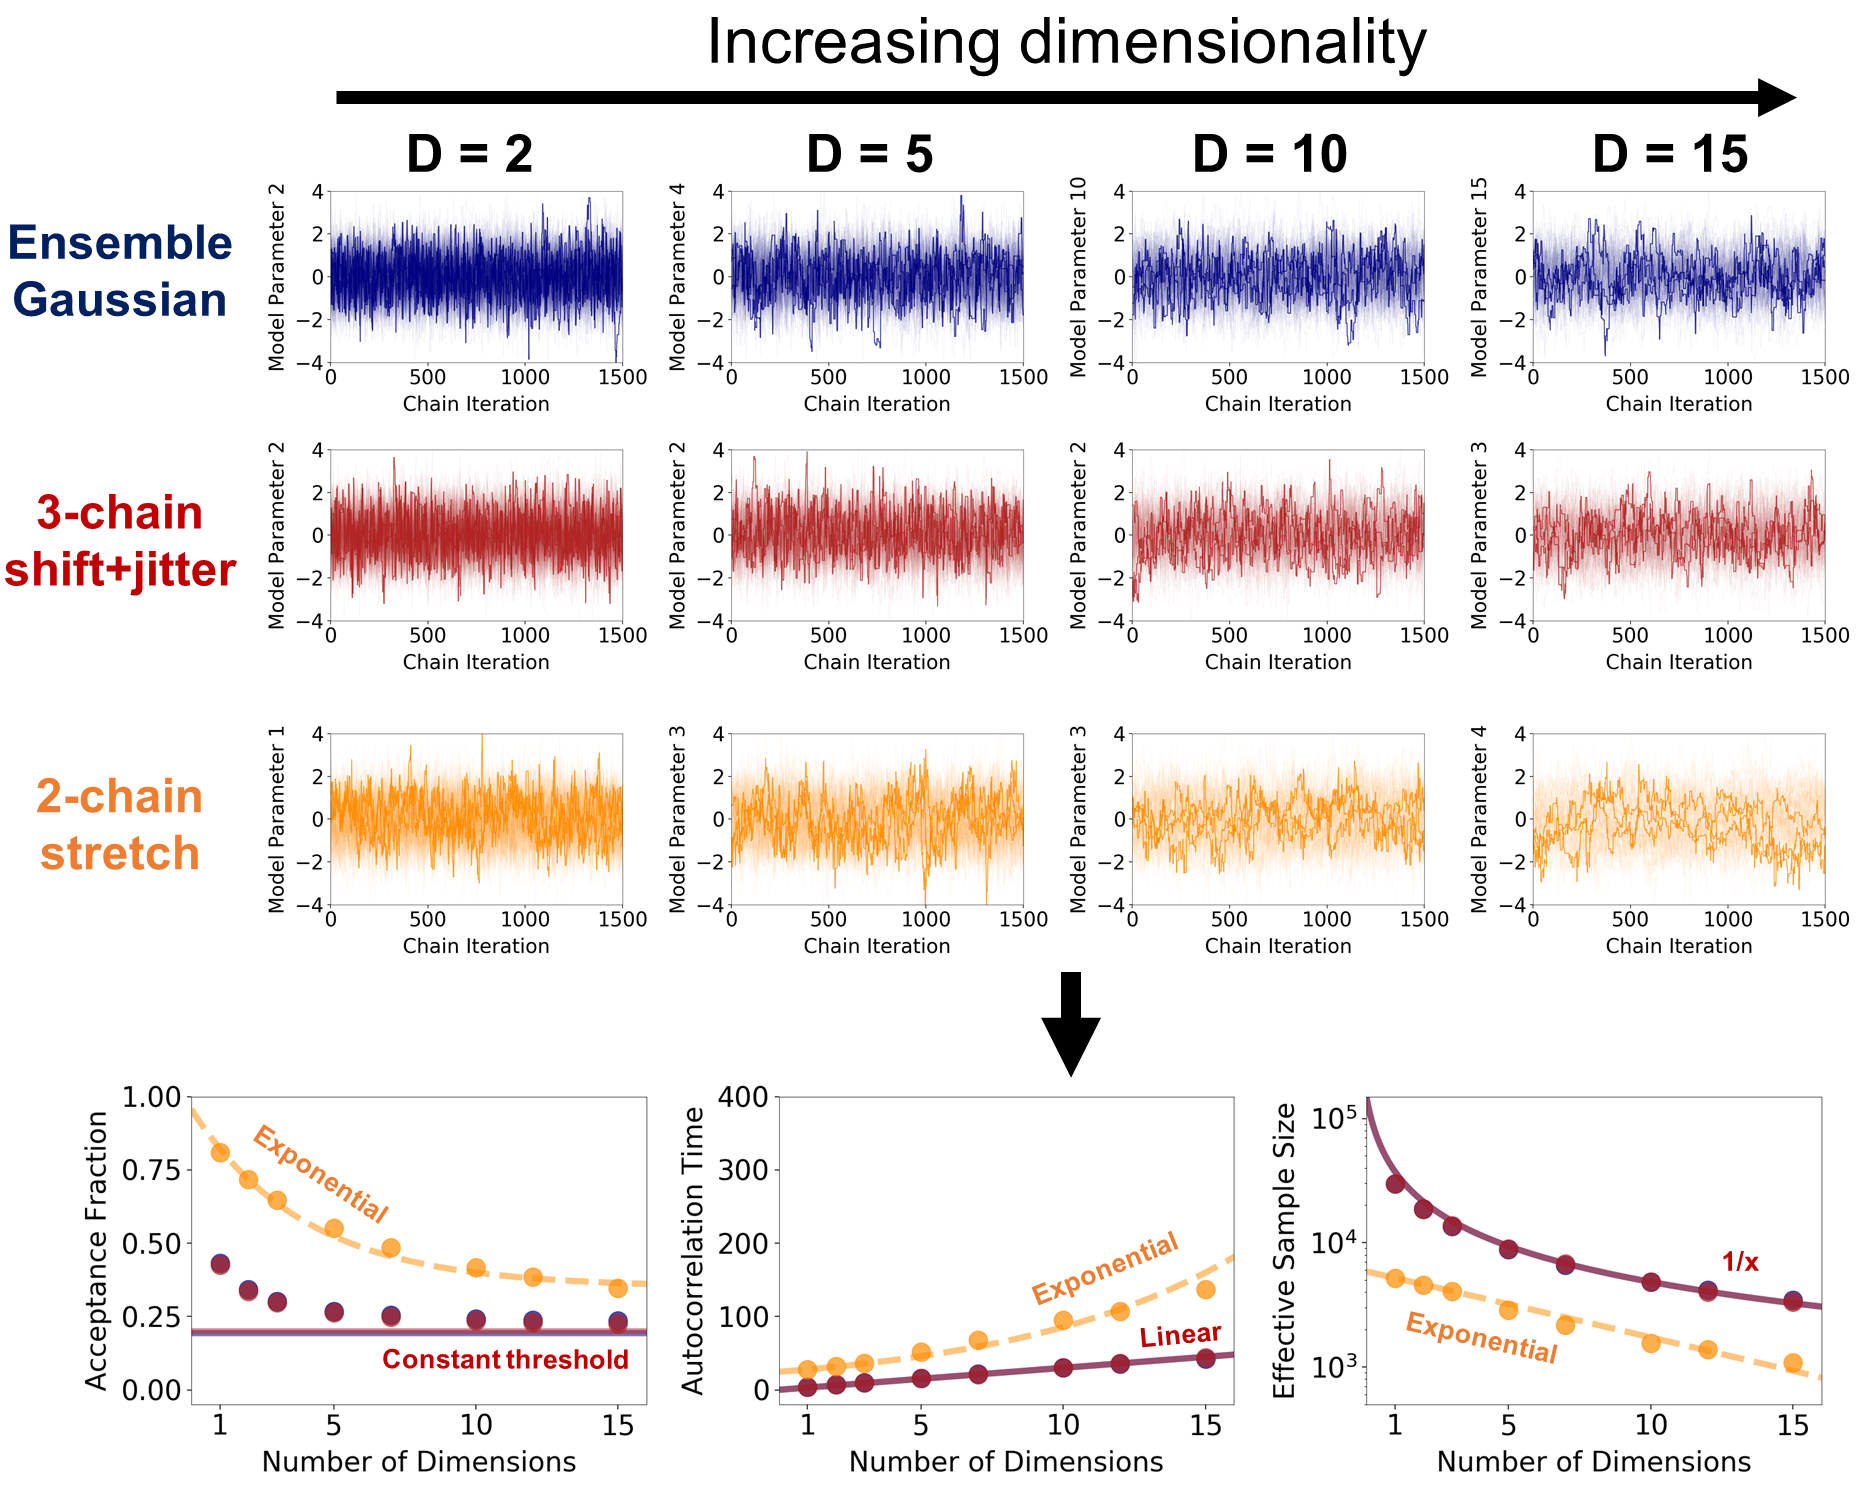
\includegraphics[width=\textwidth]{figures/fig15.png}
\end{center}
\caption{Numerical results showcasing the performance
of several ensemble MH MCMC samplers on our toy problem,
a $d$-dimensional Gaussian with mean $\mu=0$
and standard deviation $\sigma=1$ in every dimension.
The top series of panels show snapshots of a random parameter
from the collection of chains (with a few chains highlighted)
as a function of dimensionality (increasing
from left to right) assuming ensemle Gaussian
proposals with $\gamma=2.5/\sqrt{d}$ (blue), 
3-chain ``shift and jitter''
proposals with $\gamma=1.7/\sqrt{d}$ (red), 
and 2-chain ``stretch'' proposals with
$\gamma$ drawn from the distribution $g(\gamma|a)$ with $a=2$
as described in \S\ref{subsubsec:emcee} (orange).
The bottom panels show the corresponding
acceptance fractions (left), auto-correlation times (middle), and
effective sample sizes (right) from our chains (colored points)
as a function of dimensionality. Approximations based on the 
\S\ref{subsec:mcmc_gauss} are shown as light solid colored lines,
with dashed lines showing rough fits.
The first two methods, which allow the
size of the proposal to shrink, are able to propose samples 
within the bulk of the posterior mass.
The last method, which is unable to do so,
instead proposes exponentially fewer good positions as the
dimensionality increases.
See \S\ref{subsec:mcmc_ensemble} for additional details.
}\label{fig:mcmc_ensemble}
\end{figure}

In addition, because this proposal involves adjusting $\gamma$ and therefore
the length of the trajectory itself, we need to consider how changing $\gamma$
affects the total \textit{volume} of the sphere centered on $\params^j_i$
with radius $\params^k_i-\params^j_i$. As discussed in \S\ref{subsec:volume},
the differential volume increases as $r^{d-1}$. Therefore, increasing
or decreasing $\gamma$ substantially adjusts the differential volume
in our proposal. This involves introducing a steep boost/penalty into our
transition probability, which now becomes:
\begin{equation}
    T(\params_{i+1}^{j}|\params_i^j, \gamma)
    = \min\left[1, \gamma^{d-1} 
    \frac{\posterior(\params^j_{i+1})}{\posterior(\params_i^j)}\right]
\end{equation}
This heavily favors proposals with $\gamma > 1$ (outwards) and heavily
disfavors proposals with $\gamma < 1$ as $d$ increases to account for the
exponentially increasing volume at larger radii.

Finally, while this stretch move actually generates proposals 
in the right overall \textit{direction}, it is not efficient at generating
samples within the bulk of the posterior mass
as the dimensionality increases.
As discussed in \S\ref{subsec:mcmc_gauss}, given the typical
position of $\params_i^j$, the typical length-scale of
the proposed positions needs to shrink by
$\propto 1/\sqrt{d}$ in order to guarantee our new sample
remains within the bulk of the posterior mass.
However, the form for $g(\gamma|a)$ specified above 
instead ensures that $\gamma$ will always be between $1/a$ and $a$.
Even if we attempt to account for this effect by letting 
$a(d) \rightarrow 1$ as $d \rightarrow \infty$ in order to
target a constant acceptance fraction and ensure more overlap, 
the asymmetry of our proposal and the $\gamma^{d-1}$ term
in the transition probability systematically biases our
proposed and accepted positions compared with the ideal distribution.
This subsequently leads to lager auto-correlation times, mostly
counteracting any expected gains.

\subsubsection*{Numerical Tests} \label{subsubsec:sims_2}

To confirm these results, I sample from this $d$-dimensional
Gaussian posterior (assuming $\sigma=1$ for simplicity) 
using each of these ensemble MH MCMC algorithms with for $n=1500$
iterations with $m=100$ chains.
In the first case, I propose a new position for chain $j$ 
at iteration $i$ using a Gaussian distribution with
a covariance $\gamma^2 \cov_i^j$ computed over the remaining ensemble of
$k \neq j$ chains, where the scale factor $\gamma=2.5/\sqrt{d}$ is
chosen to target a constant acceptance fraction of roughly 25\%. 
In the second case, I propose new positions using the DE-MCMC algorithm
with a scale factor of $\gamma=1.7/\sqrt{d}$ 
and additional Gaussian jitter with covariance $\cov_\epsilon = \cov_i^j / 5$
derived from the remaining chains in the ensemble, again targeting
an acceptance fraction of roughly 25\%.
In the third case, I propose new positions using the affine-invariant stretch
move assuming the typical form for $g(\gamma|a)$ with $a=2$.\footnote{Allowing
$a(d)$ to vary as a function of dimensionality to target a roughly constant
acceptance fraction gives similar results.}

As shown in {\color{red} \autoref{fig:mcmc_ensemble}}, the chains
behave as expected given our theoretical predictions as a function
of dimensionality. Similar to the adaptive Gaussian case,
the first two approaches continue 
sampling efficiently even as $d$ increases. The affine-invariant
stretch move, however, experiences exponentially-decreasing efficiency
and struggles to sample the posterior effectively.

\subsection{Additional Comments} \label{subsec:comments}

Before concluding, I wish to emphasize that the toy problem explored in this
section should only be interpreted as a \textit{tool} to build intuition surrounding
how certain methods are expected to behave in a controlled environment.
While the behavior as a function of dimensionality
helps to illustrate common issues, in practice 
the performance of any method will depend on the specific problem, tuning parameters,
the time spent on tuning, and many other possible factors. Since it is always possible
to find problems for which any particular method
will perform well or poorly, I encourage users to try out a variety of
approaches to find the ones that work best for their problems.

\section{Conclusion} \label{sec:conc}

Bayesian statistical methods have become increasingly prevalent in
modern scientific analysis as models have become more complex.
Exploring the inferences we can draw from these models often
requires the use of numerical techniques, the most popular of
which is known as \textbf{Markov Chain Monte Carlo (MCMC)}.

In this article, I provide a conceptual introduction
to MCMC that seeks to highlight the \textit{what}, \textit{why},
and \textit{how} of the overall approach. I first give
an overview of Bayesian inference and discuss \textit{what}
types of problems Bayesian inference generally is trying to solve, 
showing that most quantities we are interested in computing
require integrating over the posterior density.
I then outline approaches to computing these integrals using
grid-based approaches, and illustrate how adaptively changing
the resolution of the grid naturally transitions into 
the use of Monte Carlo methods. I illustrate how
different sampling strategies affect the overall efficiency
in order to motivate \textit{why} we use MCMC methods.
I then discuss various details related to \textit{how} MCMC methods 
work and examine their expected overall behavior based on
simple arguments derived from how volume and posterior density behave
as the number of parameters increases. 
Finally, I highlight the impact this conceptual understanding
has in practice by comparing the performance of various MCMC methods 
on a simple toy problem.

I hope that the material in this article, 
along with the exercises and applications,
serve as a useful resource that helps
build up intuition for how MCMC and other
Monte Carlo methods work.
This intuition should be helpful
when making decisions over when to apply MCMC methods to your own
problems over possible alternatives,
developing novel proposals and sampling strategies, 
and characterizing what issues you might
expect to encounter when doing so.

\section*{Acknowledgements}

JSS is grateful to Rebecca Bleich for continuing to tolerate his
(over-)enthusiasm for sampling during their time together. 
He would also like to thank a number of people for
helping to provide much-needed feedback during earlier stages
of this work, including Catherine Zucker, Dom Pesce, Greg Green,
Kaisey Mandel, Joel Leja, David Hogg, Theron Carmichael, and Jane Huang.
He would also like to thank Ana Bonaca, Charlie Conroy, Ben Cook,
Daniel Eisenstein, Doug Finkbeiner, Boryana Hadzhiyska, 
Will Handley, Locke Patton, and Ioana Zelko
for helpful conversations surrounding the material.

JSS also wishes to thank Kaisey Mandel and
the Institute of Astronomy at the University
of Cambridge, Hans-Walter Rix and
the Galaxies and Cosmology Department at
the Max Planck Institute for Astronomy, and Ren\'{e}e
Hlo\u{z}ek, Bryan Gaensler, and the Dunlap Institute
for Astronomy and Astrophysics at the University of Toronto
for their kindness and hospitality while hosting him over
the period where a portion of this work was being completed.

JSS acknowledges financial support from the National Science Foundation
Graduate Research Fellowship Program (Grant No. 1650114)
and the Harvard Data Science Initiative.

\bibliography{ref}
\bibliographystyle{aasjournal}

%% This command is needed to show the entire author+affilation list when
%% the collaboration and author truncation commands are used.  It has to
%% go at the end of the manuscript.
%\allauthors

%% Include this line if you are using the \added, \replaced, \deleted
%% commands to see a summary list of all changes at the end of the article.
%\listofchanges

\end{document}

% End of file `sample62.tex'.
